\documentclass[12pt,a4paper,dvips]{article}

\usepackage{mathptm,amsmath,graphicx,xspace,overcite}
\usepackage[scanall]{psfrag}
\usepackage[bookmarksnumbered=true]{hyperref}

% \renewcommand{\baselinestretch}{1.5}
\def\mydash{${-}$}
\newcommand{\etal}{{\it et al.}}
\newcommand{\D}{\displaystyle}

\setlength{\oddsidemargin}{5mm}
\setlength{\evensidemargin}{5mm}
\setlength{\textwidth}{155mm}
\setlength{\topmargin}{-20mm}
\setlength{\textheight}{250mm}

\sloppy

% </preamble>
% <frontpage>
\begin{document}
% \input{laspec}

\title{OPTIM User Guide}
\author{David J.~Wales}
\date{Last updated \today}
\maketitle

\clearpage
\phantomsection
\pdfbookmark[0]{\contentsname}{contents} % Sets a PDF bookmark for the Table of Contents
\tableofcontents

% </frontpage>
% <intro>
\section{Introduction}
\label{sec:intro}

The OPTIM program provides a wide variety of geometry optimisation tools
for locating stationary points on potential energy 
surfaces and calculating reaction pathways. \cite{Wales03}
The default build target for the Makefile is OPTIM, but other targets are 
possible, such as COPTIM, UNOPTIM, AMOPTIM, and AMB9OPTIM, which produce corresponding executables interfaced 
to the CHARMM,\cite{mackerellbbdeffgghjkklmmnnprrsssswwyk98,lazaridisk99}
UNRES,
AMBER95\cite{cornellcbgmfsfck95} and AMBER 9 potentials, respectively.
Separate directories containing libraries built from modified CHARMM, UNRES and AMBER 9 sources must 
be present to build the corresponding COPTIM, UNOPTIM and AMB9OPTIM executables.

The optimisation algorithms include eigenvector-following,
\cite{pancir74,cerjanm81,simonsjto83,onealts84,banerjeeass85,baker86,baker87} steepest-descent 
(Page-McIver second order; Bulirsch-Stoer, Runga-Kutta, or 
Barzilai-Borwein-Raydan\cite{BB-IMAJNA-1988,Raydan-SIAMJO-1997} for first order),
conjugate gradient and hybrids thereof.
Pathways can be calculated in several ways, and it is also possible to
use a `fictitious kinetic' metric,
usually referred to as `mass-weighted' coordinates.
There is provision to treat rigid body systems; the
TIP family of rigid molecule, effective pair potentials for H$_2$O are known to
the program and employ centre-of-mass and Euler angle coordinates. 
A more efficient formulation is now available using the general angle-axis
representation.\cite{Wales05,ChakrabartiW09}
An older version of the eigenvector-following optimiser is present in the ORIENT3 program, which can treat 
arbitrary mixtures of atoms and rigid molecules using distributed multipoles to
describe the electrostatic energy.\cite{stone81,stonea85}\
These optimisation algorithms can also be
very effective in solving fitting problems, especially if analytic derivatives 
can be obtained.

The main new keywords that were introduced in
OPTIM.3.0 are {\it NEWCONNECT} and {\it NEWNEB};
the {\it CONNECT} and {\it NEB} keywords remain available, but the new algorithms
are more effective. The {\it NEWNEB} keyword specifies a
doubly-nudged elastic band (DNEB) algorithm for double-ended searches,\cite{TrygubenkoW04}
while {\it NEWCONNECT} provides a more sophisticated way to link local minima
that are likely to be connected by pathways involving a number of transition states.
The {\it GROWSTRING} and {\it EVOLVESTRING} keywords provide implementations of the
growing string and evolving string methods.\cite{ERV02,PetersHBC04}
A new framework has also been introduced for treating rigid bodies that interact
via isotropic site-site potentials using angle-axis coordinates.\cite{Wales05}

Also new from OPTIM.3.0 onwards is the ability to specify a file extension when OPTIM is invoked on the
command line. For example:
{\obeylines
OPTIM.4.0 \qquad 2 \qquad $>$\& 
}
\noindent will result in all other output files having the 
extension `.2', e.g.~{\tt odata.new.2, points.final.2, output.2 } etc.
In contrast to the use of the {\it FILTH} keyword, when OPTIM is invoked in this way
it will also assume that all input files carry the same extension, e.g.~{\tt odata.2, finish.2}.
The intention is to retire the {\it FILTH} keyword as soon as the Filthy\_Phyllis program
has been rewritten appropriately. It will then be possible to use non-integer file extensions;
at the moment only integers between 1 and 999 can be handled.

The OPTIM program has analytic first and second energy derivatives coded for dozens of
empirical potentials and can also read derivatives from disc so that it can be run
iteratively in tandem with {\it ab initio\/} or other packages. 
The only file that you need to start simple calculations is {\tt odata}. 
Each call to OPTIM performs one or more steps of various kinds.
The updated coordinates after every step are saved in order
in file {\tt points}. The coordinates after the final step are also written to file
{\tt points.final} and a new input file for OPTIM based upon this geometry is written
to {\tt odata.new}. This file also contains the energy for the last step and
the point group (if it was evaluated) as {\it COMMENT\/} statements.

\section{The {\tt odata} file}
\label{sec:odata}
Input is keyword driven.
The last keyword will usually be {\it POINTS\/}, after which 
the starting geometry is specified, one atom per line, by the atomic symbol (case
insensitive) and the corresponding $x$, $y$ and $z$ coordinates. For potentials that
are coded within OPTIM there will always be an assumed unit system.
OPTIM usually determines the potential to be used from the atomic
symbol of the last atom, and various symbols have evolved for different systems, as
described in \S\ref{sec:potentials}. Free format may be used within each line. Blank lines are ignored,
but there {\bf must not} be any blank lines after the {\it POINTS\/} keyword.
The maximum line length permitted has now been increased to 132 characters.

\section{Keywords}
\label{sec:keywords}
\label{sect:keywords}

The following keywords are recognised, where {\it n\/}, {\it x\/} and {\it exec\/} are integer,
real and character data, respectively.
\smallskip
% </intro>
% <kwd>
\begin{itemize}
\item {\it 2D}: restrict the system to the $x-y$ plane.

\item {\it AAORIENT k sigma}: adds a mean field to the general angle-axis potential.
The strength of the field is determined by the parameter {\it k\/} (default 1).
Positive {\it k\/} values will tend to align the reference frames of all the rigid
bodies, while negative {\it k\/} values penalise alignment. 
The field is designed to fix geometry optimisation problems caused by rigid
body rotations that give very small Hessian eigenvalues. 
The zero eigenvalues should be shifted roughly in proportion to {\it k\/}. 
If {\it range\/} is specified, the field is modulated by a Gaussian with standard
deviation {\it range\/}, to allow local alignment while removing the contributions
from distant rigid bodies.

\item {\it ACE n}: for use with CHARMM runs that employ the ACE implicit solvent model. 
{\it n} specifies the number of calls to the CHARMM energy and gradient for which lists
are held fixed. The default value of {\it n} is 50. 
Note: {\it ENDNUMHESS\/} must be used with the ACE solvent model. 
Otherwise {\tt OPTIM} will attempt to use incorrect second derivatives.
{\it ENDNUMHESS\/} will be needed in the {\tt odata.start}, {\tt odata.finish}
and {\tt odata.connect} files. 
For {\tt odata.start} and {\tt odata.finish} the keyword {\it ENDHESS}
must also be included.

\item {\it ACKLAND id\/}: specifies an Ackland embedded atom metal potential % \cite{} 
coded by Dr Mihai-Cosmin Marinica.
{\it id} specifies the particular metal: 5 is iron, 6 is a different iron,
7 is tungsten.
Positive values for {\it id} specify periodic boundary conditions, where box lengths must be
specified by the {\it PERIODIC\/} keyword. 
% Negative values for {\it id\/} specify a cluster calculation. A {\it CUTOFF\/} value can also
% be used for clusters.
See also {\it ACKLAND1} and {\it ACKLAND2}.

\item {\it ACKLAND1 \/}: specifies the original Ackland embedded atom metal potential % \cite{}
coded by Dr Mihai-Cosmin Marinica. The {\it ACKLAND} keyword is also needed.

\item {\it ACKLAND2 \/}: specifies the new Ackland embedded atom metal potential % \cite{}
coded by Dr Mihai-Cosmin Marinica. The {\it ACKLAND} keyword is also needed.

\item {\it ADJUSTK frq tol frac\/}: causes the force constant to be adjusted
dynamically in doubly-nudged elastic band runs. 
{\it frq} is the frequency at which the adjustment is made, based on the
deviation of the image spacing from uniformity. If the spacing deviates
by more than {\it tol\/} then the force constant is increased by
{\it frac\/}; if it is lower then the force constant is decreased by
{\it frac\/}.

\item {\it ADM n}: will cause the
interatomic distance matrix to be printed every {\it n\/} cycles;
the default for {\it n\/} is 20. This matrix is not printed by default.

\item {\it ALIGNRBS n1, n2, ...}: For use with {\it GENRIGID}. Specify that the translation and rotation used for
endpoint alignment should be calculated from a subset of rigid bodies in the system, specified by {\it n1, n2, ...}.
The number of arguments that may be specified is limited by the allowed length of the keyword line.
The calculated translation and rotation are applied to the whole system. Note, there is currently no permutational
alignment implemented, so this routine will not detect permutational isomers.

\item {\it ALPHA}: sets exponent value for averaged Gaussian and Morse potentials,
default value is 6.

\item {\it ALLPOINTS}: turns on printing of coordinates to file {\tt points} for
all intermediate configurations. Default is false.

%\item {\it AMBER}: specifies a calculation with the AMBER potential. This requires
%      auxiliary files {\tt amber.dat} and {\tt coords.amber} in the same directory.

\item {\it AMBER12 inpcrd inpcrdformat\/}: specifies calculation with the interfaced version of the AMBER 12 
{\tt pmemd} program. AMBER 12 requires an additional input file, {\tt min.in}, which specifies
keywords for the AMBER 12 potential. It also requires appropriate topology and coordinates, in files
named {\tt coords.prmtop} and {\tt coords.inpcrd} respectively. For details, see the AMBER 12 manual.
As with the AMBER 9 interface, cutoffs are smoothed, using the {\tt min.in} keyword {\tt ifswitch=1}.
Additional keywords are as AMBER 9, though it should be noted that analytical second derivatives are not
available through use of the {\it NAB} keyword.
Users of {\tt GMIN} should note that, unlike in {\tt GMIN}, specifying {\it AMBER12} without {\it inpcrdformat}
assumes that input coordinates are provided in xyz, rather than AMBER restart format.

\item {\it AMBER9 inpcrd inpcrdformat\/}: specifies a calculation with the interfaced 
version of the Amber 9 program package. From this package the Amber force fields 
are being used, with small modifications ({\it e.g.} smooth cut-offs). 
Starting coordinates do not need to be specified in the {\tt odata} file, they
are read from {\it inpcrd} instead (default {\it coords.inpcrd}), in Amber inpcrd 
file format specified by the second optional argument {\it inpcrdformat}.
If the second argument is missing, it is assumed that {\it inpcrd} contains
only three columns with the xyz coordinates of all atoms, in the same order 
as in the topology file. To start a run with this interface, 
several auxiliary files are required in the same directory: input coordinate file
{\it coords.inpcrd}, parameter topology file {\it coords.prmtop}, 
input file to Amber containing force field specifications {\it min.in}, and, if 
desired, a coordinate file different from {\it coords.inpcrd} containing 
starting coordinates.
To turn on smooth cutoffs for the Generalised Born force fields, the keyword 
{\it ifswitch=1} has to be used in the {\it \&cntrl} namelist block of {\it min.in}.
When using the {\it AMBER9} keyword, any calculated second derivatives will be 
numerical. If one wants analytical second derivatives, the {\it NAB} keyword 
should be used instead, with the same syntax. The NAB interface does not 
currently support smooth cutoffs, so analytical second derivatives are only 
recommended for stationary points calculated with large cutoffs.
Additional keywords for the AMBER 9 runs are {\it NAB} and {\it DUMPSTRUCTURES}.

\item{\it AMBERIC}: interpolation in bhinterp with internal coordinates. If BACKBONE specified additionally (AMBERIC BACKBONE) the protein backbone is also interpolated in internals. Does not work for polymers.

\item{\it AMBERSTEP}: perturbation/twisting in bhinterp done with internal coordinates

\item{\it AMBPERTONLY n}:only perturb angles for which the difference between the start and end configuration before the interpolation was greater than n (i.e. n= 30.0 - 30 degree). Probability of perturbation depends on this likelihood (and on position in chain)

\item{\it AMBPERTOLD}: use original perturbation scheme. Now angles depend on position in chain - larger perturbation if at the end.

\item {\it ANGLEAXIS}: specifies angle/axis coordinates for rigid body TIP potentials.

\item {\it ARCTOL tol\/}: specifies the accuracy tolerance for computing the
  inverse arc length used in the cubic spline interpolated string methods for
  double-ended transition state searches. The default is $10^{-4}$.

\item {\it ATOMMATCHDIST}: used for bulk systems, providing an alternative method for finding the shortest distance between structures.
This method is particularly useful for finding the shortest distance between very similar structures such as defective crystal structures.
The method is an extension of the original bulkmindist.f90 routine for matching permutationl isomers. Atoms are overlayed and the number of exactly matching
g atoms is maximised. (ATOMMATCHINIT uses atom matching only for aligning initial structures and then reverts to the default distance method.)
With ATOMMATCHDIST/INIT, the method is non-deterministic to maximise efficiency. It has been optimised to work particularly well for providing small distan
ces between similar structures and for removing very large distances. However, it will not always outperform the default method for middling distances.    
Currently only one method for calculating distances, atom matching or the default, can be used.  

\item {\it ATOMMATCHFULL}: As for {\it ATOMMATCHDIST}, but provides a slow deterministic result that should always outperform or equal the default distance calculation and ATOMMATCHDIST but may never finish.

\item {\it ATOMMATCHINIT}: see {\it ATOMMATCHDIST}.

\item {\it AVOIDCOLLISIONS tol}: For use with {\it GENRIGID}. When performing the angle-axis interpolation prior to a DNEB run, 
check the energy of the highest-energy image. If it is greater than {\it tol}, then for each rigid body in turn we reverse the sense of interpolation for its angle axis vector (so the body rotates in the opposite direction to before). Hopefully this will avoid two rigid bodies colliding (which is assumed to be what causes the high-energy image). If reversing the rotation direction results in a decreased maximum image energy, the new sense of rotation is accepted. If at any point the maximum image energy falls below {\it tol}, the testing process is stopped.

This is currently a rather crude method and not terrible effective. It will be improved in the future.

\item {\it AXIS n}: specifies the highest symmetry axis to search for in
routine {\bf symmetry}; default is six.

\item {\it BBCART\/}: use Cartesian coordinates for all backbone atoms and for
  prolines. Right now, only works for natural internals.

\item {\it BBRSDM gamma epsilon sigma1 sigma2 M alpha gmax nstep}: specifies
the steepest-descent minimiser introduced by Barzilai and Borwein \cite{BB-IMAJNA-1988}
and modified by Raydan \cite{Raydan-SIAMJO-1997} for a maximum of $nstep$ iterations
in a pathway calculation. The method uses 
gradient only information with the convergence criterion $gmax$ for the RMS force
and does not guarantee descent in the objective function in each iteration.
The input parameters include an integer $M \ge 0$, $\gamma \in (0,1)$, 
$0 < \sigma_{1} < \sigma_{2} < 1$, and an initial value for $\alpha$. Raydan reported
with $\gamma = 10^{-4}, \epsilon = 10^{-10},
\sigma_{1} = 0.1, \sigma_{2} = 0.5, \alpha_{0} = 1.0$, and $M = 10$.   

\item {\it BFGSCONV gmax\/}: 
{\it gmax\/} is the convergence criterion
for the root-mean-square gradient, default $0.001$.
This is also the convergence criterion
for the subspace minimisations in hybrid EF/BFGS transition state searches, for use with {\it BFGSTS\/}.

\item {\it BFGSMIN\/ gmax}: instructs the program to perform an LBFGS minimisation. 
{\it gmax\/} is the convergence criterion
for the root-mean-square gradient, default $0.001$. 

\item {\it BFGSSTEP\/}: instructs the program to step off a saddle point along the
eigenvector corresponding to the smallest negative eigenvalue without
diagonalizing the Hessian to find this eigenvector. It is possible to step off
parallel and antiparallel to this eigenvector by specifying positive or negative values
for the {\it MODE\/} parameter. {\it BFGSTS\/} need not be set, but see also
{\it PATH\/} and {\it CONNECT\/}. After taking the first step the program switches to
energy minimisation using whichever algorithm is specified, e.g.~{\it BFGSMIN\/},
{\it SEARCH 0}, {\it SEARCH 6}, {\it RKMIN\/}, {\it BSMIN\/}, etc.
It should no longer be necessary to use this keyword, as OPTIM will now perform
a pathway calculation after a single-ended transition state search if the {\it PATH\/}
keyword is present. The minimiser for the pathway phase can be chosen independently
of the transition state search algorithm by specifying one of the {\it BFGSMIN\/},
{\it BSMIN\/}, {\it RKMIN\/}, {\it BBRSDM\/}, or {\it PMPATH} keywords.

\item {\it BFGSSTEPS n\/}: sets the maximum number of steps allowed in LBFGS minimisations.
Default value is the value of the {\it STEPS\/} parameter.
However, for {\it NEWNEB\/} this parameter is specified via the {\it NEWCONNECT} or
{\it NEWNEB\/} line.

\item {\it BFGSTS\/ nevs ncgmax1 ncgmax2 ceig nevl}: instructs the program to perform a
hybrid BFGS/eigenvector-following transition state search.
{\it nevs\/} is an integer that defines the largest number of iterations allowed in the
calculation of the smallest Hessian eigenvalue; default 500.
{\it ncgmax1\/} is an integer that defines the largest number of BFGS steps
allowed in the subspace minimisation before the eigenvalue is deemed to have converged; default 10.
{\it ncgmax2\/} is an integer that defines the largest number of BFGS steps
allowed in the subspace minimisation after the eigenvalue is deemed to have converged; default 100.
This parameter is ignored if {\it NOIT\/} is set.
The eigenvalue is deemed to be converged if the modulus of the overlap between the corresponding
eigenvector and that saved from the previous step exceeds 0.999 and we have the right number of
negative eigenvalues.
{\it ceig\/} is a double precision parameter that sets the convergence criterion for
the calculation of the smallest non-zero Hessian eigenvalue.
If {\it NOHESS\/} is set {\it ceig\/} is compared to the RMS `force' corresponding to the
Rayleigh-Ritz expectation value that is minimised to get the smallest eigenvalue.
If the Hessian is used via iteration or {\it NOIT\/}
then {\it ceig\/} is compared to the percentage change in the eigenvalue between successive
steps. The default value is 1.0, which is more appropriate to the latter case. Smaller
values are probably necessary in BFGS/BFGS calculations.
{\it nevl\/} is an integer that defines the largest number of iterations allowed in the
calculation of the largest Hessian eigenvalue; default 100. Not needed if {\it NOHESS\/}
of {\it NOIT\/} is set. 

\item {\it BFGSTSTOL tol\/}: tolerance for eigenvector overlap in BFGSTS where the number of tangent space
steps switches from small to large. 
If the overlap differs from unity by less than {\it tol\/} then the
larger number of steps is used in the tangent space minimisation.
0.0001 is the default value.

\item {\it BFGSTSPC evpc\/}: convergence condition for absolute value of percentage
change in the Hessian eigenvalue calculated using the Rayleigh-Ritz procedure for
transition state searches with no Hessian. Default value is 50\%.
This condition complements the tolerance parameter {\it ceig\/} of
{\it BFGSTS\/} above.
It can prevent premature convergence when an eigenvalue estimate passes through
zero, where the RMS `force' can be small and accidentally satisfy the condition
on {\it ceig\/}.

\item {\it BFGS}: specifies that the full BFGS minimiser should be used. Inefficient compared to LBFGS.

\item {\it BGUPTAT NTYPEA AAA PAA QAA ZAA R0AA}: One of the required keywords to specify a Binary Gupta run.
NTYPEA is specified, followed by the potential parameters for the A-A interactions.  See also BGUPTATAB and BGUPTATBB.
The atom coordinates in odata must also be labelled by G1 and G2 (representing A and B
type atoms respectively).  All the G1 atoms must be first in the file, followed by the G2 atoms (the calculation is performed
assuming the coordinates are of NTYPEA A atoms first, and the coordinates listed afterwards are B).

\item {\it BGUPTATAB AAB PAB QAB ZAB R0AB}: The line to specify the potential parameters for the A-B interactions
for a Binary Gupta run.

\item {\it BGUPTATBB ABB PBB QBB ZBB R0BB}: Specifies the B-B interaction parameters.

\item {\it BHDEBUG\/ }: printing localised debugging output for {\it BHINTERP\/}
 
\item {\it BHINTERP\/ dthresh maxe bhsteps conv T stepsize accrat K sfrac ICINTERP}: interpolation
between minima in double-ended searches using {\it CONNECT\/} is changed to search
for likely intermediate minima. The interpolation is performed for pairs of minima
separated by a minimum distance more than {\it dthresh\/}. 
Intermediate minima are only accepted if their energy is below {\it maxe}.
A basin-hopping global optimisation run of {\it bhsteps} is run for each pair of
end point minima within {\it dthresh\/} using an RMS gradient convergence criterion
of {\it conv\/}, a temperature parameter of {\it T\/}, and a maximum step size for
perturbations of {\it stepsize\/}. The step size is adjusted dynamically towards an
acceptance ratio target of {\it accrat\/}. 
The objective function consists of the energy of the minimum on the potential energy surface
plus the energy corresponding to harmonic springs of force constant {\it K\/}
stretched to displacements corresponding to the minimum distance between the new minimum
and the end points.
{\it sfrac\/} is used in the initial interpolation: a value of 0.5 will put the initial
guess half-way between the end points, and in general the geometry will be {\it sfrac\/} times one 
end point plus $(1-${\it sfrac\/}$)$ times the other. 
For large distances, using a value other than a half may be helpful.
If {\it ICINTERP\/} is present then amino acid side chains are interpolated using
internal coordinates for CHARMM runs.
The step size is interpreted in degrees for CHARMM, where the perturbations used 
to step between minima are performed using dihedral angle twists.
The algorithm is applied recursively between minima as new minima are found.
A new minimum will not be accepted if both distances to the minima we are
currently trying to interpolate between are greater than the minimum distance
between these minima.

\item {\it BHINTERPUSELOWEST\/ CHECKENER bhstepsmin}: take the minimum with the lowest potential energy
as the best intervening structure, rather than the one with the lowest potential energy
plus spring energy. The accept/reject procedure in the {\it BHINTERP\/} procedure
is still based on the potential energy plus spring energy.
CHECKENER is an optional argument. If it is set, for each accepted BHSTEP it is checked whether
the potential energy of the best intervening structure is smaller than {\it maxe}, which
is determined together with the {\it BHINTERP} keyword.  
If so, and if at least {\it bhstepsmin} BHINTERP steps have been executed,
the BHINTERP run for the current pair of endpoints is stopped.
This procedure ensures some dynamic adjustment of BHINTERP to the distance between the 
two endpoints in question. If CHECKENER is not given, {\it BHINTERP} performs
{\it bhsteps} steps (see above). {\it bhstepsmin} is an optional argument, whose default is 1. 

\item {\it BINARY ntypea epsab epsbb sigmaab sigmabb\/}: specifies a binary Lennard-Jones
system for use with the LP or LS atom types. {\it ntypea\/} is the number of type
A atoms---the rest are assumed to be type B and appear at the end of the list
of coordinates. $\epsilon_{\rm AA}=\sigma_{\rm AA}=1$ define the units of energy and length,
and {\it epsab\/}=$\epsilon_{\rm AB}$, {\it epsbb\/}=$\epsilon_{\rm BB}$,
{\it sigmaab\/}=$\sigma_{\rm AB}$, {\it sigmabb\/}=$\sigma_{\rm BB}$.

\item {\it BISECT dthresh maxe bisectsteps attempts ICINTERP\/}: specifies 
the {\it BISECT} interpolation option,
where no transition state searches are run. 
This option is intended for use with {\it DUMMYTS} in PATHSAMPLE.
The distance threshold parameter specifies that bisection between consecutive minima
should occur if their minimum distance is greater than {\it dthresh}.
The interpolated geometry is minimised and compared with the starting structures.
New minima are only accepted if their energy is below {\it maxe}; they are added to the
current list of known minima between the two starting structures originally supplied to OPTIM. 
{\it bisectsteps\/} is the maximum number of bisection steps, and
{\it attempts} is the number of attempts per step for a given pair.
If minimisation leads to one of the end points the interpolation is changed to use
fractions of the two structures that become increasingly skewed, as for
the adjustment of {\it sfrac\/} with {\it BHINTERP\/}, above.
If {\it ICINTERP\/} is present then amino acid side chains are interpolated using
internal coordinates for CHARMM runs.

\item {\it BLN rkr rkt\/}: general BLN protein bead model.\cite{SorensonH00,BrownFH03}
{\it rkr} and {\it rkt} are the spring constants for bond length and bond angle terms.
An auxiliary file {\tt BLNsequence} is required to specify all the other parameters and
the sequence, along with a code to define the secondary structure template that changes
some of the parameters.
For example, the format of {\tt BLNsequence} for protein L is:
{\obeylines
comment: LJREP\_BLN >0  and LJATT\_BLN <0 for B-B, L-L and L-B, N-L and N-B and N-N
1.0D0 -1.0D0
0.33333333333333D0 0.33333333333333D0
1.0D0 0.0D0
comment: coefficients A, B, C, D of $1+\cos\phi$, $1-\cos\phi$, $1+\cos3\phi$ and $1+\cos(\phi +\pi/4)$
comment: for Helical, Extended and Turn residues in order, four per line
0.0D0 1.2D0 1.2D0 1.2D0
0.9D0 0.0D0 1.2D0 0.0D0
0.0D0 0.0D0 0.2D0 0.0D0
LBLBLBLBBNNNBBBLBLBBBNNNLLBLLBBLLBNBLBLBLBLNNNLBBLBLBBBL
EEEEEETEHTHEEEEEEEEHHEHHHHHHHHHHEHTEEEEEEETTTEEEEEEEE
}

\item {\it BLNGO $k_r$ $k_\theta$ $\lambda$}: specifies a G\=o potential
with the same form as the {\it BLN} potential. The parameters $k_r$
and $k_\theta$ are the same as those used for the {\it BLN} keyword and a {\tt
BLNsequence} file is required. Also needed is an auxiliary file, {\tt
contactmap}, containing the pairs of residues in contact in the native state of the protein
with one pair of residue numbers in each line of the file. An optional
parameter, $\lambda$, specifies the strength of the non-native interactions in a
scaled {\it BLN} potential \cite{KimKS09}.

\item {\it BOND a1 a2\/}: Specifies an extra bond to add to the structure when
  using internal coordinates. Adding a bond between ligand and protein allows the generation of a complete set
  of natural
  internal coordinates. The bond should be between two atoms numbered
  relatively close together to avoid KD getting too large. The recommended
  method of dealing with a ligand is still to use Cartesian coordinates for it
  with {\it CARTRESSTART} instead.

\item {\it BOWMAN n path\/}: specifies one of the Bowman potentials for water.
{\it n} is 2 or 3, where 2 is the full Bowman potential and 
3 is the so-called Kumar-Skinner 3-body expansion, which is faster, but less accurate.
{\it path\/} is the location of the various data files coef-3b/\* called by the potential.
The file {\tt h4o2.pes4.coeff.dat} must be present in the current working directory,
and the atom order must be H1a, H1b, H2a, H2b,\ldots, O1, O2,\ldots
The energy is in hartree and the distance is in Angstrom.
 
\item {\it BSMIN gmax eps\/}: calculates a steepest-descent path using gradient only
      information with convergence criterion {\it gmax\/} for the RMS force and initial
      precision {\it eps\/}. The Bulirsch-Stoer algorithm is used.

\item {\it BULK boxx boxy boxz\/}: specifies that a periodically repeated supercell is being used.
  The parameters boxx, boxy, and boxz specify the dimenions of the
  rectangular box.  Note that many potentials specify box dimensions using the
  PARAMS keyword. When using {\it RIGIDINIT}, specify box dimensions using {\it BULK} as well as with {\it PARAMS}. 

\item {\it CADPAC system exec\/}: tells the program to read derivative information in
CADPAC format. {\it system\/} is a string to identify the system and {\it exec\/} is
the name of an executable that will generate a CADPAC input deck from a points file.
If {\it exec\/} is omitted its name is assumed to be {\it editit.system}.

\item {\it CALCDIHE\/}: calculates an order parameter for CHARMM and UNRES with respect to
a reference structure in file {\tt ref.crd}.

\item {\it CALCRATES temp h\/}: rate constants will be calculated for each transition state
found in a {\it CONNECT\/} or {\it PATH\/} run, or using saved information in an
old {\tt path.info} file if {\it READPATH\/} is specified. Both forward and backward canonical
rate constants are calculated from transition state theory at temperature {\it temp\/} (default
{\it temp\/}=1), and values are given
for both quantum and classical harmonic vibrational partition functions. {\it h\/} is the
value of Planck's constant in suitable reduced units for the corresponding potential (default value 1).

\item {\it CAMSHIFT csversion svnroot shiftfile csn csalpha\/}: uses chemical shifts as restraints during the
optimization procedure. Currently, {\it CAMSHIFT} can only be used together with {\it CHARMM}.
{\it csversion} is a string that specifies the method for combining the two potentials: MERGE means $(1-\alpha)*Charmm + \alpha*Camshift$,
ORIGINAL means $Charmm + \alpha*Camshift$, and NOFF means $\alpha*Camshift$.
{\it svnroot} specifies the svn root directory (e.g., \$HOME/svn/). {\it shiftfile} is the file containing the
experimental shifts, which has to be located in the working directory. {\it csversion}, {\it svnroot} and {\it shiftfile} all have to be
specified together with {\it CAMSHIFT}. {\it csn} and {\it csalpha} are optional parameters. They define the
tolerance parameter of the CamShift energy profile, and the relation between CamShift and the force field, respectively.
Default values for both are 1.0.

\item {\it CANDIDATES value}: specifies which images in an NEB interpolation should
be used as starting points for transition state searches. {\it value\/} can be `high'
(just the highest image)
or `maxim' (all local maxima, the default). 

\item {\it CAPSID rho eps r h}: specifies a potential for rigid pentagonal pyramids with
Morse parameter {\it rho}, repulsive strength {\it eps}, radius {\it r}, and height {\it h} (in
units of {\it r}).
{\it h} may be omitted, in which case it defaults to 0.5.

\item {\it CARTRESSTART n}: When using internal coordinates, specifies that
  Cartesian coordinates are to be used for all
  residues starting with the $n^{\mbox{th}}$. Useful for molecules with a
  non-peptide ligand at the end of the structure. Warning!: if any of the
  residues numbered n or above are covalently bonded to the prior structure,
  this may cause trouble. Right now, this keyword can only be used together
  with {\it NATINT\/}

\item {\it CASTEP job system\/}: tells the program to use the new {\tt CASTEP} 
executable to calculate energies and
forces with input files based on the system name {\it system\/}. Periodic boundary 
conditions are assumed, so projection is not performed to remove overall rotation.
{\it job} is a string in quotes that specifies the system call required to run 
the {\tt CASTEP} executable. 
OPTIM will add a line with `elec\_restore\_file' to the {\tt param} file after the
first call to obtain the CASTEP energy and gradient.
This saves a great deal of cpu time in subsequent CASTEP steps.
However, it means that the final param file is altered, and you will need
to remove the elec\_restore\_file line from the {\tt param} file to restart
the job if valid wavefunction files are not present in the working directory.
CASTEP will fail and stop if the wavefunction read fails.
Note that you cannot restart a job with a different number of nodes using
saved wavefunctions!
It is also necessary to specify the atoms in order of increasing atomic number,
since otherwise they are reordered by {\tt CASTEP}.
There is now a check for this in {\tt OPTIM}.
The {\it system}.cell file is saved in {\it system.}cell.old in each call to potential
before CASTEP is run.
The geometry at the start of each Rayleigh-Ritz optimisation is saved
in {\it system}.cell.save. 
To restart a transition state search the {\it system}.cell.save should generally
be used.
The {\it PARALLEL} keyword is no longer needed, since
the number of processors can be specified in {\it job} if necessary. Examples for mek-quake, darwin and zippo:

{\obeylines
CASTEP 'mpirun /home/wales/bin/castep' 'NH2Fe'
CASTEP 'mpirun -np 64 -machinefile machine.file /home/dw34/bin/castep.mpi /home/dw34/bin/castep.mpi' 'NH2Fe'
CASTEP 'srun -p sca -n 36 /home/wales/bin/castep' 'NH2Fe'
}
For a {\it CASTEP\/} normal mode analysis set
{\it STEPS 0\/}, {\it MASS\/}, {\it ENDHESS\/}, and {\it ENDNUMHESS\/} in {\tt odata}. 
The Hessian eigenvalues and normal mode frequencies are printed to standard output automatically.
Check {\tt pertable.f} first to make sure that the atomic mass is known for all the
elements in your system. The frequency conversion assumes that the units of energy and
distance are electron volts and \AA.
If {\it DUMPVECTOR ALLVECTORS\/} is set in {\tt odata} then all
the normal mode eigenvector components will be transformed to the Cartesian basis from the
mass-weighted Cartesian basis.
The components printed in the {\tt vector.dump} file for normal mode $\gamma$
are then $A_{\alpha\gamma}/\sqrt{m_\alpha}$ with $1\le \alpha \le 3N$ for $N$
atoms. Here we follow the notation in `Energy Landscapes' around 
p.~141: the matrix ${\bf A}$ diagonalises the mass-weighted Hessian {\bf h},
and the corresponding eigenvectors of {\bf h} are orthonormal.
As shown in equation (2.51) of `Energy Landscapes', the relative displacements
for Cartesian coordinate $X_\alpha$ are then $A_{\alpha\gamma}/\sqrt{m_\alpha}$,
as printed in the {\tt vector.dump} file. Hence, to put kinetic energy of
magnitude $k_\gamma$ into motion corresponding to normal mode $\gamma$ requires
Cartesian velocities $\dot{X}_\alpha = \pm A_{\alpha\gamma} \sqrt{2k_\gamma/m_\alpha}$,
choosing either the plus or minus sign consistently for  a given mode $\gamma$.

\item {\it CASTEPC job system\/}: tells the program to use the new {\tt CASTEP} to calculate energies and
forces with input files based on the system name {\it system\/}.
In this case the system is assumed to be a cluster, so that both translational and rotational
degrees of freedom correspond to zero Hessian eigenvalues at a stationary point.
{\it job} is a string in quotes that specifies the system call required to run 
the {\tt CASTEP} executable. 
If {\it MASS\/} and {\it DUMPVECTOR ALLVECTORS\/} are set in {\tt odata} then
the normal mode frequencies will be printed in wavenumbers, and the
normal mode eigenvector components will be transformed to the Cartesian basis from the
mass-weighted Cartesian basis.
It is necessary to specify the atoms in order of increasing atomic number,
since otherwise they are reordered by {\tt CASTEP}.
There is now a check for this in {\tt OPTIM}.
The {\it PARALLEL} keyword is no longer needed, since
the number of processors can be specified in {\it job} if necessary. 
Examples for mek-quake, darwin and zippo:

{\obeylines
CASTEPC 'mpirun /home/wales/bin/castep' 'qge'
CASTEPC 'mpirun -np 64 -machinefile machine.file /home/dw34/bin/castep.mpi /home/dw34/bin/castep.mpi' 'qge'
CASTEPC 'srun -p sca -n 36 /home/wales/bin/castep' 'qge'
}

For a {\it CASTEP\/} or {\it ONETEP} normal mode analysis set
{\it STEPS 0\/}, {\it MASS\/}, {\it ENDHESS\/}, and {\it ENDNUMHESS\/} in {\tt odata}. 
The Hessian eigenvalues and normal mode frequencies are printed to standard output automatically.
Check {\tt pertable.f} first to make sure that the atomic mass is known for all the
elements in your system. The frequency conversion assumes that the units of energy and
distance are electron volts and \AA.
If {\it DUMPVECTOR ALLVECTORS\/} is set in {\tt odata} then all
the normal mode eigenvector components will be transformed to the Cartesian basis from the
mass-weighted Cartesian basis.
The components printed in the {\tt vector.dump} file for normal mode $\gamma$
are then $A_{\alpha\gamma}/\sqrt{m_\alpha}$ with $1\le \alpha \le 3N$ for $N$
atoms. Here we follow the notation in `Energy Landscapes' around
p.~141: the matrix ${\bf A}$ diagonalises the mass-weighted Hessian {\bf h},
and the corresponding eigenvectors of {\bf h} are orthonormal.
As shown in equation (2.51) of `Energy Landscapes', the relative displacements
for Cartesian coordinate $X_\alpha$ are then $A_{\alpha\gamma}/\sqrt{m_\alpha}$,
as printed in the {\tt vector.dump} file. Hence, to put kinetic energy of
magnitude $k_\gamma$ into motion corresponding to normal mode $\gamma$ requires
Cartesian velocities $\dot{X}_\alpha = \pm A_{\alpha\gamma} \sqrt{2k_\gamma/m_\alpha}$,
choosing either the plus or minus sign consistently for  a given mode $\gamma$.

\item {\it CHARMM\/}: specifies that the CHARMM potential is used. An auxiliary file 
{\tt input.crd} is required. {\it CHARMM} must be the last OPTIM directive in the 
{\tt odata} file. The remaining content of {\tt odata} consists of CHARMM keywords and
setup information.

\item {\it CHARMMDFTB\/}: specifies that the CHARMM SCC-DFTB potential is to be used, and 
disables updates of the nonbonded list. This assumes you are using a fully QM system. If you
are using a QM/MM setup, you should not use this keyword! Note that SCC-DFTB can only be used 
with CHARMM35.  

\item {\it CHARMMNOTUPDATE\/}: When using a very large cutoff, turn off nonbond list updating entirely.

\item {\it CHARMMTYPE topfile paramfile\/}:  {\it topfile} and {\it paramfile} are the 
common CHARMM top and param files , e.g., `toph19\_eef1\_perm.inp' and `param19\_eef1\_perm.inp'.

\item {\it CHDEBUG EDEBUG\/}: produces more CHARMM related printing. Turned off by default.
If EDEBUG is given as argument, after each CHARMM energy call the energy is decomposed
and the components printed. Produces a lot of output!

\item {\it CHECKINDEX nevs ceig nevl\/}: instructs the program to check the Hessian
index after a BFGS minimisation or BFGS hybrid transition
state search. This keyword also works with {\it NOHESS\/}.
The parameters are the same as for {\it BFGSTS\/} below, and need not be set
if they have already been specified by that keyword.

\item {\it CHECKCHIRALITY\/}: checks that no inversion of a chiral centre happens.
Residues can be L or D, but should remain in the same enantiomeric state during 
the simulation. CHECKCHIRALITY is always turned on for CHARMM, AMBER9 and NAB, i.e. this line
is not needed in the {\it odata} file. 

\item {\it CHECKCONT\/}: if {\it CHECKINDEX\/} is specified then {\it CHECKCONT\/}
instructs the program to take a pushoff and continue if convergence to a stationary
point with the wrong Hessian index is detected. 

\item {\it CHECKNEGATIVE\/}: if set then in {\bf bfgsts} we backtrack and reduce the maximum step
size if the smallest non-zero eigenvalue is positive.
If the product of the scale factor with the maximum eigenvector-following step size
and with the maximum LBFGS tangent space minimisation step size falls below the
minimum value of the maximum step size set by {\it MINMAX\/} then the transition
state search is aborted.

\item {\it CHECKOVERLAP x\/}: if set then in {\bf bfgsts} we backtrack and reduce the maximum step
size if the magnitude of the dot product between the eigenvector corresponding to the
uphill direction for the current and previous steps falls below {\it x\/} (default 0.1).
If the product of the scale factor with the maximum eigenvector-following step size
and with the maximum LBFGS tangent space minimisation step size falls below the
minimum value of the maximum step size set by {\it MINMAX\/} then the transition
state search is aborted.

\item{\it CHECKREP n x\/} specifies the interval for updating the neighbour list
for repulsive terms when {\it INTCONSTRAINT\/} is used. 
{\it n} is the interval for checking the neighbour list in terms of minimisation
cycles for the constraint potential, default 10, and {\it x\/} is the
multiple of the repulsive cutoff distance for which sites are included
in the list, default 2.0.
See also
{\it CONINT\/},
{\it CONCUTABS\/},
{\it INTFREEZE\/},
{\it MAXCON\/},
{\it INTIMAGE\/}, and
{\it INTCONSTRAINT\/}.

\item {\it CHINTERPOLATE bint sint DNEB\/}: specifies the interpolation between endpoints
for CHARMM. Following specifications are possible: CHINTERPOLATE BC SC does the 
interpolation for BHINTERP in Cartesians for the backbone and sidechains. 
That's the default for BHINTERP, which in this case also works without that line.
CHINTERPOLATE BC SI does the interpolation for BHINTERP in Cartesians for
the backbone and in Internals for the sidechains.
CHINTERPOLATE BI SI does the interpolation for BHINTERP in Internals for
the backbone and sidechains.
CHINTERPOLATE BC SC DNEB does the interpolation for DNEB in Cartesians for
the backbone and sidechains. That's the default for DNEB, which
in this case also works without that line.
CHINTERPOLATE BC SI DNEB does the interpolation for DNEB in Cartesians for
the backbone and in Internals for the sidechains.
CHINTERPOLATE BI SI DNEB does the interpolation for DNEB in Internals for
the backbone and sidechains.
The Internals are the primitive CHARMM internal coordinates. If you would rather like to
use the natural internals, you have to use the INTINTERP keyword

\item {\it CISTRANS\/}: allows cis-trans isomerisations for CHARMM, AMBER9 and NAB.

\item {\it CLOSESTALIGNMENT\/}: specifies a job in which the structure supplied in the {\tt finish} file 
is optimally aligned with the first set of coordinates given as input, the minimized distance is printed,  
and the aligned {\tt finish} coordinates are dumped in an appropriate format 
({\tt aligned.crd} for CHARMM, {\tt aligned.rst} for AMBER/NAB and {\tt aligned} for everything else).

\item {\it CLASSICALRATES temp1 temp2 tempstep \/}: Don't mix wit CALCRATES and READPATH, which are obsolete.

\item {\it  CLSTRING\/}: Use the climbing string method for saddle point search. (See Ren and Vanden-Eijnden, J. Chem. Phy., 138, 134105, 2013.) Should be used in conjunction with the GROWSTRING keyword to set parameters. Set EVOLVESTRING keyword to be true implicitly. The whole process will converge when the RMS of the last image meets the converge criterion.

\item {\it COLDFUSION thresh\/}: if the energy falls below threshold {\it thresh} then
cold fusion is assumed to have occurred and geometry optimisation stops.

\item {\it COMMENT\/} or {\it NOTE\/}: the rest of the line is ignored.

\item{\it CONCUTABS x\/} specifies the cutoff for the constraint potential
when {\it INTCONSTRAINT\/} is used. Distances that deviate from the reference
value by less than {\it x\/}, default 0.15, are not penalised by the constraint potential.
See also
{\it CONINT\/},
{\it CHECKREP\/},
{\it INTFREEZE\/},
{\it MAXCON\/},
{\it INTIMAGE\/}, and
{\it INTCONSTRAINT\/}.

\item {\it CONNECT n\/}: find a min-sad-min-$\cdots$-min sequence connecting
the initial minimum in {\tt odata}  
(or auxiliary files for CHARMM, UNRES, etc.) to the final minimum in {\tt finish},
giving up if more than {\it n\/} transition states are needed (default {\it n\/}=100). {\it CONNECT\/}
generally needs to be augmented by other keywords to specify how the transition
state geometries should be guessed ({\it NEB\/}, {\it NEWNEB\/}, {\it FIXD\/}
or {\it GUESSTS\/}), how the transition
state searches should be performed ({\it SEARCH 2\/} or {\it BFGSTS\/}, with or
without {\it NOHESS\/}, {\it NOIT\/} etc.), and how that pathways should be
calculated ({\it SEARCH 0,\/} 6 or 7, {\it BFGSMIN\/}, {\it RKMIN} or {\it BSMIN\/}).
A summary file will be produced if {\it DUMPPATH\/} or {\it DUMPALLPATHS\/} is specified. An xyz file
for the overall path will be printed to {\tt path.xyz} and the energy as a
function of the path length is printed to {\tt EofS}. The corresponding xyz and energy
files for the individual steps in the path are numbered path.$n$.xyz and EofS.$n$ for
transition state $n$. This keyword should NOT be used unless there's a really good reason - 
use {\it NEWCONNECT\/} instead.

\item {\it CONSEC nstart nend nstart nend etc.\/}: construct linearly interpolated, internal coordinate
transition state guesses and apply the stopping criterion in a {\it CONNECT\/} run over a chosen
segment of protein specified by pairs of residue numbers
({\it nstart,nend\/}).  Up to ten distinct sections can be chosen.

\item{\it CONINT\/} specifies that terms for internal minimum distances
should be included in the energy and gradient for the auxiliary interpolation
potential when {\it INTCONSTRAINT\/} is specified. See also
{\it CONCUTABS\/},
{\it CHECKREP\/},
{\it INTFREEZE\/},
{\it MAXCON\/},
{\it INTIMAGE\/}, and
{\it INTCONSTRAINT\/}.

\item {\it CONVERGE x y NOINDEX\/}: change the default convergence conditions
for eigenvector-following and second order steepest-descent calculations 
described in \S\ref{sec:second}. If one number is supplied then convergence depends only upon
the maximum unscaled step falling below the specified value (and the right number
of negative Hessian eigenvalues). If two numbers are supplied the second is the 
required threshold for the RMS force which must also be satisfied.
If the string {\it NOINDEX\/} is present then the Hessian index isn't checked.

\item {\it COPYRIGHT\/}: prints copyright information.

\item {\it CPMD system\/}: tells the program to use CPMD to calculate energies and
forces with input file {\it system\/}; bulk boundary conditions.

\item {\it CPMDC system\/}: tells the program to use CPMD to calculate energies and
forces with input file {\it system\/}; cluster boundary conditions.

\item {\it CPPNEB\/}: specifies that the C++ implementation of the DNEB algorithm should be used. For this keyword to work, you must first download the C++ source code into OPTIM/cppneb/external (running the script OPTIM/source/setup.sh does this automatically). You must also compile OPTIM with the WITH\_CPPNEB option set, and then use the executable OPTIM\_CPPNEB. NOTE: the C++ code expects that the variable NEBK will be set to the value of half the actual spring constant. If you are translating between the Fortran and C++ implementations of DNEB, you will need to adjust your NEBK accordingly.

\item {\it CUBIC\/}: if the three box lengths are equal to start with in a {\it PV\/} run,
and the keyword {\it CUBIC \/} is included, then a cubic box is maintained. 

\item {\it CUBSPL\/}: For the growing string or evolving string double-ended
  transition state search methods, use a cubic spline interpolation between
  the image points.

\item {\it CUDA potential\/}: specifies a GPU run. Setting {\it potential} to 'A' specifies the AMBER12 potential. See the group wiki for further information.

\item {\it CUTOFF rcut\/}: Specify that the potential should go be zero for
  atom separations larger than rcut. This is not suppored for all potentials.
  (For some potentials rcut is passed using the PARAMS keyword.)

\item {\it D5H x\/}: add a decahedral field of strength {\it x} to the potential.

\item {\it DB epsbb epsab sigmabb sigmaab muD E\/}: calls
a finite system of dipolar Lennard-Jones dumbbells \cite{ChakrabartiFW09}, where the electric field of strength $E$ can be
optionally present. The field, if present, is along the space-fixed z-direction. $\epsilon_{aa}$
and $\sigma_{aa}$ are both set to unity by default. $\mu_{D}$ is the dipole moment; $\epsilon$'s
and $\sigma$'s correspond to the Lennard-Jones parameters.

\item {\it DCHECK ON/OFF\/}: turns on/off warning messages when atoms
approach to within $0.5$ distance units. Default is {\it ON\/}.

\item {\it DEBUG\/}: causes unscaled steps, gradients, Hessian eigenvalues and
summary information to be printed every cycle for {\it SEARCH} 0--7 runs. Turned off by default.
Also produces much more printing for individual steps in {\it CONNECT\/} runs.

\item {\it DESMAXAVGE E\/}: specifies a maximum average energy, such that
  double-ended search methods will not stop until the average energy of the
  images is below {\it E\/}. 

\item {\it DESMAXEJUMP E\/}: specifies a maximum energy jump, such that a
  particular image step in a double-ended search method is skipped if the
  starting energy of that image is below $0$ and the energy increases by more
  than $E$. Particularly useful when the {\it DESMINT\/} keyword is
  set. Recommended value $1.0\times10^4$.

\item {\it DESMDEBUG\/}: Produces extra printing for the double-ended
  transition state search method runs (DNEB, GS or ES).

\item {\it DF1\/}: specifies a binary 2D potential.
The first $N/2$ atoms have unit radius and the rest 
have radius 1.4, with a cutoff for each pair type at the
average radius.
The keyword {\it 2D\/} must also be specified, along with a 
{\it PARAMS\/} line to specify two box-lengths.
Initial work uses box lengths of 3.31437171 for a number density of 0.9.

\item {\it DFTB\/}: specifies that the tight-binding code of Walsh and Wales\cite{WalshW98}
      is used.

\item {\it DGUESS dguess1 dguess2 dguess3 dguess4\/}: initial guess for diagonal elements of the inverse
      Hessian, used whenever the BFGS optimiser is reset. {\it dguess1\/} is used in
      geometry optimisations, {\it dguess2\/} is used for minimisation in
      eigenvalue calculations, {\it dguess3\/} is used for DNEB optimisation
      steps, and {\it dguess4\/} is used for string method optimisation steps.
%     When a Hessian is
%     available (i.e.~for an EF/BFGS calculation) {\it dguess1\/} is estimated by the
%     program. Otherwise 
      The default values are {\it dguess1=dguess2}=0.1, {\it dguess3=dguess4}=0.001

\item {\it DIJKSTRA [EXP/n] [INTERP x EXP/n]\/}: specifies that the missing connection
Dijkstra-based algorithm\cite{CarrTW05} should be used to choose minima for connection in cycles
of {\it NEWCONNECT\/}.
The edge weights are based on the smallest distance between minima exponentiated (for {\it EXP}) or
raised to the integer power {\it n}.
Alternatively, the additional keyword {\it INTERP\/} specifies an edge weight based on
the highest energy difference found by a linear interpolation between the minima at regular spacings
of {\it x}. 
The final {\it EXP\/} or integer {\it n} specifies whether this highest energy is exponentiated
or raised to the power {\it n} to obtain the edge weight.

\item {\it DNEBEFRAC x\/}: 
allows more DNEB steps if the current DNEB energy value
is greater than {\it DNEBFRAC\/} times the lowest value found so far. Can be useful to
prevent premature DNEB exit if we happen to be going through a phase with bad
geometries. A maximum of ten times the maximum iterations parameter is permitted.

\item {\it DOUBLE\/}: adds a double-well potential as per {\it J.~Chem.~Phys.\/},
        {\bf 110}, 6617, 1999. The
        energy and derivatives add to the potential specified by the atom
        type. Only atom type
        `LS' (not binary) has the 1,2 interaction removed as well.
        At low density some atoms may not interact with any others and
        problems result due to additional zero eigenvalues.

\item {\it DQAGKEY n}: n (integer between 1 and 6) indicates the number of local 
integration points used for calculating cubic spline arc lengths in the string methods. 
Default value is 6, which corresponds to 30-61 points. 

\item {\it DRAG\/}: obsolete method that transforms one end point into another
by progressively increasing a spring potential that attracts the system to the
final geometry.

\item {\it DUMPALLPATHS\/}: prints a summary of every min-sad-min path 
found during a {\it CONNECT} or {\it NEWCONNECT\/} run to
file {\tt path.info}. For each stationary point the energy, point group order and symbol, 
Hessian eigenvalues and coordinates are given. Hessian eigenvalues are computed
for all stationary points. This min-sad-min format corresponds to the {\it TRIPLES\/}
keyword in the PATHSAMPLE program.

\item {\it DUMPBESTPATH\/}: after the last cycle in {\it NEWCONNECT\/} another Dijkstra analysis is run,
the best path according to this analysis is then written to {\tt path.info}. Useful to prevent a
fast increase in the database size in PATHSAMPLE.

\item {\it DUMPFRQS\/}: if the frequency of a stationary point is calculated, it is written to a file
{\tt frqs.dump}. The keyword is mainly meant for the {\it GETMINFRQS} and {\it GETTSFRQS} options in PATHSAMPLE. It requires
that {\it ENDHESS} or {\tt ENDNUMHESS} are used.

\item {\it DUMPDATA\/}: creates a file in PATHSAMPLE {\tt min.data.info} format for the minimum found
following a minimisation. Useful for a discrete path sampling initial path run to
create entries for the two endpoints.

\item {\it DUMPDATA\_MACHINE ndof\/}: to be used instead of {\it DUMPDATA} when lots of data will be produced (e.g. using {\it MULTIJOB}). The normal output from {\it DUMPDATA} is split into two files. The energy, frequency log product, point group order and moments of inertia of each minimum found are written to {\tt min.data.info} as normal (formatted output). The coordinates of the minima are written to an unformatted file {\tt min.data.info}, which readable only by the machine and therefore is quicker to read/write and takes up less disk space. Each minimum is written as a single record of length {\it ndof}, which is the number of coordinates (degrees of freedom) in the system.

\item {\it DUMPINTEOS n\/}: creates the file {\tt EofS.int} for QCI runs. 
{\it n\/} is the dump frequency.

\item {\it DUMPINTXYZ n\/}: creates the file {\tt int.xyz} for DNEB runs. 
{\it n\/} is the dump frequency.

\item {\it DUMPMODE n1 n2 etc\/}: must be used with and below {\it DUMPVECTOR ALLVECTORS MWVECTORS}. Produces PDB files {\tt mode.n1.pdb, mode.n2.pdb} etc containing information on the relative per atom and per residue displacement caused by that mode. This information can be visualised in VMD by colouring with the {\tt Beta} (per residue) or {\tt Occupancy} (per atom) options.

\item {\it DUMPNEBEOS n\/}: creates the file {\tt EofS.neb} for DNEB runs. This file is
also created if {\it DEBUG\/} is set; the default is false.
{\it n\/} is the dump frequency.

\item {\it DUMPNEBPTS\/}: saves points for DNEB every iteration.

\item {\it DUMPNEBXYZ n\/}: creates the file {\tt neb.xyz} for DNEB runs. This file is
also created if {\it DEBUG\/} is set; the default is false.
{\it n\/} is the dump frequency.

\item {\it DUMPPATH\/}: prints a summary of the min-sad-min-$\cdots$-min path produced by {\it CONNECT} 
or {\it NEWCONNECT\/} to
file {\tt path.info}. For each stationary point the energy, point group order and symbol, 
Hessian eigenvalues and coordinates are given. Hessian eigenvalues are computed
for all stationary points.
The {\tt path.info} format for {\it DUMPPATH\/} is now the same as
for {\it DUMPALLPATHS\/}, i.e.~min-sad-min then min-sad-min, etc.
% Note that the PATHSAMPLE program needs to be told if {\tt OPTIM} is using
% the {\it DUMPPATH\/} or {\it DUMPALLPATHS\/} format.

\item {\it DUMPSP\/}: specifies that information for all the stationary points located
should be dumped in 
PATHSAMPLE {\tt min.data}/{\tt ts.data} format.

\item {\it DUMPSTRUCTURES\/}: specifies that final structures should be dumped for the Amber 9 
runs into pdb, Amber restart and xyz formats.

\item {\it DUMPVECTOR [ALLSTEPS] [ALLVECTORS [MWVECTORS]]}: if present the Hessian eigenvectors 
will be written to file {\tt vector.dump} after each OPTIMisation step,
preceded by the corresponding eigenvalue for each one. The
eigenvectors corresponding to zero eigenvalues are excluded. For hybrid eigenvector-following/BFGS
transition state searches only the results corresponding to the smallest non-zero
eigenvalue are dumped. The default is to dump only the vector corresponding
to the smallest non-zero eigenvalue for the last step. If {\it ALLSTEPS\/} is
present then vectors are dumped at every step. If {\it ALLVECTORS\/} is present
then all the vectors corresponding to non-zero eigenvalues are dumped, rather
than just one of them. If {\it MWVECTORS\/} is also specified, the vectors dumped are the normal modes, 
using appropriate mass weighting and the {\tt vector.dump} file will contain the vibrational frequencies (in wavenumbers) rather than the eigenvalues. Two additional output PDB files are also be produced. {\tt totalmodes.pdb} contains per atom and per residue displacement information resulting from a vector sum of ALL normal modes of non-zero frequency. {\tt weightedmodes.pdb} contains similar information for a Boltzmann weighted (by frequency) vector sum of all normal modes. See {\it DUMPMODE} for information on how to visualise this data. Note that the Boltmann weighting is done with kT=207.11 cm$^{-1}$ (corresponding to room temperature) unless otherwise specified by the {\it KTWN} keyword. A third output file is also produced if {\it KTWN} is specified. {\it ALLSTEPS\/} and {\it ALLVECTORS\/} can be present in
either order. 

\item {\it EDIFFTOL x\/}: specifies the energy difference used to identify permutational isomers
in {\it CONNECT\/} and {\it NEWCONNECT\/} runs. Default is {\it x}$=10^{-9}$.

\item {\it EFIELD x\/}: specifies that an electric field along the $z$ axis
should be included with magnitude {\it x}\,V/\AA. For use with TIPnP potentials.

\item {\it EFSTEPS n\/}: prints the unscaled steps in the Hessian
eigenvector basis every {\it n\/} steps---turned off by default.

\item {\it ENDHESS n\/}: calculate analytical Hessian and normal mode
frequencies at end of run. To obtain frequencies for {\it UNRES\/},
{\it CASTEP\/} and {\it ONETEP} you must
specify both {\it ENDHESS\/} and {\it ENDNUMHESS\/}.
% {\it ENDHESS\/} is only intended for use in single geometry optimisations, and
% should not be needed for {\it CONNECT\/} or {\it PATH\/} runs if {\it DUMPPATH\/}
% is specified.
For an eigenvalue analysis, with no geometry optimisation, specify {\it STEPS 0\/}.
To have the Hessian eigenvalues printed to standard output you must specify the 
{\it DEBUG\/} keyword, except for {\it AMH\/}, {\it CASTEP\/} and {\it ONETEP\/}, where they are printed
automatically. {\it n\/} specifies the number of Hessian eigenvalues to be calculated 
(starting from the lowest), which defaults to all.

\item {\it ENDNUMHESS\/}: calculate numerical Hessian and normal mode
frequencies at end of run.
Required if {\it DUMPPATH\/} {\it or ENDHESS\/} is specified for an {\it UNRES\/} run,
in which case it's an internal coordinate Hessian.
Also required for a {\it CASTEP\/} or {\it ONETEP} normal mode analysis, which
also requires {\it STEPS 0\/} and {\it ENDHESS\/} to be set.
To have the Hessian eigenvalues printed to standard output you must specify the 
{\it DEBUG\/} keyword, except for {\it AMH\/} and {\it CASTEP\/}, where they are printed
automatically. 

\item {\it ENDNUMHESS2 delta\/}: calculate numerical Hessian and normal mode
frequencies at end of run. This keyword is different from {\it ENDNUMHESS} in
that a higher order finite difference is used (Richardson extrapolation), which 
takes twice as long, but should be more accurate. The optional parameter {\it delta}
is the finite difference displacement, default value $10^{-6}$.

\item {\it EIGENONLY ceig cover\/}: instruct the program to perform a search that only estimate the lowest eigenvalue and the corresponding eigenvector. 
{\it ceig\/} is a double precision parameter that sets the convergence criterion for
the calculation of the smallest non-zero Hessian eigenvalue.
If {\it NOHESS\/} is set {\it ceig\/} is compared to the RMS `force' corresponding to the
Rayleigh-Ritz expectation value that is minimised to get the smallest eigenvalue.
If the Hessian is used via iteration or {\it NOIT\/}
then {\it ceig\/} is compared to the percentage change in the eigenvalue between successive
steps. The default value is 1.0, which is more appropriate to the latter case. Smaller
values are probably necessary in BFGS/BFGS calculations.
{\it cover\/} is a double precision parameter that sets the convergence criterion. The search coverges when the magnitude of the dot product of the estimated mode with the target mode is greater than "cover". 
The target mode is read from file "target.vector", the first line of which supposes to be the eigenvalue but not read actually. the following lines are read as the target mode.
"cover" doesn't have a default value. It works only if it is seted and the parameter "ceig" is then out of function.

\item {\it ERROREXIT\/}: indicates that the program should halt on error.

\item {\it EVCUT x\/}: sets a cutoff value for eigenvalues. Eigenvalues
of magnitude less than $x$ are treated as zeros and steps along such directions
are omitted.

\item {\it EVOLVESTRING\/}: use the evolving string method based on the
  zero-temperature string method of E et al \cite{ERV02} for double-ended
  transition state searches. Should be used in conjunction with the {\it %
  GROWSTRING} keyword to set parameters. 

\item {\it EXTRASTEPS x\/}: obsolete; extra minimisation steps are allowed
for {\it CHARMM\/} runs proportional to the separation between two minima
multiplied by {\it x\/}.

%\item {\it FAKEWATER\/}: specifies that implicit water should be used in an AMBER
%calculation via an effective dielectric constant.
 
\item {\it FILTH n\/}: specifies an integer variable, {\it n}, to distinguish output files in
parallel landscape jobs. This keyword will be retired shortly in favour of the new
command line specification of file name extensions.

\item {\it FIXAFTER n\/}: specifies that {\it FIXIMAGE\/} should be set permanently after step      
      {\it n\/}. This effectively freezes the interacting images in different supercells
      for calculations with periodic boundary conditions.

\item {\it FIXATMS \/}: For the GS and ES double-ended transition state search
  methods, avoid overall translation and rotation by fixing all three
  coordinates of one atom, confining another atom to a line, and a third atom
  to a plane for all steps.

\item {\it FIXD t12fac dthresh\/}: transition state search using hard sphere moves. A random
velocity vector is assigned and the first hard sphere collision is located. If {\it t12fac\/}$\le1$
then the system is moved through a fraction {\it t12fac\/} of this first collision time; the
default value is 1. If 
{\it t12fac\/}$>1$ then the two atoms are moved half way between the entrance and exit of their
collision, but their separation is rescaled to unity. See also RANSEED.
Used in {\it CONNECT\/} procedure only if {\it FIXD\/} is set and the two
minima to be connected are closer than {\it dthresh}.

\item {\it FRACTIONAL\/}: specifies fractional coordinates to be used in box length
      optimisation for constant pressure runs using {\it PV\/}.

\item {\it FREEZE n1 n2 etc.\/}: specifies that atoms {\it n1, n2,\/} etc.~should be frozen.
Only works for LBFGS minimisation and BFGSTS if 3 or more non-linear atoms are frozen.
Frozen atoms may also be specified in a file {\tt frozen}. The first line of the file should contain the number of frozen atoms. Subsequent lines contain the atom indices to be frozen.

\item {\it FREEZERES n1 n2 etc.\/}: specifies that residues {\it n1, n2,\/} etc.~should be frozen.

\item {\it FREEZEGROUP centreatom radius mode\/}: specifies that all atoms outside ({\it mode = GT\/}, the default) 
or within ({\it mode = LT\/}) a sphere of radius {\it radius\/} centred on atom {\it centreatom\/} should be frozen.
Also produces a file {\it frozen.dat\/} containing the corresponding single atom FREEZE commands. 

\item {\it FREEZENODES tol\/}: For the double-ended transition state search
methods (NEB, DNEB, GS, ES), at each step freeze those nodes for which the RMS
perpendicular force, as a fraction of the RMS force over all the images, is
less than {\it tol\/}.  over all the images.

\item {\it FREEZERANGE n1 n2 \/}: freezes all atoms in the range of atom numbers n1 to n2.

\item {\it FRQCONV x\/}: Specify a conversion factor {\it x} to be applied to Hessian eigenvalues and frequencies before they are printed, either in {\tt min.data.info} files as the log product of Hessian eigenvalues (log product of square angular frequencies) or in {\tt path.info} files as the actual frequencies. The default factor {\it x} is 1, which is appropriate for systems where all atoms have the same mass. In this case, frequencies are given in internal units of $\sqrt{\epsilon/m\sigma^2}$ where $\epsilon$ is the energy unit, $m$ the mass unit and $\sigma$ the length unit for the system in question. For more complex systems (particularly external potentials such as {\it AMBER}) it may be more convenient to convert to SI units before printing out. The most common potentials have default values of {\it x} hard-coded into {\tt keywords.f}, but specifying this keyword will override all defaults if you wish to work in a non-SI unit system. For more detail on how this keyword works, check the comments in {\tt keywords.f}.

\item {\it GAMESS-UK system exec\/}: potential will be generated by GAMESS-UK.
{\it system\/} is a string to identify the system and {\it exec\/} is
the name of an executable that will generate a GAMESS-US input deck from a points file.
If {\it exec\/} is omitted its name is assumed to be {\it editit.system}.
 
\item {\it GAMESS-US system exec\/}: potential will be generated by GAMESS-US.
{\it system\/} is a string to identify the system and {\it exec\/} is
the name of an executable that will generate a GAMESS-US input deck from a points file.
If {\it exec\/} is omitted its name is assumed to be {\it editit.system}.

\item {\it GAUSSIAN\/}: tells the program to read derivative information in
Gaussian92 format. This is unlikely to be working at the moment, since we 
are not allowed access to the GAUSSIAN program.

\item {\it GAUSSIAN03 charge multi\/}: potential will be generated by Gaussian03.
{\it charge\/} is the total charge of the system.
{\it multi\/}: is the spin multiplicity of the system.
An example can be found in: http://www-wales.ch.cam.ac.uk/examples/OPTIM/

\item {\it GAUSSIAN09 charge multi\/}: potential will be generated by Gaussian09.
{\it charge\/} is the total charge of the system.
{\it multi\/}: is the spin multiplicity of the system.
An example can be found in: http://www-wales.ch.cam.ac.uk/examples/OPTIM/

\item {\it GAUSSIAN16 charge multi\/}: potential will be generated by Gaussian16.
{\it charge\/} is the total charge of the system.
{\it multi\/}: is the spin multiplicity of the system.
An example can be found in: http://www-wales.ch.cam.ac.uk/examples/OPTIM/

% GDIIS keyword currently doesn't work.
%\item {\it GDIIS x y z\/}: initiates geometry direct inversion of the
%invariant subspace. This option always seems to give poorer convergence
%if analytic second derivatives are available at every step. It requires
%three real parameters, which are read after the {\it GDIIS\/} keyword. The
%first is the RMS force below which GDIIS will be used, the second is the 
%dimension of the DIIS problem to solve and the third is the interval between
%GDIIS steps. 

\item {\it GEOMDIFFTOL x\/}: specifies the distance criterion used to identify identical isomers
in {\it CONNECT\/} and {\it NEWCONNECT\/} runs. Default is {\it x}$=10^{-3}$.

\item {\it GLJ n1 n2 n3 etc.}: specifies general Lennard-Jones potential for any number of
differ LJ species.
The $\epsilon$ and $\sigma$ parameters for all the different species should be specified as
the lower diagonal blocks of the corresponding matrices on the following lines.
For example, to specify a 13-atom cluster with three different species:
{\obeylines
GLJ 6 4 3
1.0
1.1 1.2
1.2 1.3 1.4
1.0
1.5 1.6
1.7 1.8 1.9
}

\item {\it GOT\/}: Paul Whitford's G\={o} model potential.

\item {\it GRADIENTS n\/}: causes the gradients along the Hessian
eigenvectors to be printed every {\it n\/} cycles. Gradient printing is turned off by default.

\item {\it GRADSQ gsthresh nspecial nallow\/} specifies optimisation of the modulus gradient
with {\it nallow\/} second order steps at intervals of {\it nspecial\/} 
if the RMS force lies below {\it gsthresh\/}.

\item {\it GREATCIRCLE gcmxstp gcmxstp gcsteps gcconv\/}: obsolete;
interpolation between two end points using a great circle in $3N$-dimensional
space.

\item {\it GROWSTRING nimage iterd reparamtol growtol convtol mxstp\/}:
  specifies that double-ended transition state searches will be done using
  either the evolving string method (based on that described by E et
  al\cite{ERV02}) or the growing string method (based on that described by
  Peters et al\cite{PetersHBC04}). The default is growing strings; if the
  separate keyword {\it EVOLVESTRING} is also specified, the evolving string
  method will be used instead. {\it nimage\/} and {\it iterd\/} specify the
  number of images and the maximal iterations per image to be used in the
  first connect run; for all subsequent connections these parameters are
  determined from the {\it NEWCONNECT\/} line. In the growing string case, the
  iteration density affects only the maximum iterations allowed after the
  string is fully populated with images. The string is reparametrised and the
  images redistributed whenever the ratio of actual inter-image distance to
  the desired distance falls below {\it reparamtol\/} for at least one
  segment.  For growing strings, a new image is added to one side of the
  string whenever the RMS perpendicular force on one of the frontier images
  falls below {\it growtol\/}. The string is deemed to have converged if the
  RMS perpendicular force over all the images falls below {\it convtol\/}.
  {\it mxstp\/} refers to the maximum allowed step for each image during the
  optimisation. The default is a linear interpolation between image points;
  use the {\it CUBSPL\/} keyword to switch this to a cubic spline interpolation.

\item {\it GSMAXTOTITD itd\/}: Set the maximum total iteration density for the
  growing string method. This specifies the maximum evolution iterations allowed per
  total image number, including the iterations while the string is still
  growing. If {\it itd\/} is less than 0, then this parameter is turned off
  and there is no limit on the total iterations (this is the default).

\item {\it GUESSPATH gsteps maxgcycles gthreshold maxinte\/}:
obsolete;
try to guess an interpolated path for sequential coordinate changes.
{\it gsteps\/} is the number of step to be tried for each sequential coordinate.
{\it maxgcycles\/} is the number of sweeps through pairwise exchanges
{\it gthreshold\/} is the coordinate change above which sequential changes are considered.
{\it maxinte is\/} the convergence criterion for the maximum allowed interpolated energy.

\item {\it GUESSTS guessthresh\/}: use dihedral twisting in place of {\it NEB\/} for 
transition state guesses with {\it CONNECT\/} for CHARMM and UNRES.

\item {\it HESSDUMP\/}: dump the Hessians for local minima and transition states
in files {\tt minhess.plus}, {\tt minhess.minus}, and {\tt tshess}.
The Hessian is printed before each diagonalisation step that is used to produce
entries in {\tt path.info} files in subroutines {\bf path} and {ncutils}.
If more than one minimum-transition state-triple appears in the {\tt path.info}
file then the corresponding Hessians are simply concatenated in the {\tt hess}
files. Only works if {\it DUMPPATH} or {\it DUMPALLPATHS} are set.

\item {\it HESSGRAD\/}: For the growing string or evolving string double-ended
  transition state search method, use the method described in the appendix of
  Peters et al\cite{PetersHBC04} to calculate the Newton-Raphson search
  direction. Namely, the Hessian is approximated based on changes in the
  gradient, and the tangential component of $-\mathbf{Hf^\perp}$ is projected
  out. By default, the Hessian used is actually an approximation to the
  derivative matrix of $f^\perp$ rather than the gradient.

\item {\it HESSREAD nzeroRS nzeroTS\/}: nzero*=NFROZEN*3+6
  
\item {\it HIGHESTIMAGE\/}: obsolete; 
only use the highest non-endpoint image in a double-ended {\it MECCANO\/} run.

\item {\it HUPDATE nstart ninterval phi\/}: uses a Hessian update 
procedure instead
of calculating the analytic second derivatives at every step. 
{\it nstart\/} is the first step at which analytic derivatives will be calculated; by
default {\it nstart\/}=0, the Hessian is initialised to the identity and no
analytic second derivatives are ever calculated. {\it ninterval\/} is the interval
at which analytic Hessians are calculated; the default is 0, which means that no
additional analytic Hessians are ever found. A transition state search starting from
a minimum seems unlikely to work unless we calculate analytic Hessians at regular
intervals including the first step. Update applied is
{\it phi\/} times Powell\cite{powell71} plus (1-{\it phi}) times Murtagh-Sargent.
(See Bofill and Comajuan, J.~Comp.~Chem., 11, 1326, 1995.)


\item {\it HYBRIDMIN\/ nevs ncgmax1 ncgmax2 ceig mxstp nsteps evmax method nevl}: instructs the 
program to calculate pathways using hybrid minimisation.
{\it nevs\/} is an integer that defines the largest number of iterations allowed in the
calculation of the smallest Hessian eigenvalue; default 500.
{\it ncgmax1\/} is an integer that defines the largest number of BFGS steps
allowed in the subspace minimisation before the eigenvalue is deemed to have converged; default 10.
{\it ncgmax2\/} is an integer that defines the largest number of BFGS steps
allowed in the subspace minimisation after the eigenvalue is deemed to have converged; default 100.
This parameter is ignored if {\it NOIT\/} is set.
The eigenvalue is deemed to be converged if the modulus of the overlap between the corresponding
eigenvector and that saved from the previous step exceeds 0.999 and we have the right number of
negative eigenvalues.
{\it ceig\/} is a double precision parameter that sets the convergence criterion for
the calculation of the smallest non-zero Hessian eigenvalue.
If {\it NOHESS\/} is set {\it ceig\/} is compared to the RMS `force' corresponding to the
Rayleigh-Ritz expectation value that is minimised to get the smallest eigenvalue.
If the Hessian is used via iteration or {\it NOIT\/}
then {\it ceig\/} is compared to the percentage change in the eigenvalue between successive
steps. The default value is 1.0, which is more appropriate to the latter case. Smaller
values are probably necessary in BFGS/BFGS calculations.
{\it mxstep\/} is the maximum initial step size allowed for the step along
Hessian eigenvectors; it is adjusted dynamically using a trust radius scheme (see {\it TRAD\/}).
{\it nsteps\/} is the maximum number of steps before returning and switching to LBFGS
minimisation. 
The routine will also exit and switch to LBFGS if the smallest non-zero Hessian
eigenvalue exceeds {\it evmax\/}.
{\it method\/} can be either `EF' or `PM', specifying eigenvector-following or
Page-McIver steps.
The number of non-zero Hessian eigenvalues and corresponding eigenvectors determined
is one by default, but any value can be specified using {\it USEEV\/}.

{\it nevl\/} is an integer that defines the largest number of iterations allowed in the
calculation of the largest Hessian eigenvalue; default 100. Not needed if {\it NOHESS\/}
of {\it NOIT\/} is set. 

\item {\it IH x\/}: add an icosahedral field of strength {\it x} to the potential.

\item {\it INDEX n\/}: initiates a search for a saddle of index {\it n\/} if
      {\it SEARCH\/} 2 is specified. See also {\it KEEPINDEX\/}. Also works with {\it BFGSTS\/}
      up to a maximum of index 50, but {\it NOIT\/} must be set and a Hessian is needed.

\item {\it INE\_NEW sttsrmsconv st\_tsstep lan\_dist lanstep lanconv lanfactor}: Using "inexact newton method" to accelerate the convergence of TS search at the end of the climbing string method. sttsrmsconv sets is the convergence criterion for the root-mean-square gradient. st\_tsstep sets the maximum number of steps allowed to move. lan\_dist sets the small parameter used to approximate the matrix-vector multiplication. lanstep sets the maximum iteration number of Lanczos. lanconv sets the stop criterion of Lanczos process. lanfactor sets a scale parameter to control the step size of step vector.

\item {\it INSTANTONOPT nimageinst distortinst deltainst temperature\/}: Instanton optimisation
with {\it nimageinst\/} is the number of images used in the optimisation, {\it distortinst\/} the amount of distortion from the classical transistion state to obtain the initial instanton path, and {\it deltainst\/} the offset to calculate the instanton Hessians. Example parameters are: nimageinst=1, distortinst=0.4, deltainst=0.01. The {\it temperature\/} for the tunnelling process is specified only with this keyword.

\item {\it INSTANTONRATE nimageinst \/}: Instanton rate calculations. For more details see \ref{sec:instanton}.

\item {\it INSTANTONSTARTDUMP temperature\/}: Dumps the initial files for instanton rate calculations. The file input.xyz contains either the transistion state (saddle point) or the reactant state (minimum). For more details see \ref{sec:instanton}.

      
\item{\it INTCONSTRAINT intconstrainttol intconstraintdel intconstraintrep intconstrainrepcut 
intconfrac intconsep intrepsep intsteps1 intconsteps intrelsteps maxcone intrmstol\/} 
specifies quasi-continuous interpolation via an auxiliary constraint potential.
{\it intconstrainttol\/} is used to determine constrained distances. The deviation
of the distance between a given pair of atoms
in all reference structures from the average must be less than
{\it intconstrainttol\/}, default 0.1, for this separation to constitute a constraint.
If a percolating network of constraints does not result then {\it intconstrainttol\/}
is increased by 10\% and the analysis repeated.
{\it intconstraintdel\/} multiplies the constraint penalty term in the auxiliary potential,
default 10.0.
{\it intconstraintrep\/} multiplies the repulsive penalty term in the auxiliary potential,
default 100.0.
{\it intconstrainrepcut\/} is the cutoff for the repulsive penalty term in the auxiliary potential,
default 1.7.
{\it intconfrac\/} is the fraction of the true potential used for the second optimisation
phase after the interpolation with the constraint potential has been achieved. The
default value is 0.9.
{\it intconsep\/} is the maximum difference between the order number of atoms for
which constraints are allowed. The default is 15, which seems appropriate for 
biomolecules. However, if a {\tt congeom} file of reference minima is specified, or
a corresponding {\tt congeom.dat} file is present, then {\it intconsep\/} can be set
greater than the total number of atoms.
{\it intrepsep} is the minimum difference in order number of atoms for which repulsive
terms are added to the potential. The default is zero; there are no repulsive terms
between constrained atoms.
{\it intsteps1} is the maximum number of minimisation steps allowed for optimisation
of the interpolation potential, default 300000.
{\it intconsteps\/} is the number of additional minimisation steps after interpolation
with the auxiliary potential has been achieved, where the potential is changed to 
include a fraction {\it intconfrac\/} of the true potential, default 100.
{\it intrelsteps\/} is the number of minimisation steps allowed after adding an atom
in the interpolation phase before backtracking if the convergence conditions on the
interpolation metric and root mean gradient have not been achieved, default 200.
{\it maxcone\/} is the value of the auxiliary potential below which an interpolation
step is considered converged, default 0.01.
{\it intrmstol\/} is the value of the root mean square gradient for
the auxiliary potential below which an interpolation
step is considered converged, default 0.01.

Any number of reference minima can be specified in the additional file {\tt congeom}
in the current working directory. If this file is found then the constraints and
repulsive terms are fixed using these minima, and a summary of all the terms required
for the interpolation potential is written to file {\tt congeom.dat}.
If neither file is found then the interpolation potential is based on the two end points only,
and it may be necessary to set {\it intconsep\/}.
All geometries are permutationally aligned in defining the interpolation potential,
using e.g.~{\it PERMDIST\/} or {\it LOPERMDIST\/}. When {\tt congeom} or {\tt congeom.dat}
is used all minima are permutationally aligned to the first minimum in the reference set.
See also
{\it CONINT\/},
{\it CONCUTABS\/},
{\it CHECKREP\/},
{\it INTFREEZE\/},
{\it INTIMAGE\/}, and
{\it MAXCON\/}.

\item {\it INTIMAGE imsepmin imsepmax intimage maxintimage intntriesmax intimageincr intimagecheck\/}
specifies the behaviour of interpolation images for the {\it INTCONSTRAINT\/} 
quasi-continuous interpolation procedure.
{\it intimagecheck\/} (default 25) is the interval for checking the spacing of the interpolation images.
Images separated by less than {\it imsepmin\/} (default 0.2) can be combined, while an
additional image can be added between images further than {\it imsepmax\/} (default 10.0) apart.
{\it intimage\/} is the initial number of images (default 3),
{\it maxintimage\/} is the maximum number of images (default 75),
{\it intntriesmax\/} is the maximum number of quasi-continuous interpolation
attempts for a given pair of minima (default 2), and
{\it intimageincr\/} (default 6) is the increment in the number of initial images for 
further connection attempts between minima that have already been tried.
See also
{\it CONINT\/},
{\it CONCUTABS\/},
{\it CHECKREP\/},
{\it INTFREEZE\/},
{\it INTCONSTRAINT\/}, and
{\it MAXCON\/}.

\item {\it INTEPSILON x\/}: specifies the value of the $\epsilon$ parameter
for diagonal shifts in the sparse internal coordinate transformation.
The default is $x=10^{-6}$.

\item {\it INTERPBACKTCUT c\/}: the internal coordinate back-transformation
  convergence cutoff used for interpolations. Default
  value is $1.0\times10^{-8}$

\item {\it INTERPCHOICE\/}: when used with the {\it INTINTERP\/} keyword,
  specifies that linear interpolations between endpoints are done with both
  internal and Cartesian coordinates. The interpolated path with the lower
  maximum energy is then used to start the double-ended search method.

\item {\it INTERPSIMPLE\/}: when used with the {\it INTINTERP\/} keyword,
  specifies that an internal coordinate interpolation is done with the same
  number of image points as desired for the double-ended search methods. The
  resulting image points are converted directly to Cartesians. The Cartesian
  images will not necessarily be evenly distributed along the path.

\item{\it INTFREEZE x\/} specifies the root mean square force on an
interpolation image below which it is frozen
when {\it INTCONSTRAINT\/} is used. The default value for {\it x\/} is 0.001.
See also
{\it CONINT\/},
{\it CONCUTABS\/},
{\it CHECKREP\/},
{\it MAXCON\/},
{\it INTIMAGE\/}, and
{\it INTCONSTRAINT\/}.

\item {\it INTINTERP nim\/}: specifies that internal coordinates are to be
  used for interpolating between
  endpoints. Automatically uses natural internal coordinates. Does a linear
  interpolation with {\it nim\/} images, then places the required number of
  Cartesian image points at approximately equal arclengths along the resulting
  path. Default value of {\it nim\/} is $100$. Turns off the {\it DESMINT\/} keyword.

\item {\it INTMIN\/}: specifies that internal coordinates be used in calls to {\bf mylbfgs},
including minimisation in the tangent subspace for hybrid eigenvector-following.
The algorithm used is that of N\'emeth {\it et al.\/}\cite{NemethCMA00}
Not recommended.

\item {\it INTMINPERM\/}: when aligning endpoint structures, permute the
  permutable atoms to minimise the distance in individual torsion angles. Use
  only with {\it INTINTERP\/} or {\it DESMINT\/}.

\item {\it INTPARFILE file\/}: Use a parameter file to specify the internal
  coordinates for amino acids, rather than generating them automatically. 

\item{\it INVERTP}: specifies the inverted potential. The energy and all derivatives
are multiplied by $-1$. 
This converts searches for the highest index saddles into minimisation. 
However, it is only likely to work for bounded potentials.

\item {\it KEEPINDEX \/}: specifies that {\it INDEX\/} is set equal to
      the number of negative Hessian eigenvalues at the initial point.

\item {\it KTWN x \/}: for use with {\it DUMPVECTOR ALLVECTORS MWVECTORS} - sets kT in cm$^{-1}$ to x. The default value is 207.11 cm$^{-1}$. If KTWN is specified, an additional output file, {\tt thermalmodes.pdb} is produced during a normal mode analysis containing per atom and per residue displacement information resulting from a Boltzmann weighted (by frequency) vector sum of all normal modes whose frequencies are less than kT. This information can be visualised as described for {\it DUMPMODE}.

\item {\it LANCZOS \/}: obsolete; specifies that a Lanczos procedure should be used to
find eigenvalues and eigenvectors. 
Lapack routine {\tt DSYEVR} is now used throughout instead.

\item {\it LJADD\/}: specifies an addressable LJ potential. A data file {\tt epsilon} is required
specifying the well depth parameter $\epsilon$ for all pairs of atoms, one per line.
Choosing values according to nearest neighbours in a reference geometry can bias the
system towards that configuration.

\item {\it LJADD2 n\/}: specifies an addressable LJ potential for multiple copies of an $n$-particle
cluster. The data file {\tt epsilon} is required
with $n\times n$ entries, one per line. These well depth parameters are then applied modulo $n$.
For particles with the same address, only the repulsive part of the LJ potential is used.

\item {\it LOCALPERMDIST thresh cutoff orbittol\/}: minimise distances between end points
prior to DNEB interpolation using local alignment.
{\it thresh} is used to define the tolerance for a `perfect' alignment
in routine {\bf minpermdist}, which is called for subsets of atoms
rather than all at the same time for {\it PERMDIST}.
The threshold used is actually the number of atoms in the permutable
group in question times {\it thresh\/}.
The routine {\bf minpermrb} cycles through the permutable groups,
calling {\bf minpermdist} for each one, augmented by any other permutable
groups that overlap, as for any groups with additional pair swaps, such
as valine and arginine.
Atoms that are equidistant from the permutable atoms in the two end points
are also added to the set if the distance lies within a cutoff
radius {\it cutoff\/}.
They are added in increasing distance order, and removed one at a time 
if the resulting subsets of atoms cannot be aligned `perfectly' between
the two endpoints.
Using cutoffs of 2.5 and 5\,\AA\ gives different internal rotations for
an arginine group, but with similar barriers. 
The default values are 0.1 and 5.0 for {\it thresh} and {\it cutoff\/},
respectively.
{\it orbittol\/} sets the threshold for assigning atoms to the
same orbit when analysing the standard orientation in routine {\bf myorient};
default is 0.001.
Requires the auxiliary file {\tt perm.allow} to specify permutable atoms, otherwise
all atoms are assumed to be permutable. The absence of a {\tt perm.allow}
file is considered a mistake for {\it CHARMM\/} runs.
See also {\it LPERMDIST\/}, which effectively replaces {\it LOCALPERMDIST\/}.

The first line of the {\tt perm.allow} file must contain an integer
that specifies the number of primary groups of interchangeable atoms.
The groups then follow, each one introduced by a line with two integers $p$ and $s$
that specify the number of permutable atoms in the primary group and the number of other sets
of permutable atoms associated with the primary set.
$s$ may be zero.
Each secondary set of permutable atoms has $p$ members.
The following line contains the indices of the $p$ permutable atoms 
in the primary set and then
the indices of the atoms in each of the $s$ secondary sets, one set at 
a time.

Scripts to generate allowed permutations automatically for CHARMM and AMBER are available from
the group web site. It is essential to use symmetrised versions of the corresponding
force fields! See the {\it PERMDIST\/} keyword for example {\tt perm.allow} file entries.

\item {\it LOWESTFRQ\/}: specifies that the lowest positive eigenvalues associated
with the Hessian and mass-weighted Hessian should be calculated and written to {\tt min.data.info\/}.
These eigenvalues can then be used in combination with {\it DUMMYTS\/} in PATHSAMPLE
to estimate the energy and frequency factor associated with dummy transition states.
The {\it LOWESTFRQ\/} keyword must appear in {\tt odata.bhinterp} or {\tt odata.bisect} for
such jobs, along with {\it DUMPDATA\/} and {\it BHINTERP\/} or {\it BISECT\/}.

\item {\it LPERMDIST n thresh cut orbittol\/}: provides the preferred local 
permutational alignment procedure.
{\it n\/} is the maximum number of extra atoms to include in running
{\bf minperm\/} for each permutable group (default 4), rather than
treating the whole system at the same time, as for {\it PERMDIST}.
The extra atoms that define the neighbourhood of the permutable group are 
added one at a time in order of their distance from the centre of coordinates of the
group, averaged over the start and finish geometries.
If the optimal aligned distance is greater than {\it thresh\/} (default value 0.2)
then the atom is not included in the neighbour list.
This procedure continues until there are {\it n\/} atoms in the neighbour list,
or no more atoms within the cutoff distance {\it cut\/}, default 10.0.
The parameter {\it orbittol} is the distance tolerance for assigning atoms to orbits
in the {\bf myorient} standard orientation routine, default value 0.001.
This keyword requires the auxiliary file {\tt perm.allow} to specify permutable atoms, otherwise
all atoms are assumed to be permutable. The absence of a {\tt perm.allow}
file is considered a mistake for {\it CHARMM\/} runs.

\item {\it MACHINE\/}: specifies that points should be saved in binary (machine) format instead 
of human-readable xyz. Default false.

\item {\it MASS\/}: specifies the use of mass weighting for the steps; the 
output coordinates are not mass weighted.

\item {\it MAXBARRIER x\/}: {\it x\/} specifies the maximum value for the smaller barrier height that 
is allowed to constitute a connection during the
{\it DIJKSTRA \/}connection procedure.
See also {\it MAXMAXBARRIER\/} to restrict the larger barrier height.

\item {\it MAXBFGS x1 x2 x3 x4\/}: {\it x\/} specifies the maximum allowed step length in LBFGS
minimisations, {\it x1\/} for  normal minimisations, {\it x2\/} for Rayleigh-Ritz ratio
minimisation, {\it x3\/} for putting structures in closest coincidence with
{\bf ministd}, and {\it x4\/} for NEB minimisations. Default values all 0.2.

\item{\it MAXCON n\/} specifies the maximum number of distance constraints for any atom
when {\it INTCONSTRAINT\/} is used. The default value for {\it n\/} is 4.
See also
{\it CONINT\/},
{\it CONCUTABS\/},
{\it CHECKREP\/},
{\it INTFREEZE\/},
{\it INTIMAGE\/}, and
{\it INTCONSTRAINT\/}.

\item {\it MAXERISE x1 x2\/}: {\it x1} is the maximum energy increase above which
{\bf mylbfgs} will reject a proposed step. The default is {\it x}$=10^{-10}$, but
a much larger value may be needed for CASTEP runs.
{\it x2\/} performs the same function for the maximum rise in the Rayleigh-Ritz ratio
during minimisation in {\bf xmylbfgs}.

\item {\it MAXFAIL n\/}: maximum number of failures 
to lower the energy allowed in a minimisation before giving up.

\item {\it MAXGAP \/}: specifies that in {\it NEWCONNECT\/} runs
only one connection attempt is made per cycle, corresponding to the
minima spearated by the largest gap.

\item {\it MAXGROWSTEPS n\/}: For the growing string double-ended connection
  method, specify a maximum number of steps allowed before another image is
  added to the growing string. Default is 1000. 

\item {\it MAXIMFACTOR x\/}: this is the factor used in {\tt output.f90} to identify local maxima for hybrid EF ts searches;
the default is $x=10$. It multiplies EDIFFTOL.

\item {\it MAXLENPERIM x\/}: will stop the entire job if the total string
  length for the growing strings or evolving strings method goes above {\it x}
  times the total number of images. This usually means that something is going
  wrong with the string. Default is 1000. 

\item {\it MAXMAX x\/}: specifies the maximum value that the maximum step size 
is allowed to rise to. The default value is $0.5$.
{\it MAXMAX\/} is also used as the uphill step size in hybrid eigenvector-following
transition state searches if the eigenvalue of the direction being followed is positive.

\item {\it MAXMAXBARRIER x\/}: {\it x\/} specifies the maximum value for the larger barrier height that 
is allowed to constitute a connection during the
{\it DIJKSTRA \/}connection procedure. 
See also {\it MAXBARRIER\/} to restrict the smaller barrier height.

\item {\it MAXSTEP x1 x2\/}: specifies the maximum step size for eigenvector-following and
steepest-descent calculations, default value 0.2. The precise
implementation of this constraint depends upon the step scaling method employed (see \S\ref{sec:scaling}).

\item {\it MAXTSENERGY x\/}: maximum ts energy that is allowed to constitute a connection during the
Dijkstra connection procedure. Paths are not calculated for transition states above
this threshold, and entries are not created in the {\tt path.info} file.
Useful for {\it CHARMM\/} to ignore unphysical stationary points.

\item {\it MCBIAS \/}: Use a bias potential in the {\it MCPATH\/} sampling. 

\item {\it MCPATH2 T dmax start r bins nequil nmc prtfrq block over qmin qmax addref neglect tol \/}: parameters are as follows: $T$ is the temperture, $dmax$ is the distance
constraint beyond which Monte Carlo steps are rejected, {\it start} specifies the starting configuration for the
MC sampling ($-1$ for the first minimum, 0 for the transition state, 1 for the second minimum),
{\it r} target acceptance ratio (step size is varied in equilibration phase),
{\it bins} is the number of bins for the order parameter,
{\it nequil} number of equilibration steps (discarded),
{\it nmc} number of MC production steps,
{\it prtfrq} print frequency,
{\it block} size of blocks used in sampling (maximum size is the total number of frames),
{\it over} number of frames in overlap region for blocks,
{\it qmin} minimum value of order parameter,
{\it qmax} maximum value of order parameter,
{\it addref} not used,
parameter to neglect bins with fewer visits than {\it neglect} times the largest number of visits (zero is usually OK),
{\it tol} RMS convergence condition for WHAM fitting.
See also the {\it PBS} keyword for distributing jobs for sampling independent blocks over cores.

\item {\it MCPATHGW x1 x2\/}:  variance of Gaussians used to smooth the probability distributions in 
path length and order parameter.

\item {\it MECCANO mecimdens mecmaximages mecitdens mecmaxit meclambda mecdist mecrmstol 
mecstep mecdguess mecupdate\/}: obsolete; an interpolation between 
end points via rigid rods of variable length.

\item {\it METRICTENSOR\/}: For use with RIGIDINIT only. Specifies that Hessian eigenvalues and eigenvectors will be calculated by solving the generalised eigenvalue problem based on the Metric Tensor, as described in R\"{u}hle {\it et al}, JCTC {\bf 9}, 4026 (2013). Without this keyword, the default method is that due to Pohorille {\it et al}, JCP {\bf 87}, 6070 (1987).

\item {\it MIE\_FIELD filename Rc Bx By Bz\/}: specifies a fixed substrate from superposition of Mie-type central force fields, each defined by
\begin{displaymath}
\phi(r) = \left(\frac{n}{n-m}\right) \left(\frac{n}{m}\right)^{m/(n-m)} \epsilon \left[ \left(\frac{\sigma}{r}\right)^{n} - \left(\frac{\sigma}{r}\right)^{m}\right].
\end{displaymath}
The parameters $n$, $m$, $\epsilon$, $\sigma$ and coordinates of each Mie site must be provided in the file {\it filename}. The expected file format is: \\
$ N_{sites} \quad n \quad m \quad \epsilon_{1} \quad \dots \quad \epsilon_{N_{species}} \quad \sigma_{1} \quad \dots \quad \sigma_{N_{species}}$ \\ 
\begin{tabular}{ccc}
$x_{1}$ & $y_{1}$ & $z_{1}$ \\
$\vdots$ & $\vdots$ & $\vdots$ \\
$x_{N_{sites}}$ & $\quad y_{N_{sites}}$ & $z_{N_{sites}}$
\end{tabular} \\
where $\epsilon$ and $\sigma$ are given for each species (\emph{e.g.} for nanoalloys). Mie field(s) can be smoothly truncated using the optional cut-off parameter \emph{Rc}, which will trigger the usual Stoddard and Ford procedure:
\begin{displaymath}
\phi(r) \mapsto \tilde{\phi}(r) = \phi(r) - \phi(Rc) - (r-Rc)\phi'(Rc).
\end{displaymath}
Periodic boundary conditions with the nearest image convention can be imposed on the field sites using the optional parameters \emph{Bx}, \emph{By} and \emph{Bz}, which specify the periodic box dimensions.

\item {\it MINBACKTCUT c\/}: The internal coordinate back-transformation
  convergence cutoff used in all cases except for interpolations. Default
  value is $1.0\times10^{-4}$

\item {\it MINMAX x\/}: specifies the minimum value that the maximum step size 
is allowed to fall to. The default value is $0.01$.


\item {\it MLPB3 inhidden out data $\lambda$} specifies a multi-layer perceptron neural network
with {\it in} input nodes, {\it hidden} hidden nodes, {\it out} output nodes, regularisation constant
$\lambda$ and bias nodes for the hidden and output sums.
The activation function for the hidden layer is hyperbolic tan.
The activation function for the output layer is just the sum, so the
bias potential here does nothing.
The outputs are normalised softmax probabilities and the
L2 regularisation term (to prevent overfitting) is:
\begin{equation}
E({\bf X};{\bf Z}) = -\sum_{d=1}^{N_{\rm data}} \ln p_{c(d)}({\bf X}) + \lambda {\bf X}^2,
\end{equation}
where $c(d)$ is the class label for data point $d$ specified by the training set,
and $\lambda$ is a constant.
The regularization is performed on all parameter degrees of freedom except for the bias nodes.
The number of variables is {\it hidden$\times$(in+out)+1}. There is another keyword
{\it MLP3}, which is exactly the same without the bias nodes.

\item {\it MODE n1 n2\/}: specifies the eigenvector to be followed uphill in an eigenvector-following 
transition state search,
where 1 means the softest mode, 2 means the next softest, and so on.
Setting {\it n1\/} to 0 means that the softest mode is followed uphill at every step,
otherwise a maximum overlap criterion is used to determine the mode followed after the
first step. The sign of {\it n1\/} is used to determine the direction in which we
step along the eigenvector if we are starting from a stationary point. This provides a way
to start transition state searches from minima along any of the eigendirections in
either sense. If a minimisation is started from a converged transition state then setting
{\it n1\/} to $\pm1$ enables the program to walk down the two sides of the pathway. This is true for
runs based on LBFGS techniques too if the keyword {\it BFGSSTEP\/} is used.
{\it MODE\/} is now also used in EF/LBFGS searches so long as an analytical Hessian is
calculated. {\it n1\/} is used for the first step and {\it n2} for subsequent steps. The
default is 0 for both parameters. Note that {\it n2\/} must be explicitly set equal to
{\it n1\/} to follow the same mode (as judged by overlap) in following steps.

\item {\it MODEDOWN n1 n2\/}: specifies an eigenvector to be followed downhill in an eigenvector-following 
search, where 1 means the softest mode, 2 means the next softest, and so on.
This keyword is intended for use with the {\it INDEX\/} keyword and {\it SEARCH 2} setting.
It enables us to step off a higher index saddle point and follow the corresponding mode downhill
to search for a lower index saddle. If $n2$ is omitted it is set equal to $n1$
so that after the first step the downhill direction is judged by eigenvector overlap.
The sign of $n1$ is used in the same way as for the {\it MODE\/} keyword to allow pushoffs in
different directions along specifi modes.

\item {\it MORPH morphmxstp mnbfgsmax1 mnbfgsmax2 morphemax morpherise msteps\/}:
attempt to morph between endpoints by taking steps either towards or away from the
endpoint specified in {\tt finish}, and minimising in the tangent space.
{\it morphmxstp\/} is the maximum step size.
{\it mnbfgsmax1\/} is the maximum number of minimisation steps taken in the tangent
space when the distance from the {\tt finish} endpoint is greater than the 
step size convergence criterion.
{\it mnbfgsmax2\/} is the maximum number of minimisation steps taken in the tangent
space when the distance from the {\tt finish} endpoint is less than the
step size convergence criterion.
{\it morphemax\/} is the maximum energy allowed during the interpolation; 
if this threshold is exceeded the algorithm toggles between stepping away/towards
the {\tt finish} endpoint.
{\it morpherise\/} is the maximum energy rise permitted in a step.
{\it msteps\/} is the maximum number of {\it MORPH\/} steps allowed.
Used successfully with the general BLN model for protein L, where linear
interpolation leads to strands crossing.

%\item {\it MOVIE\/}: a movie will be dumped in xyz format for the {\it AMBER\/} potential.

\item {\it MSEVBPARAMS shellsToCount maxHbondLength minHbondAngle OOclash\_sq\/}: 
specifies parameters for the MSEVB potential.

\item {\it MULTIJOB startfile finishfile\/}: the same job will be rerun sequentially
for input coordinates read from files {\it startfile\/} and {\it finishfile\/}.
The usual coordinates are expected, for most systems after the {\it POINTS\/}
keyword in {\tt odata}, and the {\tt finish} file, if applicable.
After running this task, fresh coordinates are read from {\it startfile\/}
and {\it finishfile\/}, if applicable to the run type.
If the file names contain the string `xyz' then the coordinates are assumed to
be in xyz format. Otherwise they are read as an uninterrupted sequence of numbers
in free format.

\item {\it MULTIJOB\_MACHINE startfile ndof [finishfile] [i] [n] [step]\/}: as {\it multijob} but the files containing restart 
coordinates are unformatted non-human-readable files. Each file contains one configuration per record. {\it ndof} is the
number of degrees of freedom in the system, i.e. the number of entries in the record. {\it i} and {\it n} are the first and last
records to read from the file, respectively. {\it step} is the interval between consecutive record numbers which will be read.
So if {\it i} = 2, {\it n} = 10 and {\it step} = 3, the record numbers used to run {\tt OPTIM} jobs will be 2,5,8.
Default values of the optional parameters are {\it NONE} (i.e. no {\tt finish} file required), 1, {\tt <eof>}, 1. {\tt <eof>} means
the loop will run until the end of the input files.
WARNING: fortran unformatted files may not be readable on a computer other than the one where they were produced, or if your {\tt OPTIM}
executable was compiled with a different compiler to the one which produced the unformatted file.

\item {\it MULTIPOT\/}: Use the flexible multiple potential scheme to define your system.
Different atoms can interact via different types of potential and a particular atom can be associated 
with more than one type of potential. Detailed instructions to use this scheme are given
as comments in {\tt multipot.f90}, { \tt pairwise\_potentials.f90} and {\tt isotropic\_potentials.f90}.

In theory, any subroutine with the correct signature can be used as a potential function. Only
the potentials in {\tt pairwise\_potentials.f90} and {\tt isotropic\_potentials.f90} have been tested.
At the time of writing, these are the LJ, WCA and harmonic-spring potentials. {\tt pairwise\_potentials.f90}
contains functions which are called for a pair of atoms at a time (e.g. harmonic springs). {\tt isotropic\_potentials.f90}
contains functions which require coordinates of all the atoms involved in the interaction. Although LJ and WCA are
pairwise potentials, it is more efficient to treat them as isotropic and loop over interacting pairs in the function
call rather than to call pairwise\_lj for every pair of atoms ($N^2$ function calls give a large performance overhead).

{\tt pairwise\_potentials.f90} and {\tt isotropic\_potentials.f90} contain generic functions for calculating the
first and second derivatives of isotropic pairwise potential functions. Detailed instructions are found in the source code.

An input file {\tt multipotconfig} is used to specify which potential functions are to be used and
which atoms use each potential. For each type of potential in the system, {\tt multipotconfig} should 
contain the following:

\vspace{0.5cm}

{ \it POT }

{ \it POTTYPE n scale nparams } 

{ \it [params] }

followed by a list of atom indices which will use this potential (the format of the list will depend 
on the particular potential). 

\vspace{0.5cm}

{ \it POTTYPE } is a string identifier for the type of potential being used,
{ \it n } is the number of atoms using this potential and { \it scale } is the energy unit for this potential
(which should be set to 1.0 for at least one potential). { \it nparams} is the number of potential-specific
parameters which are required, and { \it [params] } is a list of these parameters.

Be aware that using {\it MULTIPOT} will give a slight performance hit, because of the several function calls and bookkeeping that
is associated with each call to {\it POTENTIAL}. This scheme is intended for playing around with composite potentials, for systems which are small enough that performance is not a big issue, or for systems involving many different potential functions which will be much too fiddly to hard-code a single subroutine.

\item {\it NAB inpcrd inpcrdformat\/}: specifies a calculation with the interfaced
version of the Nucleic Acid Builder program package. From this package the Amber force fields
are being used only. The syntax is the same as for the {\it AMBER9} keyword. For energy 
and gradient evaluations the standard Amber 9 interface is being called. The NAB routines 
are only called for analytical second derivative evaluations. The NAB interface does not 
have smooth cutoffs implemented at the moment, therefore this keyword should only be used 
for systems where the cutoff is large. 

\item {\it NATB\/}: specifies a tight-binding potential for sodium, silver and lithium.

\item {\it NATINT\/}: use Pulay's natural internal coordinates\cite{PulayFPB79, FogarasiZTP92}
  wherever internal coordinates are used. These coordinates can be generated
  automatically or with a parameter file (using the {\it INTPARFILE}
  keyword). If using the automatically generated coordinates, the user must
  specify separately any rings that are not part of PRO, PHE, TYR, TRP, or HIS
  residues (use the {\it RING} keyword).

\item {\it NCAP\/}: calls the capsid model \cite{Wales05}, consisting of pentagonal building blocks.

\item {\it NEB nsteps nimage rmsneb\/}: specifies a nudged elastic band pathway 
calculation\cite{HenkelmanJ00,HenkelmanUJ00} using a maximum of {\it nsteps\/} steps with
{\it nimage\/} images and RMS convergence criterion {\it rmsneb\/}. The default values are
{\it nsteps\/}=100, {\it nimage\/}=10, {\it rmsneb\/}=0.1.

\item {\it NEBK nebk\/}: specifies the value of the force constant for NEB and 
DNEB runs. The default is 100, which may be larger than the optimal
value for some systems.

\item {\it NEBREADGUESS file \/}: initial images for DNEB are read from file {\it file} 
in xyz format, as dumped by {\it DUMPNEBXYZ\/}, to allow for restart from the last 
step, if {\it DUMPNEBXYZ 1\/} is set. 

\item {\it NEWCONNECT NConMax NTriesMax ImageDensity IterDensity ImageMax ImageIncr RMStol\/}: 
specifies the new connection algorithm described by Trygubenko and Wales.\cite{TrygubenkoW04}
A {\tt finish} file containing the coordinates of a second minimum is required in the
current working directory, as for {\it CONNECT\/}.
{\it NConMax\/} is the maximum number of cycles allowed, default=100. 
{\it NTriesMax\/} is the maximum number of connection attempts for any pair of
local minima in the stationary point database, default=3. 
{\it ImageDensity\/} is a real variable specifying the number of DNEB images to be used for
the first connection attempt for any pair of minima, default=10.0. 
An image density is specified, so that the actual number of images is {\it ImageDensity\/}$\times$the
separation between the two minima.
If {\it NTriesMax}$>1$ then 
the image density is increased by {\it ImageIncr\/} for each attempt, up to
a maximum of {\it ImageMax\/} images in total. 
The default values for {\it ImageIncr\/} and {\it ImageMax\/} are 0.5 and 400, respectively.
{\it IterDensity\/} specifies the maximum number of iterations used to optimise the
DNEB in terms of a density. The actual value used is {\it IterDensity\/}$\times$the
number of images.
% separation between the two minima. 
The default value of {\it IterDensity\/} is 30.0.
{\it RMStol\/} is the convergence condition for the RMS DNEB force on all the images. 
See also {\it DNEBEFRAC\/}.

\item {\it NEWNEB Nimage NIterMax RMSTol\/}:
specifies that the DNEB algorithm\cite{TrygubenkoW04} 
should be used for a double-ended transition state search.
{\it Nimage\/}, {\it NIterMax\/} and {\it RMSTol} are the number of images, the maximum
number of iterations and the RMS force convergence condition, respectively. 
The default value for {\it Nimage\/} is 2 and there are no defaults for the other parameters.
If {\it NEWCONNECT\/} is also specified then these values are used for the first {\it NEWCONNECT\/}
cycle only. However, if {\it CONNECT\/} is specified they are used for every cycle.
See also {\it DNEBEFRAC\/}.

\item {\it NGUESS n\/}: {\it n\/} is the number of transition state guesses to be tried in 
{\bf guessts} for CHARMM or UNRES before switching back to {\it NEB\/} or {\it NEWNEB\/}.

\item {\it NOCHIRALCHECKS\/}: disables checks for inversion of CA atoms and chiral side-chains for ILE and THR.

\item {\it NOCISTRANS minomega\/}: used in {\it CONNECT\/}
and {\it NEWCONNECT} runs to reject transition states
that connect two minima with different omega angles, i.e.~to prevent cis-trans peptide
isomerisation. Checks that all residues besides proline are in the 
trans state and rejects transition states and minima that are not, 
i.e.~with $|\omega|<${\it minomega}. {\it minomega\/} defaults to 150 degrees. 
For proline every $\omega$ is allowed. NOCISTRANS is the default for
CHARMM, AMBER9 and NAB, i.e., no need to specify this line in the {\it odata} file unless you want 
to change {\it minomega\/}. If you want to allow for cis-trans isomerisation, you have to specify 
the CISTRANS keyword.

\item {\it NOFRQS\/}: specifies that frequencies are not present in {\tt path.info} files.
Used for very large systems where frequency calculations are not feasible in conjunction
with the same PATHSAMPLE keyword.

\item {\it NOHESS\/}: no Hessian should be calculated during geometry optimisation.
Hybrid EF/LBFGS transition state searches are therefore conducted without a
Hessian. The smallest eigenvalue and the corresponding eigenvector are found from a separate
Rayleigh-Ritz minimisation problem for every combined EF/BFGS step.

\item {\it NOINTNEWT\/}: when doing the back transformation from internal to
  Cartesian coordinates, solve the linear problem only. Do not do the
  Newton's-method iterations. This was the default in previous versions of
  OPTIM.

\item {\it NOINVERSION\/}: turns off inversion of structures for distance
metric in {\bf minpermdist}.

\item {\it NOIT\/}: for use with hybrid eigenvector-following runs when a Hessian is available.
                    Specifies that the required lowest eigenvalue and eigenvector be found using
                    LAPACK routine {\bf DSYEVR} instead of by iteration.

\item {\it NOLBFGS\/}: For the growing string or evolving string double-ended
  transition state search methods, instead of using L-BFGS optimisation to
  evolve the strings, simply take steps in the direction of the perpendicular force.

\item {\it NONEBMIND\/}: do not put end point structures supplied to DNEB into 
closest coincidence.

\item {\it NONLOCAL x y z\/}: factors for averaged Gaussian, Morse type 1 and Morse
type 2 potentials.

\item {\it NOPOINTS\/}: printing of coordinates to file {\tt points} for intermediate steps
is turned off. The default is true.

\item {\it NORANDOM randomcutoff\/}: used in CHARMM transition state guessing procedure
together with {\it TWISTTYPE\/}. Setting {\it randomcutoff\/} very large prevents random
steps, and is recommended.

\item {\it NORESET\/}: specifies that periodic images should not be returned to the
primary supercell for calculations involving periodic boundary conditions. (May be
useful for calculating transport properties with kinetic Monte Carlo).

\item {\it NOTE\/}: has the same effect as {\it COMMENT\/}, i.e.~the rest of the line
is ignored.

\item {\it NOTRANSROT\/}: forbid overall translation/rotation in alignment and distance
calculations.

\item {\it NTIP  4\/}: calls the TIP4P model of water molecules.

\item {\it ODIHE\/}: for use with {\it CHARMM\/}. Specifies calculation of
a dihedral-angle order parameter using the reference structure supplied in {\tt ref.crd}.

\item {\it OH\/}: add an octahedral field of strength {\it x} to the potential.

\item {\it OHCELL \/}: allow point group operations for a cubic
supercell in subroutine {\tt minpermdist.f90} permutational distance minimisation.

\item {\it ONETEP job system\/}: tells the program to use a {\tt ONETEP} 
executable to calculate energies and
forces with input files based on the system name {\it system\/}. Periodic boundary 
conditions are not assumed, so projection or shifting is performed to remove overall translation and rotation.
{\it job} is a string in quotes that specifies the system call required to run 
the {\tt ONETEP} executable. 
The line `print\_qc : TRUE' is needed in the {\tt system.dat} file
so that the total energy is printed in a form that {\tt OPTIM} can grep for.
OPTIM will change the line with `read\_denskern' in the {\tt system.dat} file 
to TRUE after the first call to obtain the ONETEP energy and gradient.
This saves a great deal of cpu time in subsequent CASTEP steps.
However, it means that the final dat file is altered, and you will need
to change read\_denskern to FALSE to restart
the job if a valid {\tt system.dkn} file is not present in the working directory.
ONETEP will fail and stop if the wavefunction read fails.
Note that you may not be able to restart a job with a different number of nodes using
a saved density (not tested).
% It is also necessary to specify the atoms in order of increasing atomic number,
% since otherwise they are reordered by {\tt CASTEP}.
% There is now a check for this in {\tt OPTIM}.
The {\it PARALLEL} keyword is not needed, since
the number of processors can be specified in {\it job} if necessary. Example for volkhan:

{\obeylines
ONETEP 'mpirun /home/wales/bin/onetep' 'ethene'
}

For a {\it CASTEP\/} or {\it ONETEP} normal mode analysis set
{\it STEPS 0\/}, {\it MASS\/}, {\it ENDHESS\/}, and {\it ENDNUMHESS\/} in {\tt odata}.
The Hessian eigenvalues and normal mode frequencies are printed to standard output automatically.
Check {\tt pertable.f} first to make sure that the atomic mass is known for all the
elements in your system. The frequency conversion assumes that the units of energy and
distance are electron volts and \AA.
If {\it DUMPVECTOR ALLVECTORS\/} is set in {\tt odata} then all
the normal mode eigenvector components will be transformed to the Cartesian basis from the
mass-weighted Cartesian basis.

\item {\it OPEP option start\/}: specifies the use of the OPEP poetential, {\it option\/} is either PROTEIN or RNA, {\it start\/} allows reading the coordinates from a start file (xyz). The following additional files are needed:
{\textrm conf\_initiale.pdb}, which contains the starting configuration and the atom information, {\textrm OPEP\_params}, which can contain additional settings for example for debugging,
{\textrm ichain.dat}, {\textrm scale.dat}, {\textrm cutoffs.dat}, {\textrm parametres.top} and {\textrm parametres.list}, which are the generic OPEP files.
Coordinates for the potential are provided by {\textrm start} and {\textrm finish}. Additionally a {\textrm perm.allow} file is needed (in this case containing no groups).

\item {\it OPTIMIZETS\/}: optimise transition states at the end of each DNEB run.
Default false. Set to true by {\it NEWCONNECT\/}.

\item {\it ORBITGEOMTOL x\/}: sets the cutoff value for assigning atoms to the
same orbit when analysing the standard orientation in routine {\bf myorient}.
The default value for {\it x\/} is 0.3.
If {\it x} is too small it is possible for permutational isomers to be missed.

\item {\it ORT\/}: remove overall rotation and translation for DNEB runs. Default false.

\item {\it OSASA rpro\/}: for use with {\it CHARMM\/}. Specifies calculation of
a solvent accessible surface area order parameter using probe radius {\it rpro\/}.

\item {\it PAHA n\/}: calls a finite system of polycyclic aromatic hydrocarbons (PAH) interacting
via a general anisotropic potential developed from first principles \cite{TottonMK10}. The PAH ID
{\it n} defines the PAH molecule: 1 for benzene, 2 for naphthalene, 3 for anthracene, and 4 for
pyrene.

\item {\it PARALLEL nproc\/}: specifies that auxiliary programs such as {\tt GAMESS} and
{\tt CPMD} use {\it nproc\/} processors. Not required for {\tt CASTEP}.

\item {\it PARAMS\/}: enables additional parameters to be set for
specific potentials, e.g.~$Z^*$ for LJAT, $\rho_0$ for Morse, {\it n\/}, {\it m\/}, the
box lengths $L_x$, $L_y$ and $L_z$ and the cutoff for ME, the
box lengths $L_x$, $L_y$ and $L_z$ and the cutoff for JM, SC and P6,
and $\epsilon$, $c$ and $\sigma$ for Au, Ag and Ni. Note that all the
numbers are read as real.

\item {\it PATH n\/}: requests calculation of the pathway connecting two minima from the transition
state specified in odata. {\it n\/} is the number of intermediate points files to save on either
side, default {\it n\/}=3. 
To choose which frames are dumped in the {\tt path.xyz} file a stochastic method is employed.
All three stationary points are always included. 
Other frames are dumped with a probability proportional to {\it n\/}. 
If {\it n\/} exceeds the number of frames in the path then they will all be dumped, up to a 
maximum of 100.
The complete xyz file is printed to {\tt path.xyz} and the energy as a function of
path length is printed to file {\tt EofS}. A summary of the path characteristics such as barrier heights,
path lengths and cooperativity indices is printed at the end. If {\it READVEC\/} is present in
{\tt odata} then the required eigenvector corresponding to the displacement direction will
be read from {\tt vector.dump}, otherwise it will be calculated by diagonalizing a Hessian (for
{\it SEARCH 2\/}) or using an iterative approach (for {\it BFGSTS\/} with or without 
{\it NOHESS\/}; {\it NOIT\/} can also be used with {\it BFGSTS\/}.) 
After the initial step the energy will be minimised by whichever first or second
order method is specified in {\tt odata}, i.e.~eigenvector-following or second-order Page-McIver
for {\it SEARCH 0\/} and 6 and 7, LBFGS for {\it BFGSMIN\/}, and first order steepest-descent
for {\it BSMIN\/} and {\it RKMIN\/}. 
A hybrid method can be specified using {\it HYBRIDMIN\/}.
See also {\it DUMPPATH\/} and {\it PATHSDSTEPS\/.}.

\item {\it PATHSDSTEPS n\/}: specifies the maximum number of minimisation steps
in a pathway calculation before switching to LBFGS. Can be used with search types

\item {\it PBS \/}: for use with {\it MCPATH2}; distribute sampling for independent blocks
over as many cores as specfied by the {\tt qsub} script for PBS.

\item {\it PERMDIST x\/}: minimise distances between stationary points with respect to
permutational isomerisation.
Requires the auxiliary file {\tt perm.allow} to specify permutable atoms, otherwise
all atoms are assumed to be permutable. The absence of a {\tt perm.allow}
file is considered a mistake for {\it CHARMM\/} runs.

The first line of the {\tt perm.allow} file must contain an integer
that specifies the number of primary groups of interchangeable atoms.
The groups then follow, each one introduced by a line with two integers $p$ and $s$
that specify the number of permutable atoms in the primary group and the number of other sets
of permutable atoms associated with the primary set.
$s$ may be zero.
Each secondary set of permutable atoms has $p$ members.
The following line contains the indices of the $p$ permutable atoms 
in the primary set and then
the indices of the atoms in each of the $s$ secondary sets, one set at 
a time.
The parameter {\it x} is the distance tolerance for assigning atoms to orbits
in the {\bf myorient} standard orientation routine, default value 0.3.
If {\it x} is too small it is possible for permutational isomers to be missed.

\begin{figure}[h!]
\centerline{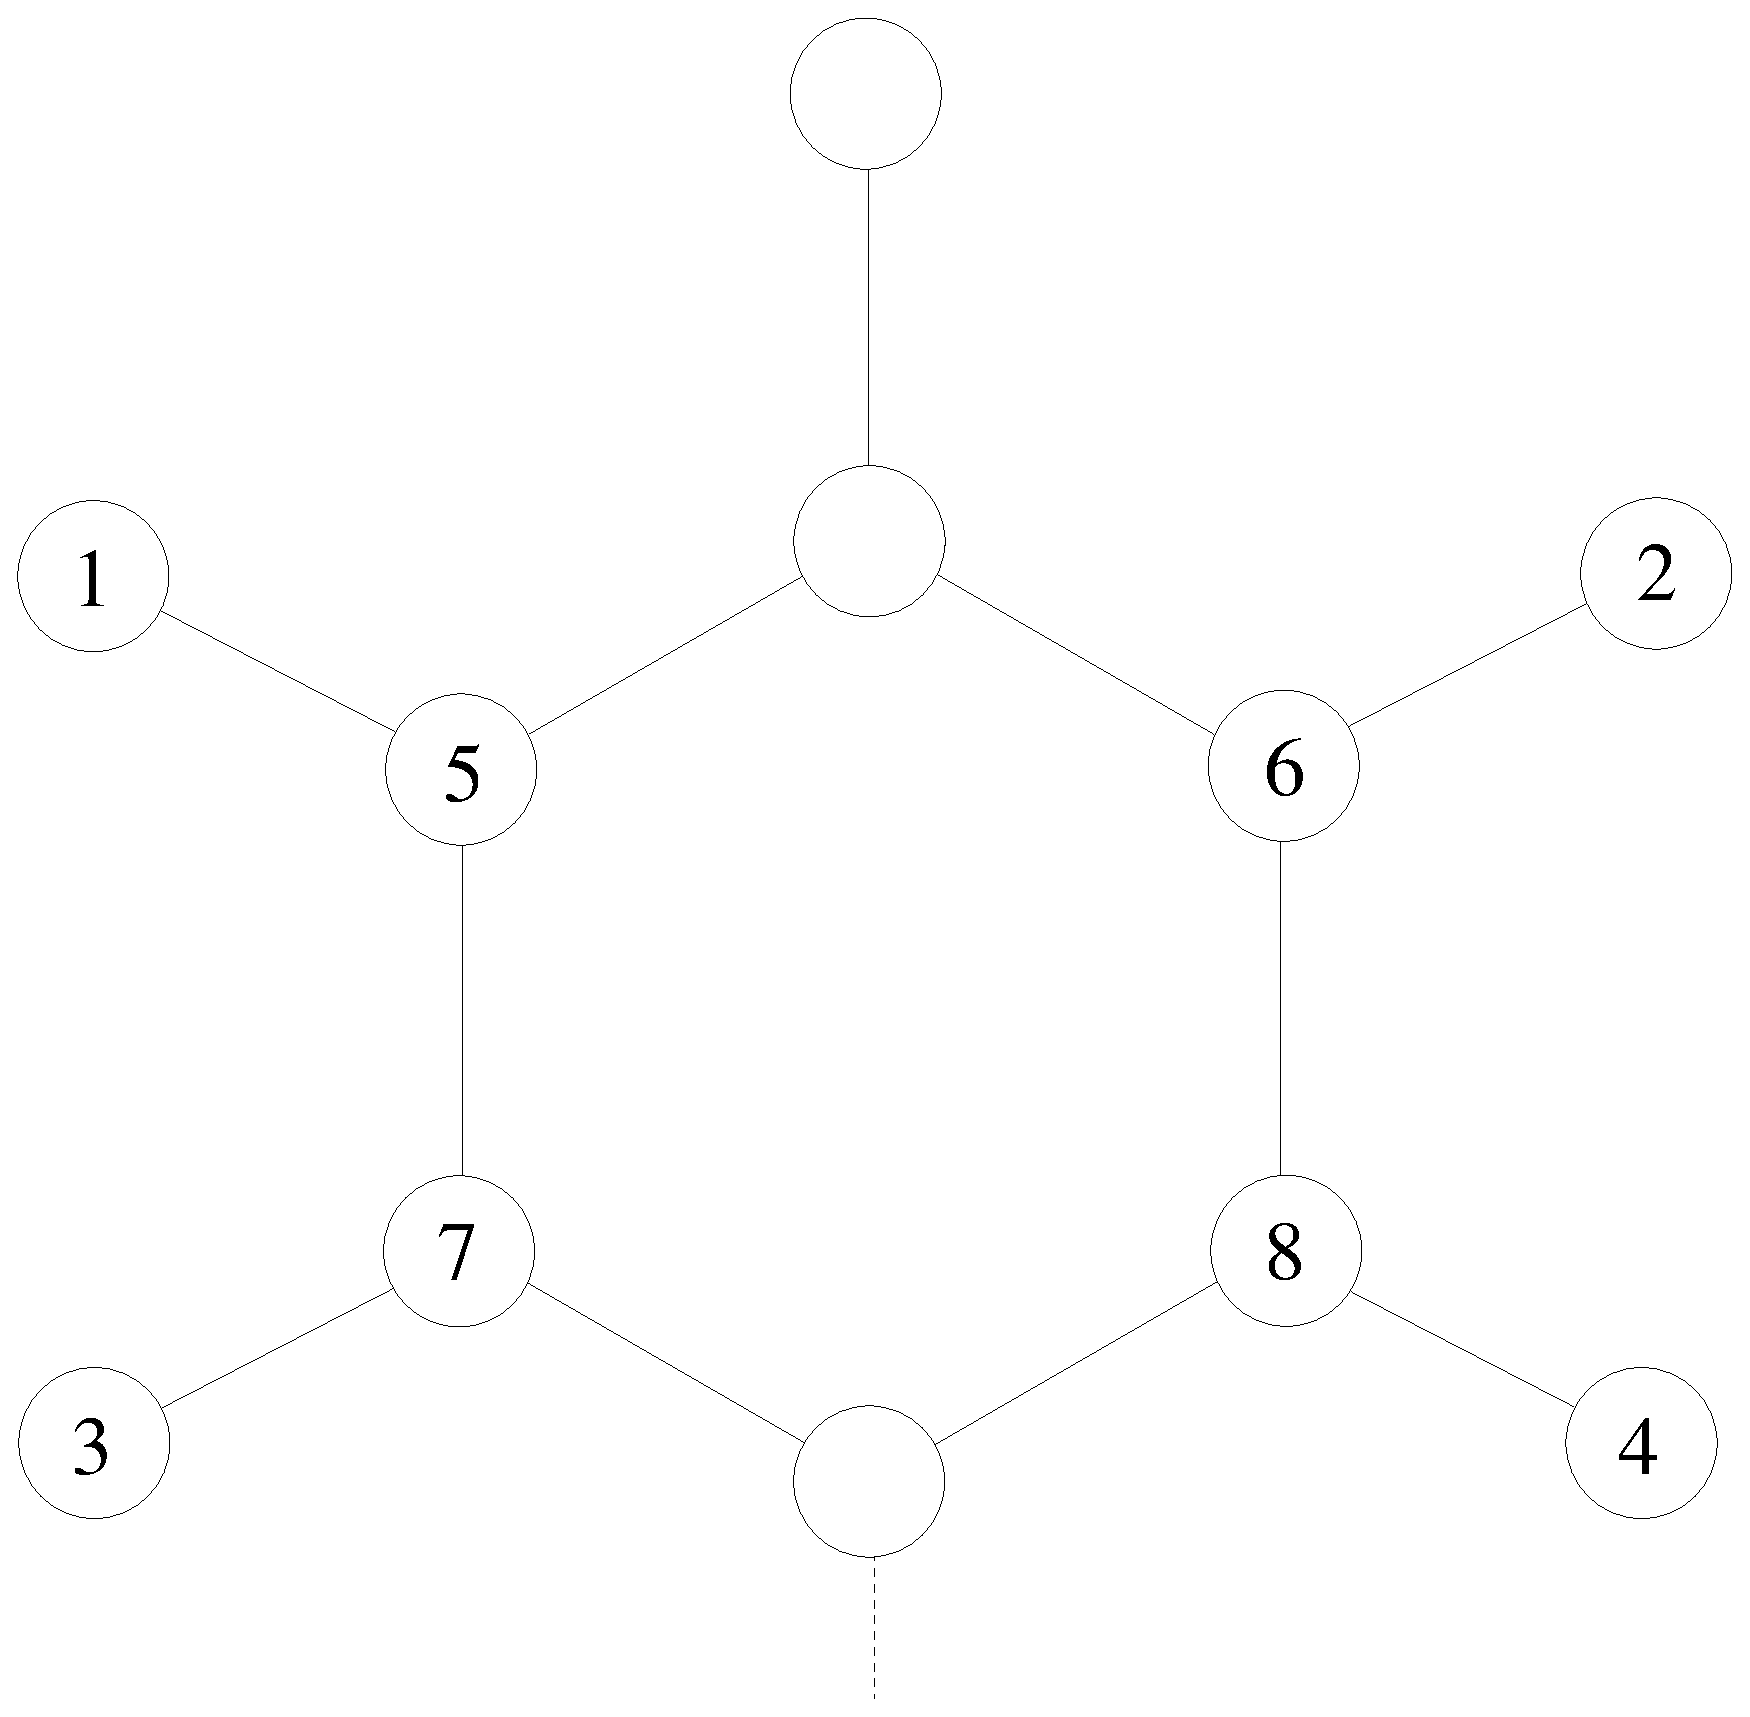
\includegraphics[width=0.5\textwidth]{PHE.eps}}
\end{figure}

For the phenylalanine example illustrated above we must allow three other pairs of
atoms to exchange if we swap 7 and 8. Hence a suitable {\tt perm.allow} entry is

{\textrm 1}

{\textrm 2 3}

{\textrm 7 8 5 6 1 2 3 4}

This should be on three consecutive lines.
Here $n=2$ and $s=3$: if we exchange 7 and 8 then we must also exchange 5 and 6,
1 and 2, and 3 and 4. There are two atoms in each of the three secondary sets, 
since we have specified 7 and 8 as the two primary atoms.

Here is an example {\tt perm.allow} file for a water trimer using
the flexible {\it QTIP4PF\/} potential, where the energy is invariant to permutations
of water molecules and to exchanges of hydrogens in the same molecule. However,
hydrogens cannot exchange between different oxygens:

{\textrm 4}

{\textrm 3 2}

% {\textrm 1 4 7 2 3 5 6 8 9}  sn402: I think this is wrong.
{\textrm 1 4 7 2 5 8 3 6 9}

{\textrm 2 0} 

{\textrm 2 3}

{\textrm 2 0} 

{\textrm 5 6}

{\textrm 2 0} 

{\textrm 8 9}

The first group of three oxygens has two atoms that must move with each oxygen,
i.e.~atoms 2 and 3 for oxygen 1, etc. Hydrogen permutations for each oxygen are
allowed by the three following groups. This scheme allows atoms to appear in more 
than one group. There must be a group containing each complete set of permutations
in order for permutation-inversion isomers to be recognised. The format
is compatible with an older scheme, where only pair swaps were allowed for
associated atoms, but now allows for more general permutations.

Scripts to generate allowed permutations automatically for CHARMM and AMBER are available from
the group web site. It is essential to use symmetrised versions of the corresponding
force fields! 

\item {\it PERMDISTINIT x\/}: performs the permutational analysis described above for {\it PERMDIST},
but only for the initial alignment of two end points. After this is done, the permutational
optimisation is turned off, which can save time.

\item {\it PERTDIHE chpmax chnmin chnmax iseed\/}: CHARMM 
and UNRES dihedral angle perturbation specification.
Performs random, {\tt GMIN}-style twists before starting optimisation.

\item {\it POINTS\/}: this is usually the last keyword and introduces the
coordinate information, which is read one atom per line. Each line must consist
of the atomic symbol of the atom followed by its three Cartesian coordinates.
Leading spaces before the atomic symbol should be avoided. For calculations
involving CHARMM, UNRES, AMBER and CPMD the coordinates are obtained from auxiliary files, 
and {\it POINTS\/} will be the last OPTIM directive in the {\tt odata} file, or
is not used (CHARMM and UNRES).

\item {\it PMPATH inr\/}: calculates the approximate steepest-descent pathways
leading from a transition state with the Page-McIver second order formulation.
{\it inr} can be 6 or 7, and has the same effect as the corresponding settings
for the {\it SEARCH\/} keyword. 
{\it inr\/}=6 should only converge to minima (default), while {\it inr\/}=7 
produces paths that can terminate at saddle points.

\item {\it PREROTATE\/}: For the GS and ES double-ended transition state
  search methods, if using {\it FIXATMS\/} to zero some coordinates of the
  forces to avoid overall translation and rotation, this keyword will rotate
  the start and end points so that those coordinates are zero in both.
The default is true.

\item {\it PRESSURE\/}: if present 
tells the program to perform a constant zero pressure optimisation
for bulk SC, ME, MP, MS and P6. Normally a constant volume optimisation takes place. 

\item {\it PRINT n\/}: sets the print level. The default value is zero. Use
of this option is not recommended, since more specific print control is possible.

\item {\it PRINTCOEFFICIENTS\/}: prints ground state coefficients for the MSEVB potential.

\item {\it PULL a1 a2 f\/}: apply a static force to the potential, equivalent to adding
the term $V_{\rm pull}=-f(z_{a1}-z_{a2})$. Here $z_{a1}$ and $z_{a2}$ are the $z$
coordinates for atoms $a1$ and $a2$, and $f$ specifies the force.
This potential is designed to simulate a pulling experiment with static force where
a molecule is pulled along the $z$ axis from atoms $a1$ and $a2$.

\item {\it PUSHCUT x\/}: sets the threshold for the RMS force below which the
system may apply a {\it PUSHOFF\/} to escape from a stationary point of the wrong Hessian
index. Default value is 0.00001. Using a negative value prevents pushoffs from
occurring.

\item {\it PUSHOFF x\/}: sets the magnitude of a step away from a stationary
point of the wrong Hessian index (see \S\ref{sec:scaling} for default action). Default value is 0.01.
Formally used as the step size in hybrid eigenvector-following
transition state searches if the eigenvalue of the direction being followed is positive.
{\it MAXMAX} has now replaced {\it PUSHOFF\/} in this role.

\item {\it PUSHOPT x conv max\/}: specifies that the magnitude of steps away from a transition state in 
path calculations should be calculated using a golden section search in the interval $[0:x]$ and
$[0:-x]$ for the tw directions. The search terminates when the pushoff magnitude for the
lowest energy in the line search is identified to an accuracy of {\it conv}, or when
{\it max} iterations have been performed.

\item {\it PV press gtol grad steps\/}: specifies an approximate constant pressure optimisation with
pressure {\it press\/} and convergence criterion {\it gtol\/} for the gradients with
respect to the box lengths. If any box length gradient is larger in magnitude than
{\it grad\/} then up to a maximum of {\it steps\/} optimisation steps for the box lengths
are performed.
If the three box lengths are equal to start with and the keyword {\it CUBIC \/} is included,
then a cubic box is maintained. 
Will not work with atom types MP, ME and MS.
Default values, {\it press\/}=0, {\it gtol\/}=0.001, {\it grad\/}$=10^{60}$, {\it steps\/}=100.

\item {\it PVTS press gtol grad nboxts\/}: as for {\it PV\/} but searches for a transition
state with respect to box length {\it nboxts\/}, where {\it nboxts\/}=1, 2 and 3 specify the
$x$, $y$ and $z$ box lengths, respectively. {\it nboxts\/} defaults to 1.

\item {\it PYG a1 a2 a3 b1 b2 b3 sigma0 eps0\/}: calls
a finite system of Paramonov-Yaliraki ellipsoids \cite{ParamonovY05}, where the potential involves
a set of eight parameters, six of them, $\{a_{k}\}$ and $\{b_{k}\}$ $(k = 1,2,3)$, defining two
different shape matrices for the repulsive and attractive parts of the interaction in terms of the
lengths of the semi-axes, and the other two, $\sigma_{0}$ and $\epsilon_{0}$, defining the length
and energy scales, respectively.

\item {\it QCHEM qchemjob sys\/}: calculate energy and gradient using the
{\tt QCHEM} program. {\it qchemjob\/} is a string specifying how to run
the {\tt QCHEM} executable, and {\it sys\/} is a string specifying the
{\tt QCHEM} input file.

\item {\it QTIP4PF\/}: flexible water potential from  Habershon {\it et al.}~[{\it J.~Chem.~Phys.\/}, 
{\bf 131}, 024501 (2009)] coded by Dr Javier Hern\'andez-Rojas.
The units of length and energy are \AA\ and kcal/mol. The atoms must be entered in the
order O, H, H, O, H, H, etc.

\item {\it QSPCFW\/}: flexible water potential from  Paesani {\it et al.}~[{\it J.~Chem.~Phys.\/},
{\bf 125}, 184507 (2006)] coded by Dr Javier Hern\'andez-Rojas.
The units of length and energy are \AA\ and kcal/mol. The atoms must be entered in the
order O, H, H, O, H, H, etc.

\item {\it RADIUS x\/}: specifies that atoms should not be allowed to move beyond a 
distance {\it x\/} from the origin.

\item {\it RANROT n\/}: for use with {\it PERMDIST\/}. Specifies
that {\it n\/} random orientations will be tried as well as the
initial standard alignment in {\tt minpermdist.f90}. Several hundred
random orientations may be needed to find the best translational/rotational/permutational
alignment of end points.

\item {\it RANSEED n\/}: specifies the initial seed for random number generation, as used in 
hard sphere moves with {\it FIXD}.

\item {\it RATIOS\/}: specifies that the pathway parameters needed to calculate catastrophe
ratios should be printed in a {\it PATH\/} run.

\item {\it RBSYM\/}: specifies that internal symmetry operations permuting equivalent sites for
rigid-body building blocks exist. The operations are read in from a file {\tt rbsymops}, which must
exist in the working directory. The first line of the file is an integer that specifies the number
of operations generated by proper axes of rotation including the identity operation; the operations
are then read in one at a time in a representation consisting of a unit vector, defining the
axis in the reference frame, and an angle in degrees, describing the magnitude of rotation about
that axis. The first operation has to correspond to the identity operation.

This keyword has to be combined with {\it PERMDIST\/} so that structures are aligned and
a distance metric considered based on permutations of identical rigid
bodies and any internal symmetry operation of each rigid body that is a symmetry
of the potential energy function.

\item {\it READMASS\/}: atomic masses will be read from file {\tt masses} in the
current working directory. This option may be useful for normal mode analysis
with potentials such as binary Gupta.

\item {\it READPATH\/}: if specified with {\it CALCRATES\/} then rate constants will be
calculated for the transition states found in {\tt path.info} and no stationary point
searches will be performed.

\item {\it READSP\/}: instructs {\tt OPTIM} to read minima and 
transition state data in the PATHSAMPLE format.
This has not been implemented yet!

\item {\it READHESS\/}: Hessian will be read from file {\tt derivs} at first step.

\item {\it READVEC\/}: if present the Hessian eigenvector
corresponding to the smallest eigenvalue 
will be read from file {\tt vector.dump}. The latter file can be generated using the
{\it DUMPVECTOR\/} keyword in a previous run.

\item {\it REDOPATH\/}: instructs {\tt OPTIM} to read transition state coordinates
successively from the file {\tt redopoints} during a {\it NEWCONNECT\/} run.
Can be used to generate movie files from stationary point sequences calculated
by PATHSAMPLE. The correct start and finish coordinates for the minima
must be present in the {\tt odata} and {\tt finish} files.

\item {\it REDOPATHXYZ\/}: as for {\it REDOPATH\/} above, except that existing
{\tt path.n.xyz\/} files are read instead of actually calculating pathways for the
transition states.

\item {\it REDOTS n\/}: The CONNECT algorithms often find the same refined TS multiple times. This keyword specifies that the first {\it n } times a TS is found, the pushoff path is calculated as normal. Subsequent times that the TS is found, the path is not calculated and the TS simply ignored. { \it n } has default value 2 (i.e. one re-try of the path run).

\item {\it REDUCEDBONDLENGTH blfactor CB\/}: rescales the bond lengths by a factor
of {\it blfactor} in the side chains of proteins, if modelled by one of the CHARMM
potentials. {\it blfactor} has to be specified, and its default value is one.
{\it CB} is an optional argument. When set, the bond length between the C$_{\alpha}$
and C$_{\beta}$ atoms is rescaled by {\it blfactor} as well, otherwise not.

\item {\it REOPT\/}: specifies that the eigenvector to be followed should be reoptimised
      in a BFGSTS search after the EF step and before the tangent space minimisation.
This is probably not a good idea. Default is false.

\item {\it REOPTIMISEENDPOINTS\/}: specifies that endpoint minima should be reoptimised
if their RMS force lies above the convergence threshold. Useful in connection 
runs where failure is guaranteed if one or more of the endpoints is not identified
as a minimum. A large RMS force at the beginning of a connection run driven
by PATHSAMPLE should be investigated because it suggests a problem, e.g.~with
{\it CHARMM\/} permutational isomerisations.
Default is false.

\item {\it REPELTS\/}: specifies that the transition state search direction should
be orthogonalised to the coordinates in file {\tt points.repel}.

\item {\it RESIZE x\/}: scales all the coordinates by {\it x}
before the first step is taken. 

\item {\it RIGIDINIT AACONVERGENCE \/}: This will turn on the local rigid body framework. This keyword needs two additional input files: {\it coordsinirigid\/} and {\it rbodyconfig\/}. {\it coordsinirigid\/} should contain the coordinates of all the atoms whether they are part of local rigid bodies or not. During initialization, OPTIM will select appropriate coordinates and throw away irrelevant ones. The format is: \\{\it x1 y1 z1} \\
{\it x2 y2 z2} \\
{\it ldots} \\
{\it ldots} \\
{\it xn yn zn} \\

The file {\it rbodyconfig\/} defines the rigid bodies, with the following format: \\
{\it GROUP NoAtomsInGroup} \\
{\it Atom 1} \\
{\it Atom 2} \\
{\it ldots} \\
{\it ldots} \\
{\it Atom N} \\

This keyword takes an optional argument {\it AACONVERGENCE \/}. If present, this switches on the use of the more accurate distance measure and method of calculating the RMS force for angle-axis coordinates described in this paper: V. Ruhle, H. Kusumaatmaja, D. Chakrabarti and D. J. Wales, {\it J. Chem. Theory Comput.}, 2013, {\bf 9}, 4026-4034.

\item {\it RIGIDMOLECULES\/}: For use only in conjunction with {\it RIGIDINIT}. Indicates a system composed of multiple rigid bodies and having no free atoms. This is a temporary keyword, used to isolate some parts of the rigid body code from the biomolecule potentials and similar. Most users probably don't need to use it, but talk to sn402 if you're unsure. Hopefully this keyword will soon be removed completely and its functionality absorbed into other keywords as appropriate.

\item {\it RING a1 a2...}: When using natural internal coordinates, specifies
  a ring that's not part of a PRO, PHE, TYR, TRP, or HIS residue. {\it a1,
  a2}, etc. are the atom numbers for the ring in consecutive order. Only rings
  of size 5 or 6 are permitted.

\item {\it RINGPOLYMER rpsyst nrp rpbeta }: Specifies a ring polymer system with harmonic springs between
  nrp images of the same system that generally have different geometries.
   rpsyst is a string specifying the system: AECK (asymmetric Eckart barrier), SD (Stillinger-David flexible water potential), TT (Xantheas' TTM3-F water), MCY 
   (VRT(MCY-5f) water), JB (James Bowman's water).\\
  nrp is the number of RP images.
  rpbeta is 1/kT in reduced units.
  {\it RINGPOLYMER} keyword takes the place of {\it POINTS} and must be the last
  keyword in the odata file before the points.
  
\item {\it RKMIN gmax eps\/}: calculates a steepest-descent path using gradient only
      information with convergence criterion {\it gmax\/} for the RMS force and initial
      precision {\it eps\/}. A fifth order Runga-Kutta algorithm is used.

\item {\it ROT\/}: if present a rotational kinetic energy term is
added to the Hamiltonian. Either constant angular momentum ({\it ROT JZ x\/}) or
constant angular velocity ({\it ROT OMEGA x\/}) may be used to specify $J_z$
or $\omega_z$.

% \item {\it SAVECANDIDATES\/}: % unknown

\item {\it SCALE n\/}: sets the scaling algorithm for eigenvector-following
steps, as described in \S\ref{sec:scaling}. The default is {\it n\/}=10.

\item {\it SCORE\_QUEUE\/}: specifies an Score parallel environment. 
Currently not used on group clusters.

\item {\it SEARCH n\/}: specifies the search type for eigenvector-following and
steepest-descent calculations based on second derivatives and Hessian diagonalisation, default is type 0.
The most common options are 0, a minimisation, and 2, a transition state search. See
\S\ref{sec:second} for full details.

\item {\it SHIFT x\/}: specifies the shift applied to eigenvectors corresponding
to normal modes that conserve the energy. The default is $10^6$. The shift {\it must\/} be
large enough to move the eigenvalues in question to the top of the spectrum.

\item {\it SLERP\/}: activates the iSLERP algorithm for rigid bodies when interpolating an initial band for the NEB. This algorithm (due to Li, X., J. Graphics Tools {\bf 12} (3), 1 (2011)) uses quaternions to provide an efficient route to smooth interpolation of a rigid body between two endpoints. Without this keyword, default behaviour is to interpolate rigid body coordinates as though they were cartesian. This is often not a problem, but can lead to uneven interpolation and occasionally very bad interpolated bands. The iSLERP algorithm seems to give reliably good interpolations.

\item {\it SQVV NIterSQVVGuessMax SQVVGuessRMSTol\/}:
specifies that the first {\it NIterSQVVGuessMax\/} DNEB refinements should be
done using the SQVV algorithm, rather than LBFGS.\cite{TrygubenkoW04}
The DNEB optimisation will switch to LBFGS minimisation after {\it NIterSQVVGuessMax\/}
steps or if the RMS force falls below {\it SQVVGuessRMSTol\/}.
The default values for {\it NIterSQVVGuessMax\/} and {\it SQVVGuessRMSTol\/}
are 300 and 2.0, respectively.

\item {\it ST muD E\/}: calls a finite system of Stockmayer particles,
where $\mu_{D}$ is the dipole moment strength and the electric field of stength $E$ can be optionally present. The field, if
present, is along the space-fixed z-direction.

\item {\it STEPMIN n\/}: sets the minimum number of optimisation steps before convergence
will be tested. The default is zero.

\item {\it STEPS n\/}: sets the maximum number of optimisation steps per call
to {\tt OPTIM}. The default is {\it n\/}=1. Setting {\it n\/} to zero at the start of a run
means that only a point group analysis is performed.

\item {\it STOCK $\mu$ $\lambda$}: sets the dipole moment strength and attraction prefactor
in the Stockmayer potential,
\begin{displaymath}
V_{ij} = 4\left(r_{ij}^{-12}-\lambda r_{ij}^{-6}\right) + \frac{\mu^2}{r_{ij}^3}
\left[\hat{\pmb\mu}_i\cdot\hat{\pmb\mu}_j-\frac{3}{r_{ij}^2}
(\hat{\pmb\mu}_i\cdot{\bf r}_{ij})(\hat{\pmb\mu}_j\cdot{\bf r}_{ij})\right].
\end{displaymath}
See also {\it STOCKSPIN}.

\item {\it STOCKSPIN x n}: Activates checking for alignment of dipoles with the $z$ axis in
the Stockmayer potential.  Such alignment makes the polar angle $\phi$ for the dipole
redundant, leading to extra zero Hessian eigenvalues and associated problems.  If alignment
is detected at any step in an optimisation then the orientation of the cluster is randomised
and a warning is printed.
$x$ is the amount by which $|\cos\theta|$ may differ from 1 for the dipole to be counted as
aligned with the $z$ axis.  $n$ is the maximum number of attempts to remove aligned dipoles
by random rotation.  Values of $10^{-4}$ and 10, respectively, are a sensible starting point.

\item {\it STOPDIST x\/}: in a {\it CONNECT\/} run, stop as soon as the distance between
the initial ({\it x}$>0$) or final ({\it x}$<0$) minimum and the furthest connected minimum
exceeds $|x|$.

\item {\it STOPFIRST\/}: in a {\it CONNECT\/} run, stop as soon as the initial minimum has a transition state
connection.

\item {\it SUMMARY n\/}: prints a summary of the steps and derivatives
every {\it n\/} steps. The default is $n=20$.

\item {\it SYMCUT x\/}: specifies the RMS force below which the point
group symmetry subroutine will be called. The default is {\it x\/}=0.001.

\item {\it TAG num massfac\/}:
allows atoms to be tagged. Atom number {\it num\/} has its mass increased
by a factor {\it massfac\/} for point group symmetry assignment only.
To tag more than one atom use additional {\it TAG\/} lines in {\tt odata}.

\item {\it TD\/}: add a tetrahedral field of strength {\it x} to the potential.

\item {\it TIMELIMIT x\/}: {\tt OPTIM} will stop if the accumulated cpu
time exceeds {\it x} seconds. The default value is infinity.

\item {\it TOLD x\/}: sets the initial distance tolerance for points
to be considered the same after rotations and reflections in point
group determination. The default is 0.0001.

\item {\it TOLE x\/}: sets the initial tolerance for eigenvalues
of the inertia tensor to be considered equivalent in point
group determination. The default is 0.0001.

\item {\it TOMEGA\/}: includes omega angles in the {\it TWISTDIHE\/} list.

\item {\it TOSI $A_{++}\ A_{--}\ A_{+-}\ \rho$\/}: specifies a Born-Mayer potential
with the parameters indicated (see \S\ref{sec:potentials}).

\item {\it TOSIC6 c6pp c6mm c6pm\/}: specifies additional C6 dispersion coefficients
for the {\it TOSI\/} potential. {\it c6pp, c6mm\/}, and  {\it c6pm\/} should be the values of the C6
parameters between positive ions, negative ions and positive and negative ions in atomic units
(see \S\ref{sec:potentials}).

\item {\it TOSIPOL alphap alpham damp\/}: specifies cation and anion polarisabilities in atomic units
and a damping parameter for the {\it TOSI\/} potential (see \S\ref{sec:potentials}).

\item {\it TRAD x\/}: sets the trust radius (see \S\ref{sec:scaling}). The default value is 2.0.

\item {\it TRAP k n\/}: general trapped ion potential coded by Ersin Yurtsever. 
The form of the potential is 
\begin{displaymath}
V=\frac{k}{2}\sum_i r_i^n + \sum_{i<j} \frac{1}{r_{ij}},
\end{displaymath}
where $r_i$ is the distance of ion $i$ from the origin and
$r_{ij}$ is the distance between ions $i$ and $j$.

\item {\it TSIDECHAIN\/}: includes sidechain angles in the {\it TWISTDIHE\/} list.

\item {\it TSPLITTING\/}: Tunnelling splittings of the vibrational ground state level following
\cite{ric11}. Every time a rate is calculated, the tunnelling splitting
is calculated as well. Tunnelling splittings only make sense for
symmetric molecules and barriers.


\item {\it TTM3\/}: specifies Xantheas' TTM3-F water potential, coded
by Jeremy Richardson.
The atom order must be O1, O2,\ldots, H1a, H1b, H2a, H2b,\ldots.
The energy is in kcal/mol and the distance unit is \AA.
Hydrogens are NOT permutable between different oxygens.

\item {\it TWIST n1 n2 n3 n4 f ref\/}: adds a twist potential corresponding to the
torsional angle for atoms {\it n1}, {\it n2}, {\it n3} and {\it n4}.
The functional form is $V_{\rm twist}(\phi)=f\sin(\phi-\phi_{\rm ref}$.
$phi_{\rm ref}$ and the angular displacement are set to the range $-\pi$ to $\pi$,
but with the sin function dependence this should now make no difference.
% Geometry optimisations will start to fail if the angular displacement reaches either
% end of this range, which limits the value of $f$.
Setting $\phi_{\rm ref}$ to the angle for the global minimum or native state might
be convenient.

\item {\it TWISTDIHE random xpert\/}: twist phi/psi dihedral angle selected from an array of safely
twistable dihedrals using the random number {\it random\/} between 0 and 1 by {\it xpert\/} degrees before 
starting optimisation. This keyword is no longer designed to be user specified, but is used by PATHSAMPLE.

\item {\it TWISTTYPE n\/}: integer {\it n\/} specifies the type of dihedral angle twisting
used to  guess transition states in {\bf guessts} for CHARMM and UNRES.
The recommended value is {\it n}=5. See also {\it NORANDOM\/}.

\item {\it TWOENDS fstart finc ntwo rmstwo ntwoiter twoeval\/}: obsolete: specifies a double-ended transition
state search. {\it fstart\/} is the initial force constant pulling the coordinates towards the final
geometry which is read from a file named {\tt final}. {\it finc\/} is the increment for the force 
constant after each cycle. {\it ntwo\/} is the maximum number of minimisation steps taken after each
increment of the force constant, and {\it rmstwo\/} is the convergence condition on the RMS force
for these minimisations. {\it ntwoiter\/} is the total number of force constant increments allowed
and {\it twoeval\/} is the value of the smallest Hessian eigenvalue below which the program will
shift to a transition state search.

\item {\it UACHIRAL\/}: MUST be included when using ff03ua, the AMBER united atom forcefield. It ensures the correct impropers are used to define sidechain 
chirality when HB hydrogen is missing.

\item {\it UNRES\/}: specifies the UNRES potential, which requires an UNOPTIM executable.
An auxiliary file {\tt coords} is required. {\it UNRES} must be the last OPTIM directive in the
{\tt odata} file. The remaining content of {\tt odata} consists of UNRES keywords and
setup information.

\item {\it UPDATES mupdate1 mupdate2 mupdate3 mupdate4\/}: 
specifies the number of updates in the LBFGS routine before
      resetting. 
{\it mupdate1\/} is used for energy minimisation, 
{\it mupdate2\/} is currently ignored by {\bf mind},
{\it mupdate3\/} is used in Rayleigh-Ritz eigenvalue calculations, and 
{\it mupdate4\/} is used in NEB and DNEB optimisation. 
{\it mupdate5\/} is used in string method optimisation. 
The default value is 4 for all five parameters.

\item {\it USEDIAG n\/}: allows different approximations to be used for the 
eigenvalue in a Rayleigh-Ritz {\it BFGSTS\/} calculation. $n=1$ specifies the
second order central differences method.
$n=2$ is the same accuracy, but uses a formula that minimises the rounding
error, which may work better for numerically large values of the energy and
is the default behaviour. $n=3$ specifies the first order forward finite 
differences method which is less accurate, but requires one fewer potential 
call per iteration.

\item {\it USEEV n \/}: specifies the number of non-zero (lowest) eigenvalues and
eigenvectors to be calculated by LAPACK routine DSYEVR in {\bf efol.f},
{\bf bfgsts.f} or {\bf hybridmin.f}.
If this value is not specified than full diagonalisation is performed in 
{\bf efol.f} using LAPACK routine DSYEV, while the default is a single
eigenvalue/eigenvector for {\bf bfgsts.f} and {\bf hybridmin.f}.

\item {\it VALUES n\/}: prints the Hessian eigenvalues every {\it n\/} steps.
The default is {\it n\/}=20.

\item {\it VARIABLES\/}: optimises a general function (which must be specified in
{\bf potential}. The initial values of the variables are read one per line after the {\it POINTS\/}
keyword in {\tt odata}.

\item {\it VARSTEPOPT\/}: Allows instanton optimization with a variable step size distributino of the beads as described in \cite{Rommel2011b}.

\item {\it VASP vaspjob\/}: tells {\tt OPTIM} to use the {\tt VASP} 
executable to calculate energies and gradients.
The string {\it vaspjob\/} specifies the run command for {\tt VASP}.

\item {\it VECTORS n\/}: prints the Hessian eigenvectors every {\it n\/}
steps. Eigenvector printing is turned off by default.

\item {\it WARRANTY\/}: print warranty information.

\item {\it WELCH $A_{++}\ A_{--}\ A_{+-}\ \rho\ Q_+\ Q_-\ \alpha_+\ \alpha_-$\/}: specifies a Welch binary
salt potential with the parameters indicated (see \S\ref{sec:potentials}).

\item {\it ZEROS n\/}: sets the number of zero Hessian eigenvalues to be
assumed---useful for general optimisation problems specified by {\it VARIABLES\/}. 
\end{itemize}
% </kwd>

\section{Specification of Potentials}
\label{sec:potentials}
There follows a list of some of the 
potentials that the program understands. These are introduced according to the atom
type by which they are identified.

\subsection{AR}Lennard-Jones potential with $\sigma$ appropriate for Ar,
i.e.~$3.4\,$\AA. Hence, input is expected in Angstrom and energies are calculated
for $\epsilon=1$. Subroutines used: {\bf ljdiff}.

\subsection{AU, AG and NI}These types specify Sutton-Chen potentials of the appropriate
form.\cite{suttonc90}\ 
Three additional real parameters must be specified using the {\it PARAMS\/} keyword
in the {\tt odata} file,
namely Sutton and Chen's $\epsilon$, $c$ and $a$, in this order.
The nearest neighbour distance in the prevailing unit system is $a/\sqrt{2}$. Hence,
using $a=\sqrt{2}$ corresponds to a unit system where the bulk nearest-neighbour distance is 1.
Subroutines used: {\bf scdiff}.

\subsection{AX}Lennard-Jones potential plus a variable quantity of the Axilrod-Teller
triple-dipole term\cite{wales90c,doyew92}\ with units $\sigma=\epsilon=1$. 
The pre-multiplication factor for
the three-body term, $Z^*$, is specified by the {\it PARAMS\/} keyword.
If a multiplier of $0.0$ is specified the Axilrod-Teller derivatives
and energy are not calculated, thus providing a route to the pure Lennard-Jones potential
in reduced units. Subroutines used: {\bf ardiff}, {\bf apairs}, {\bf axdiff}, {\bf axpairs}.

\subsection{AZ}Aziz argon potential from {\it J.~Chem.~Phys.\/}, {\bf 99}, 4518, 1993.
Input coordinates are assumed to be in units of $\sigma$ and the energy is given in
units of $\epsilon$.

\subsection{BC}Binary Lennard-Jones system, as for atom type LS, but without periodic
boundary conditions. Subroutine used: {\bf ljpshiftbinc}.

\subsection{BE}This specifies a trapped ion potential.\cite{walesl93}\
Subroutines used: {\bf etrap}, {\bf dtrap}.

\subsection{C1}A ten-bead model produced by cutting down the usual P46 potential specified
by atom type PL. Subroutine used: {\bf c10}.

\subsection{C6}This type specifies Girifalco's C$_{60}$ intermolecular potential.\cite{girifalco92}\
The energy is returned in units of the pair well depth; distances are in units of $3.4690\,$\AA.
Subroutines used: {\bf c60diff}.

\subsection{CADPAC}If keyword {\it CADPAC\/} is set in {\tt odata} then
OPTIM will try to read the derivatives from file {\tt derivs} in the
standard CADPAC\cite{CADPAC}\ punch format. 
It will also try to read the energy for the geometry
corresponding to these derivatives from a file called {\tt cadenergy}, which is optional.

\subsection{CC}This uses the two- plus three-body potential of Balm \etal\ for carbon.\cite{balmakm91} 
Subroutines used: {\bf jmecc}, {\bf jm2cc}, {\bf jm3cc}.

\subsection{CD}Specifies a potential for rigid-body pentagonal pyramids. In this case the
rigid body coordinates are three centre-of-mass parameters and three components of a 
vector that specifies a rotation axis and magnitude. The orientational coordinates are stored
after all the centre-of-mass coordinates. Subroutine used: {\bf capsid}.

% \subsection{CL}This is used to specify a Born-Meyer potential for $\rm (KCl)_n$ clusters
% using the same parameters as Rose and Berry.\cite1\ 
% \endnote{J.~P.~Rose and R.~S.~Berry}{\jcp}{96}{517}{1992}
% The atoms must be in the order K, Cl,
% K etc. Atomic units are assumed. Subroutines used: {\bf kdiff}, {\bf kpairs}.

\subsection{CK}Specifies a two-dimensional trapped-ion cluster. Subroutines used:
{\bf ectrap} and {\bf dctrap}.

\subsection{DZ}Dzugutov potential:\cite{Dzugutov92,Dzugutov93b}
\begin{eqnarray}
V(r)&=&A(r^{-m}-B) \exp\left( {c\over r-a}\right) \Theta(a-r) + 
    B \exp\left({d\over r-b}\right) \Theta(b-r). \nonumber
\end{eqnarray}
Seven parameters must by specified by a {\it PARAMS\/} line in the {\tt odata} file,
i.e.~$m$, $A$, $c$, $a$, $B$, $d$, and $b$.

\subsection{FH}Will read derivatives from file {\tt fhderivs} generated by the Fenske-Hall approximate
SCF package.\cite{hallf72}

\subsection{GAUSSIAN}If keyword {\it GAUSSIAN\/} is set in {\tt odata} then
OPTIM will try to read the derivatives from file {\tt derivs} in the
standard GAUSSIAN punch format.
It will also try to read the energy for the geometry
corresponding to these derivatives from a file called {\tt cadenergy}, which is optional.

\subsection{GL}This type specifies a G\={o}-type model\cite{uedatg78} for the
46-bead three-colour model polypeptide specified by atom type Pl below. 
All the attractive $1/R^6$ terms are turned off except for those between
native contacts in the global minimum, which are unchanged.
Subroutines used: {\bf g46merdiff}.

\subsection{GO}Paul Whitford's G\={o} BLN-type potential.

\subsection{IN}This is used to specify a shielded Born-Meyer potential binary ionic clusters with
anions and cations having the same magnitude charge.
The atoms must be in the order cation, anion, cation, anion, etc. The energy is:
$$ E = \sum_{i<j} \left[ {q_iq_j\over r_{ij}} e^{-\gamma r_{ij}} + A_{ij}e^{-r_{ij}/\rho_{ij}} \right]. $$
The parameters that can
be specified with {\it PARAMS\/} are $\gamma$, the magnitude of the ionic charges, a single
value of $\rho$, assumed to be the same for all interactions, and $A_{++}$, $A_{--}$ and
$A_{+-}$, in order. Default values for KCl are set for all parameters except $\gamma$.
Atomic units are assumed. Subroutines used: {\bf ions}.

\subsection{JC}This uses Murrell's two- plus three-body 
potential.\cite{murrellm90,murrellr90,alderzijmr91,eggenjlm92,fengjm93} 
A file {\tt JMparams} must
exist in the current directory containing the parameters $c_0,\ c_1,\ldots,\ c_{10},\ r_e,\ 
D,\ a_2$ and $a_3$. Subroutines used: {\bf jmec}, {\bf jm2c}, {\bf jm3c}.

\subsection{JM}This uses Murrell's two- plus three-body 
potential\cite{murrellm90,murrellr90,alderzijmr91,eggenjlm92,fengjm93} with periodic boundary
conditions (minimum image convention.\cite{allent87} 
A {\tt JMparams} file must exist as for type JC. (In previous versions the 
first three lines of {\tt JMparams} were assumed to contain
the square roots of 2, 3 and 6). Four additional real parameters must be given after the
search type and maximum step size specification, these being the $x$, $y$ and $z$ dimensions
of the periodic cell and the cutoff, respectively. I do not think the code has been tested
for any non-cubic unit cells. The cutoff should not be greater than half the box length.\cite{allent87}
Subroutines used: {\bf jmep}, {\bf jm2p}, {\bf jm3p}.

\subsection{LM}Specifies a Mason-Schamp potential\cite{Mason58} for a rare gas--alkali metal ion cluster
such as Ar$_{N}$Li$^+$. The three parameters $\epsilon$, $R_m$ and $\gamma$
must be set using the {\it PARAMS\/} keyword in {\tt odata}.

\subsection{LP}This type specifies the Lennard-Jones potential with 
periodic boundary conditions (minimum image convention.\cite{allent87}
The box lengths in the $x$, $y$ and $z$ 
directions and the cutoff (as a fraction of the smallest box length)
must be specified using the {\it PARAMS\/} keyword in the {\tt odata} file.
Setting a negative value for the cutoff fraction means that all minimum
images are included.
Subroutines used: {\bf ljpdiff}.
If the {\it BINARY\/} keyword is specified then a binary Lennard-Jones
potential is used\cite{sastryds98} along with subroutine {\bf ljpbin} or {\bf ljpshift}.

\subsection{LS}This type specifies shifted, truncated Lennard-Jones potential with 
periodic boundary conditions as for LP above. The {\it BINARY\/} keyword must also be 
specified.

\subsection{LC}This type specifies shifted, truncated Lennard-Jones potential with 
periodic boundary conditions, as for LS above, except that the neighbour list is not
updated when FIXIMAGE is set. The {\it BINARY\/} keyword must also be 
specified. See also {\it FIXAFTER}.

\subsection{LM}Lennard-Jones potential with a mean-field long range correction.

\subsection{M}This specifies a Morse potential with $D=r_e=1$. 
The remaining range parameter,\cite{braierbw90} $\rho_0$, must be specified using the {\it PARAMS\/} keyword
in the {\tt odata} file.
Subroutines used: {\bf mpairs}, {\bf mdiff}.

\subsection{ME}Specifies the generic Mie potential with periodic boundary conditions (minimum
image convention). Six extra parameters must be specified in the {\tt odata} file using the
{\it PARAMS\/} keyword;
in order these are the exponents {\it n\/} (repulsive) and $m$ (attractive), the three box
lengths and the cutoff. If keyword {\it PRESSURE\/} is set in {\tt odata}
then a constant pressure type optimisation is performed
using golden section minimisation, as described for SC. Note that
{\it n\/} and {\it m\/} should both be entered as reals. Subroutines used: {\bf emie}, {\bf mied}
and {\bf miel}. 

\subsection{MP}This type specifies the Morse potential with 
periodic boundary conditions (minimum image convention\cite{allent87}). 
The range parameter, $\rho_0$, the box lengths in the $x$, $y$ and $z$ 
directions and the cutoff (as a fraction of the smallest box length)
must be specified using the {\it PARAMS\/} keyword in the {\tt odata} file.
If the keyword {\it PRESSURE\/} is set in the {\tt odata} file
then a constant pressure optimisation is performed
with the energy being minimised by eigenvector-following with respect to the 
box lengths at every step. 
The cutoff is automatically changed in proportion to the change in box size.
Otherwise the optimisations are performed at constant volume, with no 
relaxation of the unit cell. 
Subroutines used: {\bf mpdiff}, {\bf mlatmin}.

\subsection{MS}This type specifies the Morse potential with 2-dimensional
periodic boundary conditions.
The free surfaces are perpendicular to the $z$ direction at the top and bottom
of the cell.
The range parameter, $\rho_0$, the box lengths in the $x$ and $y$ 
directions and the cutoff (as a fraction of the smallest box length)
must be specified using the {\it PARAMS\/} keyword in the {\tt odata} file.
If the keyword {\it PRESSURE\/} is set in the {\tt odata} file
then a constant pressure optimisation is performed
with the energy being minimised by eigenvector-following with respect to the 
box lengths at every step. 
The cutoff is automatically changed in proportion to the change in box size.
Otherwise the optimisations are performed at constant volume, with no 
relaxation of the unit cell. 
Subroutines used: {\bf msdiff}, {\bf mslatmin}.

\subsection{NIMET}
The keyword NIMET specifies a density based embedded atom
method (EAM4) for the chemisorption of hydrogen on a Ni(100) surface\cite{Foiles86,Daw84,Truong90a,Truong90b}.
The structural model that can be used so far for the diffusion of H
on Ni(100) consists of a single hydrogen atom adsorbed on a
four-layered slab of 392 Ni atoms, with 98 atoms in each layer.
This number of Ni atoms was chosen so that the length of the
simulation box in the two lateral directions was more than twice
the cutoff distance of the EAM4 potential (10 \AA{}).\cite{Truong90b} Periodic
boundary conditions are employed in the two dimensions
parallel to the surface, and the bottom layer of the lattice is
held fixed. 


\subsection{NIHEAM7}
The keyword NIHEAM7 specifies an embedded atom
method (EAM7) for the chemisorption of hydrogen on a Ni(100) or Ni(111) or Ni(110)
surface\cite{Foiles86,Daw84}.
The structural model is as in NIMET (EAM4). The functional forms combine 
EAM4,\cite{Truong90a,Truong90b} EAM5,\cite{Wonchoba95} EAM6,\cite{Wonchoba96} and EAM7\cite{Wonchoba98}.
Be aware that the parameters were to crudly approximated and some functions had typos in the 
original EAM6 paper so they have been taken from the original f77 code and this paper\cite{Kindt99} .
The gradient correction for the hydrogen embedding function in EAM6 is neglected at the moment, 
since the original code doesn't include it as well.


\subsection{P6}This type specifies Girifalco's C$_{60}$ intermolecular potential\cite{girifalco92}
with periodic boundary conditions (minimum image convention\cite{allent87}). If keyword
{\it PRESSURE\/} is specified in {\tt odata}
then a constant pressure type optimisation is performed,
as described for SC, above. However, in this case the lattice constant optimisation is
achieved by eigenvector-following. As for SC, the cutoff is changed in proportion to
the box size. Four extra parameters must be specified in the {\tt odata} file using the
{\it PARAMS\/} keyword,
as for SC. Subroutines used: {\bf latmin}, {\bf c60p}.

\subsection{PL}This type specifies a 46-bead three-colour model polypeptide. 
See also the corresponding G\={o} model potential.
Subroutines used: {\bf p46merdiff}.

\subsection{PR}This type specifies the Pacheco-Ramelho C$_{60}$ intermolecular potential\cite{pachecor97}
The value of the Axilrod-Teller parameter should be specified as the first argument to the
PARAMS keyword.

\subsection{SC}This type specifies the Sutton-Chen potential\cite{suttonc90} with periodic boundary
conditions (minimum image convention\cite{allent87}). 
If no file named {\tt SCparams} exists in the current 
directory the 12\mydash6 potential for gold is used. Otherwise the Sutton-Chen
parameters $n,\ m,\ \epsilon,\ c$ and $a$ are read from this file in order. If the
keyword {\it PRESSURE\/} is set in the {\tt odata} file
then a constant pressure optimisation is performed
with the energy being minimised by golden section with respect to the cubic box size before taking another
step. The cutoff is automatically changed in proportion to the change in box size.
Otherwise the optimisations are performed at constant volume, with no relaxation of the
unit cell. The bulk fcc nearest neighbour distance in the prevailing unit system is $a/\sqrt{2}$,
as above.
Subroutines used: {\bf escp}, {\bf dscp}.

\subsection{SI}This uses Murrell's two- plus three-body potential for Si\cite{lijm92}.
Subroutines used: {\bf jme}, {\bf jm2}, {\bf jm3}.

\subsection{SM} Specifies the Stillinger-Weber two- plus three-body potential for Si\cite{stillingerw85}
with the three-body part increased by 50\%.
Subroutines used: {\bf SWtwo}, {\bf SWthree}, {\bf SWlatmin}.

\subsection{SW} Specifies the Stillinger-Weber two- plus three-body potential for Si\cite{stillingerw85}.
Subroutines used: {\bf SWtwo}, {\bf SWthree}, {\bf SWlatmin}.

\subsection{Tosi}This keyword specifies a Born-Mayer potential of the form
$$ E = \sum_{i<j}\left[ {q_i q_j\over r_{ij}} + A_{ij}\exp(-r_{ij}/\rho) \right]. $$
The sum runs over all ions. Tosi-Fumi\cite{tosif64} parameters in atomic units should be
entered after the Tosi keyword in the order $A_{++}$, $A_{--}$, $A_{+-}$, $\rho$.
The ions are then specified using atom types PL and MI for plus and minus, respectively,
and can be in any order. There need not be equal numbers of positive and negative ions.
C6 dispersion coefficients can be optionally added with the keyword {\it TOSIC6 c6pp c6mm c6pm\/},
where {\it c6pp, c6mm\/}, and  {\it c6pm\/} should be the values of the C6 parameters between positive ions,
negative ions and positive and negative ions in atomic units. First order induction energy
can be added with the keyword {\it TOSIPOL alphap alpham damp\/} where {\it ALPHAP\/} and
{\it ALPHAM \/} are the cation and anion polarisabilities in atomic units and {\it DAMP\/}
is the damping parameter, without which cold fusion is likely. Note that the Welch potential
has been fitted to include ion polarisabilities and is described below.

% \subsection{TB}Tersoff-Brenner potential for carbon\cite1---numerical second derivatives only.
% \endnote{D.~W.~Brenner}{J.~Phys.~Rev.~B}{42}{9458}{1990}
% Subroutines used: {\bf tbe}, {\bf tbdiff}.

\subsection{TH} Specifies the Thomson problem. Two times the number of ions
must be divisible by three.

\subsection{TT} Specifies a tight-binding potential. 
Subroutines used: {\bf tighte}, {\bf secsi}.

\subsection{Welch}This keyword specifies a Welch potential\cite{welchld76,phillipscb91} of the form
\begin{eqnarray*}
E &= \sum_{i<j}\Bigg[ {\D q_i q_j\over\D  r_{ij}} + A_{ij}\exp(-r_{ij}^{\rm eff}/\rho) 
              -{\D q_i({\bf \mu}_j\cdot{\bf r}_{ij})\over\D  r_{ij}^3} 
              -{\D q_j({\bf \mu}_i\cdot{\bf r}_{ji})\over\D  r_{ij}^3} \\
             &-3{\D   ({\bf \mu}_i\cdot{\bf r}_{ij})
                   ({\bf \mu}_j\cdot{\bf r}_{ij})\over\D  r_{ij}^5} 
              +{\D  {\bf \mu}_i\cdot{\bf \mu}_j\over\D  r_{ij}^3}\Bigg] 
              +\sum_i {\D \mu_i^2\over\D 2\alpha_i}, \\
\end{eqnarray*}
where 
$$ {\bf r}_{ij}^{\rm eff}={\bf r}_{ij}+{{\bf\mu}_i\over Q_i}-{{\bf \mu}_j\over Q_j}, 
    \qquad r_{ij}^{\rm eff}=\left|{\bf r}_{ij}^{\rm eff}\right|. $$
Welch parameters in atomic units should be
entered after the Welch keyword in the order $A_{++}$, $A_{--}$, $A_{+-}$, $\rho$, $Q_+$,
$Q_-$, $\alpha_+$, $\alpha_-$.
The ions are then specified using atom types PL and MI for plus and minus, respectively,
and can be in any order. There need not be equal numbers of positive and negative ions.

\subsection{W1, W2, W3, W4}Specifies that each {\tt odata} entry gives the centre of mass coordinates
of a rigid water molecule to be described by a TIPS potential\cite{jorgensen81} of type 1, 2, 3 or 4.
The Euler angles then follow all the centre of mass coordinates, again three per line.
Subroutines used: {\bf h2o}.

\subsection{Z1, Z2}These are the two forms of the Zetterling potential:\cite{DoyeWZD03}
\begin{equation}
V(r)=a {e^{\alpha r}\over r^3} \cos(2k_F r)+b\left({\sigma\over r}\right)^{n}+V_0.
\end{equation}
Subroutines used: {\bf Z1} and {\bf Z2} etc.
If three parameters are specified by the {\it PARAMS\/} keyword they are interpreted 
as box lengths for a periodic system.

% \subsection{A1, A2, A3, A4}Used for a benzene-Ar$_n$ cluster with four slightly different
% potentials. In each case the benzene molecule has a fixed geometry which is not read in.
% Potentials for A1 and A3 include the induction energy, while A2 and A4 do not. Potentials
% A1 and A2 use one set of Lennard-Jones parameters while A3 and A4 use a different set\cite1.
% \endnote{D.~J.~Wales}{\molphys}{74}{1}{1991}
% Subroutines used: {\bf bzgeom}, {\bf bzarlj}, {\bf ljdiff}, {\bf bzarin}, {\bf indiff}.

\subsection{Rotating Clusters}If keyword {\it ROT\/} is set in 
{\tt odata} then additional terms will be added to the
energy and the derivatives corresponding to the kinetic energy for rigid body rotation
about the space fixed $z$ axis. Either the angular momentum or the angular velocity
may be fixed using {\it ROT J2Z\/} or {\it ROT OMEGA2\/} followed by the value.

\section{Second-Derivative Based Searches}
\label{sec:second}
At present there are eight possible single-ended search types 
that employ Hessian calculation (or update) and full diagonalisation. They are specified by
the {\it SEARCH\/} keyword with a parameter 
represented by the internal integer variable INR, with allowed values ranging from 0 to 7. 
The two most common
types are 0, for minimisation, and 2, for transition state searching. The steps have
the same form in both cases,\cite{wales94a} except that we go downhill in every direction when
minimising, and uphill in one direction when looking for a transition state. For these
search types convergence to stationary points with the wrong Hessian index (i.e.~not
0 or 1 negative Hessian eigenvalues, respectively) is detected and countermeasures are
taken as specified below. 

The eigenvector to be followed `uphill'
in an eigenvector-following transition state search is specified by an integer following the keyword 
{\it MODE\/} in {\tt odata}.  We count up from the eigenvector corresponding to 
the smallest eigenvalue, the one corresponding to the second smallest eigenvalue 
etc.~using values 1, 2 and so on. The value specified by {\it MODE\/} is only
effective on the first step: for subsequent steps the critical eigenvector is 
chosen by a maximum overlap criterion using the dot product with the eigenvector 
that was followed at the previous step.  Using {\it MODE\/} 0 means that the 
eigenvector corresponding to the smallest Hessian eigenvalue is chosen at every step. 

Quite often, especially if we are taking large steps in a region far from convergence,
the largest modulus dot product may fall well below unity and give rise to ambiguity.
At present the program takes the following action if the maximum overlap is less than
0.7. The chosen eigenvector is simply set to the same one that was followed in the last
step, where the eigenvectors are numbered in terms of the corresponding eigenvalues arranged in
ascending order. Zero eigenvalues are excluded from the counting. The same action is
taken if the maximum overlap is with an eigenvector lying more than 8 places above
the one followed at the previous step, when arranged according to ascending eigenvalue.

The behaviour for other search types is as follows. {\it SEARCH\/} 1
specifies a pseudo-Newton-Raphson search where the formula for the steps is the same
as the eigenvector-following step for search types 0 and 2, but we search uphill or
downhill depending only upon the sign of the eigenvalue corresponding to the direction
in question.\cite{wales94a}
Of course, this step tends to the conventional Newton-Raphson step
near a stationary point. For {\it SEARCH\/} 1 convergence to stationary points of any Hessian 
index is allowed.

Search types 3 and 4 are the same as 0 and 2 except that a pseudo-third derivative
correction is applied to the step\cite{wales94a}. These search types are now {\bf redundant}
because dynamic scaling using a trust radius and separate maximum step sizes for each
direction seems to work much better (see \S\ref{sec:scaling}).

Search type 5 is the same as type 0 except that the system is rotated into principal
axes first.

Search types 6 and 7 are for steepest-descent energy minimisations using the Page-McIver
method\cite{pagem88} with analytic first and second derivatives at each step. 
Search type 7 can converge to a saddle point, search type 6 can only converge to a true minimum.

Search type 8 is a steepest-ascent transition state search using a modification of
the Page-McIver steepest-descent algorithm.

Search types 0, 6 and 7 can be used as minimisers for pathway calculations.
In this case it is possible to use a subset of eigenvalues and eigenvectors
by supplying {\it USEEV n \/} in {\tt odata}.
The number of second derivative-based minimisation steps can be controlled
with {\it PATHSDSTEPS n\/}, after which {\tt OPTIM} will switch to LBFGS.

\section{Gradient-Only and Hybrid Searches}
\label{sec:gradient}
It is generally much more efficient to carry out energy minimisation, including
pathway calculations, using the LBFGS gradient-only routine specified by
{\it BFGSMIN\/}. Steepest-descent
paths or minimisations can also be calculated by Runge-Kutta or Bulirsch-Stoer integration
using the {\it RKMIN\/} and {\it BSMIN\/} keywords, respectively.

A hybrid BFGS/eigenvector-following
transition state search\cite{munrow99,kumedamw01} can be specified by {\it BFGSTS\/}. In this approach
an eigenvector-following step is taken along the eigenvector corresponding to
the smallest eigenvalue, which is determined by iteration if second derivatives are
available, or a variational method if not ({\it NOHESS\/}). 
LAPACK routine { DSYEVR} is used to find only the lowest required Hessian eigenvalues
and eigenvectors if {\it NOIT\/} is specified.
LBFGS minimisation is performed in the tangent space following uphill eigenvector-following
steps, but it is not necessary for
this optimisation to converge accurately except in the vicinity of the transition state.
There are therefore two maximum values for the number of LBFGS steps
allowed in the tangent space optimisation: one is used when the eigenvalue does
not appear to have converged, the other when it has. See the {\it BFGSTS\/} keyword.
If the Hessian is relatively cheap to calculate, but the system size is large, then
Hessian diagonalisation should be avoided using {\it BFGSTS\/}.
If the smallest eigenvalue is positive then the uphill step size is set to the value
specified by the keyword {\it MAXMAX\/}.

The Hessian index can be checked after an LBFGS or hybrid search by calculating 
eigenvalues iteratively until the smallest positive eigenvalue is found. Checking is
turned on by the keyword {\it CHECKINDEX\/}. This keyword now works with {\it NOHESS\/}.

Pathways can be calculated by stepping off a transition state using an eigenvector-following
step along the eigenvector corresponding to the smallest Hessian eigenvalue calculated
by iteration, followed by LBFGS minimisation. The keyword {\it BFGSSTEP\/}
must be specified to do this. If the {\it PUSHOFF\/}
parameter is set then it is used in the usual way. The sign of the {\it MODE\/} parameter,
if set, specifies whether the initial step is parallel or antiparallel to the
eigenvector located. However, the {\it PATH\/} keyword now provides a much simpler way
to calculate complete paths.

\subsection{Eigenvalue Shifting}In versions of OPTIM prior to 1999
projection was used to remove displacements corresponding to 
overall translations and rotations where necessary.\cite{bakerh91,wales93d}
From April 1999 projection was replaced by eigenvalue shifting where the
eigenvalues corresponding to eigenvectors which conserve the energy
are moved to the top of the spectrum. This procedure seems to be simpler
and more efficient, especially in terms of memory. A new keyword {\it SHIFT}
was introduced, which enables the upward shift to be adjusted if required.
For systems involving periodic boundary conditions no shifting should really be
needed, but there is little overhead for doing so and the program is simpler.
For trapped ion clusters
rotation-only shifting is used. If keyword {\it ROT\/} is specified then shifting is performed
only for the eigenvalues corresponding to
rotations around the space-fixed $z$-axis. Otherwise shifting is applied to the
eigenvalues corresponding to both $z$ translation and rotation.

The program can cope with linear molecules (including diatomics) so long as all the atoms
are not in the $z=0$ plane. However, linear molecules and {\it ROT\/} will not work.

\section{Running OPTIM}
\label{sec:running}
Any number of optimisation steps can be run with a
single call to OPTIM, as specified by the keyword {\it STEPS\/}.
The default convergence criteria for eigenvector-following and steepest-descent runs are
that the maximum unscaled step size for
any coordinate (or eigenvector, depending upon the scaling criterion) is less
than $10^{-5}$ and the RMS force is also less than $10^{-5}$.
The number of negative Hessian eigenvalues must also agree with the search type requested.
These convergence criteria can be overruled by the 
{\it CONVERGE\/} keyword, as described in \S\ref{sec:keywords}.

\section{Step Scaling Criteria}
\label{sec:scaling}
Once an eigenvector-following step of whatever
type has been calculated it will generally need to be scaled down. Five methods
are available for doing this, as set by the keyword {\it SCALE\/}. 

For {\it SCALE\/} 0 the `step length' is taken to be the total step length in the multidimensional
space of Cartesian coordinates. For {\it SCALE\/} 1 we scale according to the largest displacement
in Cartesian coordinates. For {\it SCALE\/} 2 we scale according to the largest displacement
in the Hessian eigenvector basis. For {\it SCALE\/} 3 we scale according to the total step size
called for by the steepest-descent routine. The default for all other {\it SEARCH\/} types is now
{\it SCALE\/} 10 for which a different trust ratio is calculated for each eigendirection and used 
to adjust the maximum allowed step for each eigenvector. This
is described in more detail below.\cite{walesw96}

{\it SCALE\/} 10 employs a trust radius whose default value is 4.0. This value can be changed
using the keyword {\it TRAD\/}.
{\it Appropriate values for the maximum initial step size and the trust radius
for different systems may need to be found by experimentation\/}. After the first step the
program compares the predicted value of the Hessian eigenvalue for a given eigendirection,
as calculated by finite difference of the present and previous component of the gradient in
this direction, with the actual eigenvalue. The trust ratio for a particular eigendirection
is the modulus of this predicted value minus the actual value, divided by the actual value. 
If the trust ratio is less than the trust radius then the maximum step allowed in this
direction is increased by a factor of $1.1$ (up to a maximum of 0.5); if it is more
than the trust radius the maximum allowed step in this direction is divided by $1.1$ (down
to a minimum allowed value of $0.005$). The maximum allowed step for each direction is
initialised at the value read from the {\tt odata} file. 

The trust ratio is not used in a transition state search for the uphill direction if the 
corresponding eigenvalue is positive; the step size is instead set to the value
of the {\it MAXMAX\/} parameter.

This trust ratio approach assumes that all the eigenvectors are in correspondence for the present and
previous geometries when they are arranged according to the eigenvalues in ascending or
descending order. When large steps are being taken some eigendirections are likely to cross
over, and it might be better to use an overlap criterion for all the present and previous
eigenvectors. However, this has not proved to be necessary to date.

Scaling of the above sort does not apply in :BFGS minimisations, although the
trust radius approach described above for {\it SCALE\/} 10 is used for the eigenvector-following
step in hybrid transition state searches.

For {\it SEARCH} 0, 2, 3 and 4 OPTIM detects convergence to stationary points with the
wrong Hessian index and steps away from them. The test is triggered when the RMS force
falls below the value specified by {\it PUSHCUT\/} (default $10^{-5}$)
in the prevailing units. The test is only applied at the first step and every fourth step. 
If a transition state search converges to (or starts from) a minimum
a step is taken in the direction specified by {\it MODE\/} of magnitude {\it PUSHOFF\/}.
If {\it PUSHOFF\/} has not been set then the displacement is one tenth of the
current maximum step size allowed for the eigenmode in question.
If a transition state
search converges to (or starts from) a higher index saddle then the action depends upon the
value of {\it MODE\/}. For {\it MODE\/} 0 displacements are taken for all the eigenmodes
with negative eigenvalues except for the one with the most negative eigenvalue. The magnitude
of the displacement is determined in the same way as above.
For {\it MODE\/} $n\not=0$ a displacement is applied only along the specified value of {\it MODE\/}.
For search types 0 and 3 similar action is taken. If the search converges to (or starts from)
a stationary point that is not a minimum then if {\it MODE\/} 0 displacements are applied
for all the eigenmodes with negative eigenvalues. If {\it MODE\/} $n\not=0$ then a displacement
is only applied in the direction specified by {\it MODE\/}.

\section{Point Group Determination}
\label{sec:symmetry}
The eigenvalues
of the moment of inertia tensor are first inspected to see if there should be a principal
rotation axis of order 3 or more. Degeneracy is assumed if the difference between two principal
moments of inertia, divided by the trace of the inertia tensor, is less than some tolerance,
which is initially set to $0.005$. This tolerance can be changed with the keyword {\it TOLE\/}.
Symmetry elements are then sought depending upon this first
result, and are diagnosed when rotation or reflection operations produce the same geometry
correct to $0.01$ in each Cartesian coordinate. This tolerance can be changed with the
keyword {\it TOLD}. If symmetry elements expected for the
calculated principal moments of inertia are not found then the first tolerance is divided by
ten and the whole procedure repeated with a warning message about `accidental degeneracy'. 
If the first tolerance falls below $10^{-7}$ the routine gives up.

Point group determination should work for small molecules belonging to all point groups with 
principal axes of order less than 6. Higher order rotation axes can be sought using the
keyword {\it AXIS\/}. Problems due to the tolerances occur for larger molecules,
particularly those with high symmetry. 

\section{Calculating Pathways}
\label{sec:pathways}
Having found a transition state it is possible to
find the corresponding minima (and pathway) by displacing the transition state along
the transition vector in both senses and starting minimisations for each point. To make
a complete path the data from one of these searches must be reversed and the results
for the other side of the path appended to it. Shell scripts to do this automatically
for all the transition states in a given directory, and to perform miscellaneous analysis
of the pathways, exist for various potentials. The {\it PATH\/} keyword should now be
used to calculate complete pathways given a transition state geometry in {\tt odata}.
Characteristics of the path, such as barrier heights, distances and the cooperativity index,
are then produced automatically, along with a file containing the energy as a function
of integrated path length (in {\tt EofS}) and an xyz file containing the specified number
of frames on each side of the path (in {\tt path.xyz}).

Pathways are calculated by starting a minimisation of some sort after stepping off the
transition state specified in {\tt odata}.
Using {\it MODE\/} values of 1 and $-1$ will give the two sides of the path.
With {\it SEARCH\/} 0 (or 3) or LBFGS minimisation 
the resulting pathway will only be an approximation to a true
gradient line. For search type 6 (or 7) and {\it RKMIN\/} or {\it BSMIN\/} 
the results should be close to the true steepest-descent
path. Note that gradient lines are properties of the potential energy surface alone, and
do not depend upon masses. Mass weighting, or calculating pathways in the fictitious
space with a kinetic metric,\cite{banerjeea92} has now been implemented, but not in the BFGS
minimisation or hybrid EF/BFGS routines.

From svn revision 24173 it is possible to follow a transition state search by a
pathway calculation automatically. The transition state search can be specified
by {\it BFGSTS\/}, including {\it NOIT\/} and {\it NOHESS}, or full eigenvector-following
using {\it SEARCH 2\/}.
The default minimisation uses eigenvector-following if no other method is specfied.
Otherwise the paths can be calculated by specifying {\it BFGSMIN\/},
{\it PMPATH\/}, {\it BBRSDM\/}, {\it RKMIN\/}, or {\it BSMIN\/}.
Example input and output can be found at http://www-wales.ch.cam.ac.uk/examples/OPTIM/.
The following input is for a gradient-only hybrid eigenvector-following transition state
search with pathways calculated using LBFGS energy minimisation:

\medskip
\begin{tabular}{ll}
MAXBFGS  & 0.2 0.2 \\
DUMPALLPATHS \\
PATH   & 1000 0.0 \\
MAXSTEP & 0.1 \\
MAXMAX  & 0.2 \\
TRAD & 0.2 \\
BFGSTS  & 100 3 25 0.001 \\
UPDATES & 10 10 \\
NOHESS \\
BFGSMIN  & 1.0D-7 \\
CONVERGE & 1.0D-4 1.0D-7 \\
PUSHOFF & 0.02 \\
STEPS    & 200 \\
BFGSSTEPS & 5000 \\
POINTS \\
etc. \\
\end{tabular}

\noindent The {\it DUPALLPATHS\/} keyword results in a {\tt path.info} file being created, which
can be read into a discrete path sampling database for PATHSAMPLE using the
{\it ADDPATH} keyword for that program.

\section{Double-Ended Searches}
\label{sec:double}
OPTIM.2.3 introduced two keywords to provide double-ended pathway searches.
The first is {\it NEB\/}, 
an implementation of the revised nudged elastic band approach.\cite{HenkelmanJ00,HenkelmanUJ00}
The second is {\it CONNECT\/}, which can also find pathways connecting two minima using a different
strategy. In both cases the coordinates of the starting minimum are specified in the {\tt odata} file,
and the coordinates of the final minimum are specified in the file {\tt finish}.
{\it CONNECT\/} builds up a complete min-sad-min-$\cdots$-min sequence by systematically 
searching for transition
states and calculating pathways. The {\it PATH\/} keyword is not needed, but can be used to change the
number of points files saved in the {\tt path.$n$.xyz} files, which are saved for each transition state, $n$.
The energy profiles are saved in files EofS.$n$.

If {\it CONNECT\/} needs to connect permutational isomers of the same minimum in the
course of a run then the initial guess for the transition state geometry is generated
using the {\it NEB\/} routine with just two images, to avoid cold fusion problems.

{\it CONNECT\/} generally needs to be augmented by other keywords to specify how the transition
state geometries should be guessed ({\it NEB\/},
{\it NEWNEB\/} or {\it FIXD\/}), how the transition
state searches should be performed ({\it SEARCH 2\/} or {\it BFGSTS\/}, with or
without {\it NOHESS\/}, {\it NOIT\/} etc.), and how that pathways should be
calculated ({\it SEARCH 0,\/} 6 or 7, {\it BFGSMIN\/}, {\it RKMIN} or {\it BSMIN\/}).
Most of these combinations should work together.
A summary file will be produced if {\it DUMPPATH\/} is specified. An xyz file
for the overall path will be printed to {\tt path.xyz} and the energy as a
function of path length is printed to {\tt EofS}. The corresponding xyz and energy
files for the individual steps in the path are numbered path.$n$.xyz and EofS.$n$ for
transition state $n$.

When {\it NEB\/} is used in a {\it CONNECT\/} run its function is merely to produce a
starting guess for the transition state geometry, from which a transition state search
of some kind is then initiated. It seems that the higher energy parts of a path converge 
faster than the lower regions in {\it NEB\/} calculations, and so it is possible to generate
a transition state guess using only a few images and sloppy convergence in the {\it NEB\/}
part of the calculation.

In the latest OPTIM the {\it NEB\/} and {\it CONNECT\/} keywords are augmented by new algorithms,
which are selected using {\it NEWNEB\/} and {\it NEWCONNECT\/}. {\it NEWNEB\/} can work on its
own and with both {\it CONNECT\/} and {\it NEWCONNECT\/}. However, {\it NEWCONNECT\/}
cannot be used with the old {\it NEB\/}.
The new algorithms are based on the doubly-nudged elastic band approach and a 
more sophisticated connection algorithm.\cite{TrygubenkoW04}
Example input and output for the LJ$_{38}$ cluster are available at
http://www-wales.ch.cam.ac.uk/examples/OPTIM/.
{\it NEWNEB\/} and {\it NEWCONNECT\/} should always be used in new applications
in preference to the old keywords.
Example input and output for the LJ$_{38}$ cluster are available at
http://www-wales.ch.cam.ac.uk/examples/OPTIM/.

\section{Output}
\label{sec:output}
The amount of information printed can be controlled
through the keywords {\it GRADIENTS,\ VECTORS,\ EFSTEPS,\ VALUES,\ SUMMARY,\/}
and {\it DEBUG\/} as described in \S\ref{sec:keywords}.
Some useful aliases to interrogate output files are:

\medskip
\begin{tabular}{l}
alias energy $'$grep $''$Energy for last$''$ output!$\star$$'$ \\
alias unscaled $'$grep unscaled output!$\star$$'$ \\
alias RMS $'$grep RMS output!$\star$$'$ \\
alias pgroup $'$grep group output!$\star$$'$ \\
alias negative $'$grep negative output!$\star$$'$ \\
\end{tabular}

\section{Auxiliary Programs}
\label{sec:auxiliary}
As mentioned above there exist numerous shell scripts
and fortran programs designed to do specific tasks such as analysis of pathways,
finding transition states for a given minimum or for a directory full of minima and
calculating pathways for a transition state or a directory full of transition states.
Some of these were superceded from OPTIM.2.3 onwards by new keywords like {\it PATH\/}
and {\it CONNECT\/}, which allow OPTIM to perform multiple stationary point searches 
in one call. The Filthy\_Phyllis program can be used to build up a connected database of
transition states and local minima, and generally lives up to her name.
PATHSAMPLE is a program that employs OPTIM to perform discrete path sampling
calcualtions.\cite{Wales02,Wales03}


\section{Calculating (Quantum) Rates and Instanton Search}
\label{sec:instanton}

The following is a user documentation on (a) classical rate calculations, (b) getting the initial files for instanton optimisations,
(c) optimise instantons, (d) calculate instanton rates. The procedure follows the one as implemented in the programm package DL-find.\cite{dlfind} More details about the algorithms can be found here \cite{Rommel2011a,Rommel2011b}.
Note that for the interface to work properly one has to set the number of frozen atoms in odata and provide there a geomtry of one image as well to obtain the proper masses of the system.
Before starting generate a executable with ./build.csh dlfoptim ifort. The ifort compiler is recommended to be used.


\begin{enumerate}
\item \textbf{Location of a minima and a saddle points on the potential energy surface}
After locating the classical minima and transition states choose a pair of them such that there is no
barrier between the saddle point and the minimum. The next step is to obtain the initial input files for the 
instanton rate calcualtions based on Im F theory. Copy one of the two chosen geometries to the file 'input.xyz' (in xyz format and with atom names). This has to be done for both the reactant and the transition state.
By setting the keyword {\it INSTANTONSTARTDUMP\/} the files \texttt{qts\_reactant.txt} and
\texttt{qts\_hessian\_rs.txt} in case of the reactant, and \texttt{qts\_ts.txt}
and \texttt{qts\_hessian\_ts.txt} in case of the transition state are written. In case of
a TS, the crossover temperature $T_\mathrm{c}$ is calculated:
\begin{equation}
  T_\mathrm{c}=\frac{\hbar \omega_b}{2\pi k_\mathrm{B}}
\end{equation}
with $\omega_b$ being the absolute value of the imaginary frequency.
Here is an example odata file:
% \medskip

\begin{tabular}{ll}
NIMET & \\
FREEZERANGE & 296 393\\
INSTANTONSTARTDUMP & 300 \\
POINTS & \\
etc.& \\
\end{tabular}


\item \textbf{Classical rates (with tunnelling corrections):} the files \texttt{qts\_reactant.txt},
  \texttt{qts\_ts.txt}, and \texttt{class.in} have to be provided. The latter is an
  input file of the following format: \\ first line: ignored\\ second line:
  number of zero eigenvalues for the reactant and for the TS
  (e.g. ``\texttt{6~6}'')\\ third line: starting temperature, end temperature,
  number of temperature steps (e.g. \texttt{300.~150.~20}).\\ fourth line:
  ``\texttt{T}'' if bimolecular rates should be calculated, see below
  (\ref{sec:bimol} on page \pageref{sec:bimol}).
  Here is an example file:
  
  \begin{tabular}{lll}
  393 &  393 & \\
  0   &  0 & \\
  200. & 50. &10 \\
  F   &    &  \\
  \end{tabular} 
  
  These files are required to run a classical rate calcualtion with {\it CLASSICALRATES\/} in OPTIM through
  an interface to the quantum rates module in DL-FIND.\cite{dlfind}
  The output (stdout or the file \texttt{arrhenius}) can directly
  be used in an Arrhenius plot: 1000/$T$ in Kelvin, $\log_{10}$ of the
  classical rates in s$^{-1}$ (cm$^3$s$^{-1}$ in case of bimolecular rates)
  calculated completely classical, with quantised vibrations (which includes
  the zero-point vibrational energy) and including tunnelling approximatively
  via the simplified Wigner correction:
  \begin{equation}
    \kappa(T)=1+\frac{1}{24} (\beta \hbar \omega_b)^2=1+\frac{1}{24}
    \left(\frac{2\pi T_\mathrm{c}}{T}\right)^2 , \quad
    \kappa(T_\mathrm{c})=1+\frac{(2\pi)^2}{24}\approx 2.645
  \end{equation}
  For temperatures above the crossover temperature $T_\mathrm{c}$, the full
  Wigner-corrected rates is also given:
  \begin{equation}
    \kappa(T)=\frac{\beta \hbar \omega_b/2}{\sin(\beta \hbar \omega_b/2)}
  \end{equation}

  In the last column the exact analytical quantum rates for a
  symmetric Eckart barrier fitted to the particular system (barrier
  hight and $\omega_b$) are shown. All degrees of freedom
  perpendicular to the reaction coordinate are approximated as quantum
  mechanical harmonic oscillators.

  KIEs can be calculated directly by first running OPTIM with the keyword
  {\it CLASSICALRATES\/} instead of {\it INSTANTONSTARTDUMP\/} on the Hessians for the light
  isotopologue. The file \texttt{arrhenius} of this run can be copied to the file 
  \texttt{rate\_H} in the directory where the rate with heavier isotopes is to
  be calculated. There, the same class.in as in the light case (at least the
  same temperature parameters) should be used. The rates obtained with the
  light nucleids are read and the KIE is directly calculated and written to a
  file called \texttt{kie}.

 
\item \label{item3} \textbf{Optimisation of the first instanton
    starting from the classical TS:}  The file \texttt{qts\_hessian\_ts.txt}
  has to be renamed to \texttt{qts\_hessian.txt}. All geometrical data
  are read in from \texttt{qts\_hessian.txt}. However, coordinates in input.xyz and the odata file
  still have to be provided (for historic reasons, number of atoms, ...), but are ignored 
  (as in all instanton optimisations and rate calculations). 
  
  The keyword {\it INSTANTONOPT nimageinst distortinst deltainst temperature\/}
  in OPTIM specifies the optimisation of instantons.
  
  A finite value of
  \texttt{distortinst} specifies how far the images will be spread along
  the unstable mode of the classical TS, see\cite{Rommel2011a}. Newton--Raphson optimisation is recommended\cite{Rommel2011a,Rommel2011b} and currently called from OPTIM. 
  The NR optimiser is modified to avoid convergence to higher-order saddle
  points \cite{Rommel2011b}. This avoids the collapse of the instanton path
  to the classical TS.

  Instanton searches are performed in mass-weighted coordinates with masses
  consistent with atomic units (electron mass, $m_\mathrm{e}$). That is, the
  mass of a hydrogen atom ($^1$H) is 1837.15 $m_\mathrm{e}$.  This scales all
  distances up by a factor of 42.695 ($=(\mbox{atomic mass
    unit}/m_\mathrm{e})^{1/2}$) compared to mass-scaled coordinates. Thus, the
  tolerance criterion (\texttt{tolerance}) has to be smaller by the same
  factor to achieve equivalent convergence. A tolerance of 10$^{-7}$ is usually sufficient, a tolerance of 10$^{-8}$
  is also often still possible. Since NR converges quadratically, the more
  stringent tolerance generally does not increase the number of steps
  dramatically.

  If NR (or P-RFO) is used, the updated Hessian will be used to
  calculate a preliminary estimate of the rate (if
  \texttt{qts\_reactant.txt} is available). In that case,
  \texttt{qts\_hessian\_upd.txt} will be written, which contains only
  the updated Hessian. \texttt{qts\_coords.txt} will in any case be
  written. It acts as input for subsequent recalculation of the
  Hessian and a rate calculation.

  Restarting instanton searches: Proper restart information (check files) is
  not written for the time being. Using NR, a restart is possible, though, by
  renaming \texttt{qts\_hessian\_intermediate.txt} (which is written after
  each step) to \texttt{qts\_hessian.txt} and starting the simulation
  again. It will start from the Hessian and the geometry after the last full
  set of energies has been obtained.

\item \textbf{Instanton rate calculation:} First one needs to copy the file  \texttt{qts\_hessian\_intermediate.txt} to \texttt{qts\_hessian.txt}. \texttt{qts\_coords.txt}
  from a previous instanton optimisation is read (input.xyz and the coordinates in odata are ignored). 
   The temperature is also read from
  \texttt{qts\_coords.txt}. The rate calculation is chosen by putting
  {\it INSTANTONRATE nimageinst\/} in the odata file. Hessians (no updates) at all images and the
  rate are calculated as described in
  \cite{Rommel2011b}. \texttt{qts\_hessian.txt} is written, which acts as
  input for subsequent instanton optimisations.

  Restarting of rate calculations is also only possible by using the
  Hessian information written for each image in
  \texttt{qts\_hessian\_imageX.txt}. For these files to be read, set
  \texttt{inithessian=6}. However, this requires at the moment a manual adjustment in the interface file to OPTIM.

\item \textbf{Next instanton optimisation in sequential cooling:} Starting from
  \texttt{qts\_hessian.txt} at a previous (in general higher) temperature,
  another instanton is calculated. Distort should be zero, all other
  parameters are the same as in \ref{item3}. The number of images may be
  increased. For optimal interpolation, the number of new images
  $P_\mathrm{n}$ should be related to the number of old images $P_\mathrm{o}$
  by:
  \begin{equation}
    P_\mathrm{n}=k\ P_\mathrm{o} - k + 1
  \end{equation}
  with $k>1$ being an integer. This ensures $k-1$ new images between each pair
  of old images.

\item \textbf{Instanton KIEs} can be calculated by starting out from a Hessian
  (\texttt{qts\_hessian.txt}) for a different isotopologue and
  changing the masses in the input. The Hessian will be re-weighted
  accordingly. The instanton geometry has to be re-optimised. The file
  \texttt{qts\_reactant.txt} obtained with
  changed masses can not be used. Instead, a file
  \texttt{qts\_hessian\_rs.txt} (which includes the masses, so from a
  recent version of DL-FIND) can be provided. The Hessian of the
  reactant obtained from that file will also be re-weighted.

  In an approximation (FPA) one can keep the instanton geometry fixed
  and just change the masses \cite{Meissner2011}. This is done by calculating an instanton
  rate with \texttt{inithessian=5} (read the Hessian from file rather
  than recalculating it) and changing the masses.
\end{enumerate}

For lower temperature (compared to $T_\mathrm{c}$) the number of
images necessary can be kept at bay by adapting the integration grid
(dtau) to the potential energy along the instanton path \cite{Rommel2011b}. This only
makes sense if the instanton path has reached the reactant minimum. It
can be achieved by setting \texttt{nebk=1} in interfacetoOPTIM.f90 (this is not interpreted as
the NEB force constant, but as a parameter which can vary from 0 to
1. One corresponds to a fully adaptive grid).

If KIEs should be calculated with {\it INSTANTONRATE\/} it is
not necessary to recalculate the Hessian for the heavier isotopologue. The
Hessians for the reactant and product are read in. If the masses provided via
the calling code (OPTIM) are different from the ones in the
Hessian files, the Hessians with the new masses will be calculated.
%%%%%%%%%%%%%%%%%%%%%%%%%%%%%%%%%%%%%%%%%%%%%%%%%%%%%%%%%%%%%%%%%%%%%%%%%%%%%%
\subsection{Bimolecular rates \label{sec:bimol}}

Bimolecular rates are at the moment only implemented for one atom reacting
with a molecule. \texttt{qts\_reactant.txt} refers to the reactant molecule. I.e. it
has 3 degrees of freedom less than the classical TS. \texttt{qts\_reactant.txt} has to
be adapted manually: the energy of the incoming atom has to be added to the
third line (which contains the energy of the reactant molecule). Additionally,
the mass on the incoming atom (in atomic mass units) should be appended at the
third line (thus, two real values in the third line).

The relative partition function of the incoming atom will be calculated and
replaces the vibrational partition function for three degrees of freedom. The
rate is internally calculated in atomic units (as is the case for uni-molecular
reactions), but will be converted to molecules cm$^3$ s$^{-1}$ upon output.

%%%%%%%%%%%%%%%%%%%%%%%%%%%%%%%%%%%%%%%%%%%%%%%%%%%%%%%%%%%%%%%%%%%%%%%%%%%%%%
\subsection{Tunnelling splittings}

Tunnelling splittings of the vibrational ground state level following
\cite{ric11} can be calculated by setting the keyword {\it TSPLITTING\/} in the odata file. 
Every time a rate is calculated, the tunnelling splitting
is calculated as well. Tunnelling splittings only make sense for
symmetric molecules and barriers.

%%%%%%%%%%%%%%%%%%%%%%%%%%%%%%%%%%%%%%%%%%%%%%%%%%%%%%%%%%%%%%%%%%%%%%%%%%%%%%



\section{Example {\tt odata} Files}
\label{sec:examples}
A wide variety of input files can be found at
http://www-wales.ch.cam.ac.uk/examples/OPTIM/
together with the corresponding output. Editing one of these examples is likely to
be the best way to get started with using OPTIM or introducing a new system.


The first example is for an eigenvector-following 
transition state search with maximum step size and  trust radius different from the default
values. The eigenvector corresponding to the second-lowest non-zero eigenvalue is followed
uphill at the first step, with subsequent uphill directions being determined by the overlap
condition. The convergence criteria are an unscaled maximum step size of 0.005 and an RMS
gradient tolerance of 0.000001. 

\medskip
\begin{tabular}{ll}
 SEARCH & 2  \\
 MODE & 2 \\
 MAXSTEP & 0.1  \\
 TRAD & 2.0  \\
 STEPS & 100  \\
 CONVERGE & 0.005 0.000001  \\
 POINTS  \\
 etc.  \\
\end{tabular}
\medskip

\noindent The next dataset is the same as above except that we perform an eigenvector-following
minimisation and set an initial displacement from the assumed transition state of
0.05 units.

\medskip
\begin{tabular}{ll}
 SEARCH & 0 \\
 PUSHOFF & 0.05 \\
 MAXSTEP & 0.1 \\
 TRAD & 2.0 \\
 STEPS & 100 \\
 CONVERGE & 0.005 0.000001 \\
 POINTS \\
 etc. \\
\end{tabular}
\medskip

\noindent Next is an LBFGS energy minimisation with a maximum of 100 steps and
convergence conditions of 0.00001 for the RMS gradient.
There follows a check of the Hessian index using iteration to calculate 
eigenvalues to an accuracy of 0.01 with 200 and 50 iterations maximum for the smallest
and largest eigenvalues, respectively. A Hessian will be calculated in order to 
perform the check. {\it NOIT\/} could be used, in which case the lowest ten Hessian
eigenvalues will be calculated. If {\it NOHESS\/} is specfified then the smallest
non-zero Hessian eigenvalue will be calculated variationally.

\medskip
\begin{tabular}{ll}
 STEPS & 100 \\
 BFGSMIN & 0.00001 \\
 CHECKINDEX & 200 0.01 50 \\
 POINTS \\
 etc. \\
\end{tabular}
\medskip

\noindent Next is a transition state search using the hybrid EF/BFGS method. The maximum EF
step and trust radius are 0.1 and 2.0, respectively,
and the maximum step in the LBFGS tangent space minimisation is 0.2. The maximum number of combined
EF/BFGS steps is 100. The maximum number of iterations allowed is
200 for the smallest and 50 for the largest eigenvalue. A maximum of 20 BFGS steps 
is permitted in
the orthogonal subspace after each eigenvector-following step until the eigenvalue
appears to have converged, when the maximum jumps to 100 steps.
The convergence criterion
for the Hessian eigenvalues is that the percentage change between steps is
less than 0.01. The convergence criterion for each BFGS
subspace minimisation 0.0001 for the RMS gradient.
Setting {\it PUSHOFF\/} to 0.1 enables us to start from a converged minimum with
a large step.
Convergence is achieved when the maximum unscaled eigenvector-following step
falls below 0.01, the total RMS force falls below 0.0001, and the previous subspace
minimisation has converged. The smallest eigenvalue and the corresponding eigenvector
are saved in file {\tt vector.dump}. The Hessian index is checked using iteration to
calculate the eigenvalues with the same parameters as the {\it BFGSTS\/} keyword.
Note: if the RMS tolerance specified by {\it BFGSCONV\/} is larger than that specfied by
{\it CONVERGE \/} the algorithm cannot converge.

\medskip
\begin{tabular}{ll}
 MAXSTEP & 0.1 \\
 MAXMAX  & 0.1 \\
 MAXBFGS & 0.2 \\
 PUSHOFF & 0.1 \\
 TRAD & 2.0 \\
 STEPS & 100 \\
 BFGSTS & 200 20 100 0.01 50 \\
 BFGSCONV & 0.0001 \\
 CONVERGE & 0.01 0.0001 \\
 DUMPVECTOR \\
 CHECKINDEX \\
 POINTS \\
 etc. \\
\end{tabular}
\medskip

\noindent The following {\tt odata} file is the same as above, except that no Hessian is
available. A maximum of 30 steps is permitted in the BFGS Rayleigh-Ritz
minimisation, which is designed to produce the lowest eigenvalue, and the
convergence condition on this eigenvalue is that the RMS force in the variational BFGS
minimisation falls below 0.1.
Otherwise the parameters have the same meanings as above.
The maximum step size in the Rayleigh-Ritz minimisation is set to 0.2 by the
{\it MAXBFGS\/} keyword.

\medskip
\begin{tabular}{ll}
 MAXSTEP & 0.1 \\
 MAXMAX  & 0.1 \\
 MAXBFGS & 0.2 0.2 0.2 \\
 PUSHOFF & 0.1 \\
 TRAD & 2.0 \\
 STEPS & 100 \\
 NOHESS \\
 BFGSTS & 30 20 100 0.1 \\
 BFGSCONV & 0.0001 \\
 CONVERGE & 0.01 0.0001 \\
 DUMPVECTOR \\
 CHECKINDEX \\
 POINTS \\
 etc. \\
\end{tabular}
\medskip

\noindent Next we calculate the part of the reaction pathway
resulting from a displacement of 0.05 antiparallel to the transition
vector saved in file {\tt vector.dump}. 
The calculation reverts to a pure LBFGS minimisation after the first step.

\medskip
\begin{tabular}{ll}
 MAXSTEP & 0.1 \\
 MAXBFGS & 0.1 \\
 TRAD & 2.0 \\
 STEPS & 100 \\
 PUSHOFF & 0.05 \\
 MODE & $-1$ \\
 READVEC \\
 BFGSSTEP \\
 BFGSCONV & 0.0001 \\
 CONVERGE & 0.01 0.001 \\
 POINTS \\
 etc. \\
\end{tabular}

\noindent The next example shows how to calculate a complete pathway from the transition state geometry
specified in {\tt odata} reading the eigenvector from file {\tt vector.dump}. 
{\it NOIT\/} or {\it NOHESS\/} could also be specified in conjunction with {\it BFGSTS\/}. 
Alternatively, {\it READVECTOR\/} would cause the required eigenvector to be read from 
file {\tt vector.dump}; in this case either {\it BFGSSTEP\/} or {\it BFGSTS\/} must
also be present in {\tt odata}.
The maximum LBFGS step is set to 0.05; this setting
helps to make the path smoother and generally gives a closer approximation to the true steepest-descent
path. The LBFGS convergence criterion is that the RMS force falls below 0.000001. {\it BFGSMIN\/}
could be replaced by {\it RKMIN\/} or {\it BSMIN\/} to obtain more accurate steepest-descent paths.

\medskip
\begin{tabular}{ll}
PATH & \\
MAXBFGS & 0.05 \\
STEPS & 500 \\
BFGSTS & 500 10 10 0.01 500 \\
PUSHOFF & 0.04 \\
BFGSMIN & 0.000001 \\
DUMPPATH \\
POINTS & \\
 etc. \\
\end{tabular}

\noindent Pathways can also be calculated using entirely second derivative based steepest-descent methods:

\medskip
\begin{tabular}{ll}
PATH &\\
CONVERGE& 0.01 0.000001\\
STEPS&  500\\
SEARCH& 5\\
PUSHOFF&  0.04 \\
DUMPPATH& \\
POINTS& \\
etc. & \\
\end{tabular}

\noindent Alternatively, the eigenvector for which a {\it PUSHOFF\/} is required can be calculated by a full
diagonalisation of the Hessian followed by a gradient only based minimisation:

\medskip
\begin{tabular}{ll}
PATH &\\
CONVERGE& 0.01 0.000001\\
STEPS&  500\\
SEARCH& 0\\
BFGSMIN & 0.00001 \\
PUSHOFF&  0.04 \\
DUMPPATH& \\
POINTS& \\
etc. & \\
\end{tabular}

\noindent A more complicated example for a {\it CONNECT\/} run using {\it NEB\/} to generate transition
state guesses and {\it BFGSTS\/} for transition state searches. {\it NOIT\/}  or 
{\it NOHESS} could also be used in conjunction with {\it BFGSTS\/}. The maximum number of 
transition state searches allowed is 20, and {\it BFGSTS\/} searches are started from 
guesses generated by {\it NEB\/} using a small number of images and a sloppy convergence
criterion. Pathways will be calculated by LBFGS energy minimisation with 2000 steps allowed, 
whereas only 300 steps are allowed in the transition state searches.

\medskip
\begin{tabular}{ll}
CONNECT &  20 \\
NEB     &  100 5 0.02 \\
PATH    &  3 \\
BFGSTS  &  100 3 20 0.01  \\
BFGSMIN & 0.000001 \\
PUSHOFF  & 0.05 \\
BFGSSTEPS & 2000 \\
STEPS     & 300 \\
POINTS & \\
etc. & \\
\end{tabular}

\noindent In the next example hard sphere moves are used for the initial transition state guesses, using a 
displacement vector based upon the initial and final geometries of the two minima in question 
at the given step, if they are initially less than 2.5 distance units
apart. Steepest-descent pathways are calculated by Runge-Kutta integration.

\medskip
\begin{tabular}{ll}
CONNECT & 30 \\
PATH   &  3 \\
FIXD & 0.70 2.5 \\
BFGSTS  & 100 3 20 0.01 \\
BFGSCONV & 0.000001 \\
RKMIN & 0.00001 0.1 \\
NOIT & \\
PUSHOFF & 0.05 \\
STEPS     & 2000 \\
POINTS & \\
etc. & \\
\end{tabular}

\noindent The pathways can also be calculated using the Page-McIver second-order steepest-descent approach:

\medskip
\begin{tabular}{ll}
CONNECT & \\
NEB     &  100 5 0.02 \\
PATH    &  3 \\
SEARCH & 6 \\
MAXSTEP & 0.05 \\
MAXMAX  & 0.1 \\
TRAD & 1.0 \\
BFGSTS  & 100 3 20 0.01  \\
BFGSCONV & 0.000001 \\
NOIT & \\
PUSHOFF & 0.05 \\
STEPS   &  2000 \\
POINTS & \\
etc. & \\
\end{tabular}

\noindent A collection of example {\tt odata} and the corresponding output files can be
found in the {\tt newtests} directory.

\cleardoublepage
\phantomsection
\addcontentsline{toc}{chapter}{Bibliography}

\def\aciee{Angew.~Chem.~Int.~Ed.~Engl.}
\def\acp{Adv.~Chem.~Phys.}
\def\acr{Acc.~Chem.~Res.}
\def\ac{Acta.~Crystallogr.}
\def\ajp{Am.~J.~Phys.}
\def\am{Adv.~Mater.}
\def\apl{Appl.~Phys.~Lett.}
\def\ap{Ann.~Physik}
\def\Pa{Physica A}
\def\arpc{Ann.~Rev.~Phys.~Chem.}
\def\bbpc{Ber. Bunsenges. Phys. Chem.}
\def\bc{Biochemistry}
\def\cccc{Coll.~Czech.~Chem.~Comm.}
\def\cj{Comput.~J.}
\def\cpc{Comp.~Phys.~Comm.}
\def\cpl{Chem.~Phys.~Lett.}
\def\cp{Chem.~Phys.}
\def\crev{Chem.~Rev.}
\def\dalton{J.~Chem.~Soc., Dalton Trans.}
\def\el{Europhys.~Lett.}
\def\faraday{J.~Chem.~Soc., Faraday Trans.}
\def\fartrans{J.~Chem.~Soc., Faraday Trans.}
\def\fdisc{J.~Chem.~Soc., Faraday Discuss.}
\def\ic{Inorg.~Chem.}
\def\ijmpc{Int.~J.~Mod.~Phys.~C}
\def\ijqc{Int.~J.~Quant.~Chem.}
\def\jacers{J. Am. Ceram. Soc.}
\def\jacs{J.~Am.~Chem.~Soc.}
\def\jap{J.~Appl.~Phys.}
\def\jas{J.~Atmos.~Sci.}
\def\jcc{J.~Comp.~Chem.}
\def\jce{J.~Chem.~Ed.}
\def\jcis{J.~Colloid Interface Sci.}
\def\jcp{J.~Chem.~Phys.}
\def\jcscc{J.~Chem.~Soc., Chem.~Commun.}
\def\jcsft{J.~Chem.~Soc., Faraday Trans.}
\def\jetp{J.~Exp.~Theor.~Phys.~(Russia)}
\def\jmc{J.~Math.~Chem.}
\def\jmsp{J.~Mol.~Spec.}
\def\jmst{J.~Mol.~Structure}
\def\jncs{J.~Non-Cryst.~Solids}
\def\jpa{J.~Phys.~A}
\def\jphysc{J.~Phys.~C}
\def\jpca{J.~Phys.~Chem.~A}
\def\jpcb{J.~Phys.~Chem.~B}
\def\jpcm{J.~Phys.~Condensed Matter.}
\def\jpcssp{J.~Phys.~C: Solid State Phys.}
\def\jpcs{J.~Phys.~Chem.~Solids.}
\def\jpc{J.~Phys.~Chem.}
\def\jpfmp{J.~Phys.~F, Metal Phys.}
\def\jpsj{J.~Phys.~Soc.~Jpn.}
\def\jsp{J.~Stat.~Phys.}
\def\mg{Math.~Gazette}
\def\molphys{Mol.~Phys.}
\def\molp{Mol. Phys.}
\def\mrsb{Mater.~Res.~Soc.~Bull.}
\def\msr{Mater.~Sci.~Rep.}
\def\nat{Nature}
\def\njc{New J.~Chem.}
\def\pac{Pure.~Appl.~Chem.}
\def\phys{Physics}
\def\pla{Phys.~Lett.~A}
\def\phm{Philos. Mag.}
\def\pma{Philos.~Mag.~A}
\def\pmb{Philos.~Mag.~B}
\def\pml{Philos.~Mag.~Lett.}
\def\pnasu{Proc.~Natl.~Acad.~Sci.~USA}
\def\pnas{Proc.\ Natl.\ Acad.\ Sci.\  USA}
\def\pra{Phys.~Rev.~A}
\def\prbcm{Phys.~Rev.~B}
\def\prb{Phys.~Rev.~B}
\def\prc{Phys.~Rev.~C}
\def\prd{Phys.~Rev.~D}
\def\prep{Phys.~Reports}
\def\pre{Phys.~Rev.~E}
\def\prl{Phys.~Rev.~Lett.}
\def\prsa{Proc.~R.~Soc.~A}
\def\pr{Phys.~Rev.}
\def\psfg{Proteins: Struct., Func.~and Gen.}
\def\pssb{Phys.~State Solidi B}
\def\pss{Phys.~State Solidi}
\def\rmp{Rev.~Mod.~Phys.}
\def\rpp{Rep.~Prog.~Phys.}
\def\sci{Science}
\def\ss{Surf.~Sci.}
\def\tca{Theor.~Chim.~Acta}
\def\tetra{Tetrahedron}
\def\zfpd{Z.~Phys.~D}
\def\zpb{Z.~Phys.~B.}
\def\zpc{Z.~Phys.~Chem.}
\def\zpdamc{Z.~Phys.~D}
\def\zpd{Z.~Phys.~D}

\bibliographystyle{thesis}
\bibliography{OPTIMdoc}

\end{document}
% </end>
% </document>

